\newcommand{\nauticleversion}{1.1.190131}
\newcommand{\installer}{install\_\nauticleversion{}.sh}
\newcommand{\execname}{\textbf{nauticle}}

\documentclass[a4paper,12pt,openany]{book}
\usepackage[
    letterpaper,
    bindingoffset=0.2in,
    centering,
    marginparwidth=2in,
    textwidth=5.1in,
    marginparsep=2em,
    top=2.5cm,
    bottom=2cm,
]{geometry} 
\usepackage{url}
% \documentclass[a4paper,12pt,openany]{paper}
\usepackage{float}
\usepackage{courier}
\usepackage{gensymb}
\usepackage[utf8]{inputenc}
\usepackage[T1]{fontenc}
\usepackage[english]{babel} % If you write in English
\usepackage{a4wide}
\usepackage{graphicx}
\graphicspath{{images/}}
\usepackage{subfig}
\usepackage{tikz}
\usetikzlibrary{shapes,arrows}
\usepackage{pgfplots}
\pgfplotsset{compat=newest}
\pgfplotsset{plot coordinates/math parser=false}
\newlength\figureheight
\newlength\figurewidth
\pgfkeys{/pgf/number format/.cd,
set decimal separator={,\!},
1000 sep={\,},
}
\usepackage{booktabs}
\usepackage{ifthen}
\usepackage{ifpdf}
\ifpdf
\usepackage[pdftex]{hyperref}
\else
\usepackage{hyperref}
\fi
\usepackage{color}
\usepackage{xcolor}
\usepackage{listings}
\usepackage{indentfirst}
\lstset{
  basicstyle=\ttfamily,
  showstringspaces=false,
  commentstyle=\color{red},
  keywordstyle=\color{blue},
  escapeinside={(*@}{@*)},
}
\usepackage[many]{tcolorbox}
\usepackage{lipsum}
\newtcbtheorem[]{example}{}{
  breakable,
  enhanced,
  colback=blue!5,
  colframe=blue!35!black,
  fonttitle=\bfseries}{x}

\hypersetup{%
colorlinks=true,
linkcolor=black,
citecolor=black,
urlcolor=black}
\definecolor{nauticlegreen}{RGB}{153, 204, 0}
\definecolor{nauticlegreen_dark}{RGB}{110, 150, 0}

\renewcommand{\baselinestretch}{1.05}
\renewcommand\thesection{\arabic{section}}
\usepackage{fancyhdr}
\pagestyle{fancy}
\fancyhead[RE,LO]{Nauticle User's Guide}


\usepackage{amsthm}
\usepackage{amssymb,amsmath,bbm}
\usepackage{array}
\usepackage{bm}
\usepackage{multirow}
\usepackage[footnote]{acronym}
\usepackage{algorithm}
\usepackage[noend]{algpseudocode}

\newcommand*{\SET}[1]  {\ensuremath{\mathbf{#1}}}
\newcommand*{\VEC}[1]  {\ensuremath{\boldsymbol{#1}}}
\newcommand*{\FAM}[1]  {\ensuremath{\boldsymbol{#1}}}
\newcommand*{\MAT}[1]  {\ensuremath{\boldsymbol{#1}}}
\newcommand*{\OP}[1]  {\ensuremath{\mathrm{#1}}}
\newcommand*{\NORM}[1]  {\ensuremath{\left\|#1\right\|}}
\newcommand*{\DPR}[2]  {\ensuremath{\left \langle #1,#2 \right \rangle}}
\newcommand*{\calbf}[1]  {\ensuremath{\boldsymbol{\mathcal{#1}}}}
\newcommand*{\shift}[1]  {\ensuremath{\boldsymbol{#1}}}

\newcommand{\eqdef}{\stackrel{\mathrm{def}}{=}}
\newcommand{\argmax}{\operatornamewithlimits{argmax}}
\newcommand{\argmin}{\operatornamewithlimits{argmin}}
\newcommand{\ud}{\, \mathrm{d}}
\newcommand{\vect}{\text{Vect}}
\newcommand{\sinc}{\ensuremath{\mathrm{sinc}}}
\newcommand{\esp}{\ensuremath{\mathbb{E}}}
\newcommand{\hilbert}{\ensuremath{\mathcal{H}}}
\newcommand{\fourier}{\ensuremath{\mathcal{F}}}
\newcommand{\sgn}{\text{sgn}}
\newcommand{\intTT}{\int_{-T}^{T}}
\newcommand{\intT}{\int_{-\frac{T}{2}}^{\frac{T}{2}}}
\newcommand{\intinf}{\int_{-\infty}^{+\infty}}
\newcommand{\Sh}{\ensuremath{\boldsymbol{S}}}
\newcommand{\C}{\SET{C}}
\newcommand{\R}{\rm I\!R}
\newcommand{\Z}{\SET{Z}}
\newcommand{\N}{\SET{N}}
\newcommand{\K}{\SET{K}}
\newcommand{\reel}{\mathcal{R}}
\newcommand{\imag}{\mathcal{I}}
\newcommand{\cmnr}{c_{m,n}^\reel}
\newcommand{\cmni}{c_{m,n}^\imag}
\newcommand{\cnr}{c_{n}^\reel}
\newcommand{\cni}{c_{n}^\imag}
\newcommand{\tproto}{g}
\newcommand{\rproto}{\check{g}}
\newcommand{\LR}{\mathcal{L}_2(\SET{R})}
\newcommand{\LZ}{\ell_2(\SET{Z})}
\newcommand{\LZI}[1]{\ell_2(\SET{#1})}
\newcommand{\LZZ}{\ell_2(\SET{Z}^2)}
\newcommand{\diag}{\operatorname{diag}}
\newcommand{\noise}{z}
\newcommand{\Noise}{Z}
\newcommand{\filtnoise}{\zeta}
\newcommand{\tp}{g}
\newcommand{\rp}{\check{g}}
\newcommand{\TP}{G}
\newcommand{\RP}{\check{G}}
\newcommand{\dmin}{d_{\mathrm{min}}}
\newcommand{\Dmin}{D_{\mathrm{min}}}
\newcommand{\Image}{\ensuremath{\text{Im}}}
\newcommand{\Span}{\ensuremath{\text{Span}}}
\newcommand{\equref}[1]{(\ref{#1})}
\newcommand{\myhref}[3][nauticlegreen_dark]{\href{#2}{\color{#1}{#3}}}%
\newcommand{\norm}[1]{\left\lVert#1\right\rVert}
\newcommand{\puretext}[1]{\quad\textrm{#1}\quad}
\newcommand{\myparagraph}[1]{\paragraph{#1}\mbox{}\\\noindent}
\newcommand{\mysubparagraph}[1]{\subparagraph{#1}\mbox{}\\}
\newcommand{\mysection}[1]{\section{#1}\label{sec:#1}}
\newcommand{\firstpartial}[2]{\frac{\partial #1}{\partial #2}}
\newcommand{\secondpartial}[2]{\frac{\partial^2 #1}{\partial #2^2}}
\usepackage{mathtools}
\DeclarePairedDelimiter\floor{\lfloor}{\rfloor}

\definecolor{gray}{rgb}{0.4,0.4,0.4}
\definecolor{darkblue}{rgb}{0.0,0.0,0.6}
\definecolor{cyan}{rgb}{0.0,0.6,0.6}

\lstdefinelanguage{YAML}
{
  morestring=[b]",
  morestring=[s]{>}{<},
  morecomment=[s]{<?}{?>},
  morecomment=[s]{!--}{--},
  stringstyle=\color{cyan},
  identifierstyle=\color{darkblue},
  keywordstyle=\color{cyan},
  commentstyle=\color{gray},
  morekeywords={yamlns,version,type}% list your attributes here
}

\usepackage{tabularx,ragged2e,booktabs,caption}
\newcolumntype{C}[1]{>{\Centering}m{#1}}
\renewcommand\tabularxcolumn[1]{C{#1}}


\newtheoremstyle{break}
  {11pt}{11pt}%
  {\itshape}{}%
  {\bfseries}{}%
  {\newline}{}%
\theoremstyle{break}

%\theoremstyle{definition}
\newtheorem{definition}{Définition}[chapter]

%\theoremstyle{definition}
\newtheorem{theoreme}{Théorème}[chapter]

%\theoremstyle{remark}
\newtheorem{remarque}{Remarque}[chapter]

%\theoremstyle{plain}
\newtheorem{propriete}{Propriété}[chapter]
\newtheorem{exemple}{Exemple}[chapter]

\parskip=5pt
%\sloppy

\setcounter{secnumdepth}{5}

\begin{document}
%%%%%%%%%%%%%%%%%%
%%% Title page %%%
%%%%%%%%%%%%%%%%%%
\frontmatter
\begin{titlepage}
\begin{center}
\vspace{5cm}

\includegraphics[width=0.6\textwidth]{nauticle_logo.pdf}\\[0.5cm]
{\large A general-purpose particle-based meshless numerical simulation tool}\\ [5cm]
% Title
{ \huge \bfseries User's Guide \\[0.2cm] }
\color{nauticlegreen}
\rule{\linewidth}{1.5mm} \\[0.5cm]
\color{black}
{\large Nauticle version: \nauticleversion{} \\}
% Bottom of the page
\vfill
% Author and supervisor
\noindent
\begin{minipage}{1\textwidth}
  \begin{flushright} \large
    \emph{Author :}\\
    Balázs TÓTH \\
    Toth.Balazs@epito.bme.hu
  \end{flushright}
\end{minipage}
\end{center}
\end{titlepage}
\clearpage\mbox{}\clearpage
\chapter{Abstract}
The present manuscript provides a detailed introduction of the novel particle-based simulation tool Nauticle. Nauticle is a general-purpose numerical solver pursuing the easy adoption and application of arbitrary particle-based numerical schemes. Although several phenomena from various fields, such as the motion of celestial objects or individuals in a flowing crowd might seem to be fundamentally different from both a physical and a length-scale point of view, considering each of them as a process governed by internodal (interplanetary, interpersonal, etc.) laws, a skeleton comprised of a system of spatially distributed particles can be separated from the physical laws, which therefore becomes arbitrarily exchangeable and combinable. In addition, motivated by this generalization, Nauticle considers interactions as mathematical functions operating on field variables over a particle system. Thus the governing equations are moved to the user's level, facilitating the handling of almost arbitrary equations using the interaction operators of the adopted interaction laws.

\tableofcontents

\mainmatter
\raggedbottom
\section{Introduction}
Due to their attractive properties, particle-based numerical methods enjoy increasing attention in many fields of engineering applications. In contrast to mesh-based methods like the Finite Element Method (FEM), particle schemes have more flexible and adaptable spatial discretization of the computational domain of any shape, especially in case of large deformations involving topology changes even with domain splitting \cite{Shaofan2007}.
As far as the implementation is considered, most of the common features of particle-based numerical schemes are fundamentally different from mesh-based methods. Some of these differences are the lack of internodal structure (mesh), the persistent changing of nodal connectivity and the overlapping spatial covering of computational domains.

During the past decades, several meshless numerical solvers like \cite{GPUSPH} and \cite{LIGGGTHS2012} or \cite{GADGET2} successfully justified the reason for the existence of particle methods in engineering and scientific applications. Such tools have successfully solved problems like free surface flows \cite{Monaghan1994} even with fluid-solid interactions \cite{Antoci2007}, crack growth and propagation in a solid domain \cite{Zhang2010} or collision of granular material parcels \cite{Maoa2004} and \cite{Kun1996}, in which areas mesh-based methods usually suffer from serious bottlenecks. Furthermore, although they are inherently computationally intensive, efficient massive parallelization of computations on multicore CPU and GPGPU devices \cite{DualSPHysics} can be carried out. However, most of these simulation tools are designed to employ a certain particle scheme, moreover, the governing equations of the physical model are usually buried in the code. The lack of generality considering both the physical model and the computational scheme results in a robust but rigid numerical engine with a limited range of applications. % ok 

To leap towards a more general formulation of computations, two aspects of generality needs to be distinguished. Firstly, it is inevitable to emerge the governing equations from the depth of the solver core up to the user's level. Obviously, it requires a fundamentally different realization of the solver but ensures higher flexibility at the same time. Secondly, the governing equations should be interpreted and discretized according to a suitable numerical method, consequently, several different methods need to be implemented in the same environment. Using a proper formulation for the interface between the solver core, the different numerical schemes and the user-defined equations it turns out that a truly flexible meshless simulation tool can be established. Note that the existence of multipurpose schemes in a single environment significantly facilitates not only the flexible modeling of almost arbitrary problems but the efficient simulation of coupled problems as well.

It is apparent, that the interest in such numerical tools has begun to increase in the past few years, following the trend of modern FEM-based simulation environments like FEniCS \cite{Fenics} or deal.II \cite{deal2}. Such an attempt on generality eventuated the meshless numerical library SYMPLER by D. Kauzlarich et al. \cite{SYMPLER} performing simulations using both molecular and collocation schemes. However, as M. Robinson and M. Bruna pointed out in \cite{Aboria}, most of the tools (e.g. \cite{LAMMPS}, \cite{ESPResSo} or \cite{GROMACS}) are confined to a more or less narrow area of applications, namely molecular dynamics, and still not sufficiently general from the user's point of view. The recently published model, general-purpose lightweight (header-only) code Aboria \cite{Aboria} facilitates the flexible implementation and application of particle-based schemes in C++. 

Nauticle is a novel general-purpose open-source C++ scientific numerical environment and solver for the application and implementation particle methods. The goal of the library is to establish a particle-based numerical solver that can solve user-defined system of algebraic and differential equations over a set of spatially distributed particles in one, two or three dimensions with the most suitable numerical particle-schemes. Solutions can be governed by priori implemented schemes like Smoothed Particle Hydrodynamics (SPH), Discrete Element Method (DEM), or even the Social Force Model (SFM) etc.

Highlighted features:
\begin{itemize}
  \item Simulations in one-, two- or three-dimensions,
  \item Predefined particle-based interaction operators: N-body gravitational interactions, SPH, DEM, DVM, and SFM,
  \item Usage through user-friendly, short and clear-cut YAML-formatted configuration files without coding in C++,
  \item Truly arbitrary system of equations built up using the variety of arithmetic operators, arithmetic functions and interaction operators.
  \item Arbitrary amount of scalar-, vector- or tensor fields over the set of particles,
  \item Periodic and symmetric or cut-off (neither periodic nor symmetric) boundaries,
  \item Arbitrary combination of any predefined schemes,
  \item Straightforward implementation of further schemes in C++ without the knowledge of the core of Nauticle.
\end{itemize}

\textit{The user's guide is organized as follows: Firstly, the most important fundamentals and classification of particle methods are discussed, then, yet in the same section, the built-in methods are briefly presented. Later, the most important coding issues and features are described. After presenting the main aspects of the usage of Nauticle, the intermediate user and developer interface is introduced and explained in detail along with a step-by-step implementation guide. The discussion of the interface is followed by the short introduction to the Nauticle package and the installation procedure. In the last sections the examples help the reader to recognize the application of the presented methods, finally, the files of Nauticle are labeled by their exact role in solver.}

\section{Features and bugfixes in version \nauticleversion}
\begin{itemize}
  \item Implementation of particle splitting and merging algorithms.
  \item Angular momentum conservation on particle merging.
  \item Implementation of background functions and interpolations from vtk data.
  \item Parameter space items support periodically evaluated expressions.
  \item New parameters of the simulation are accessible from the Symbolic Form Language (SFL).
  \item Implementation of spatially coupled Kuramoto model as a new interaction.
  \item Optional automated precompilation of SFL configuration.
\end{itemize}

\section{Methodology}
\subsection{Particle methods} \label{sec:particle_method_classification}
Several classifications of the particle methods exist based on different mathematical or physical aspects. From the mathematical point of view, we can distinguish methods that operate on the strong form of Partial Differential Equations (PDE's) from those that solve the weak form of PDE's. Another classification is possible based on the physical characteristics of the domain to be modeled. On the one hand, there are continuum domains such as fluids or solids where the element of discretization should represent a more or less intuitively delimited macroscopic portion of continuum phase, while on the other hand, there are granular phases, like sand or molecules, where each element is assigned to a physically existing individual material parcel or molecule. Here we focus on the concept of the latter, the physical classification.
\subsubsection{Continuum methods}
This subsection contains some of the fundamental considerations of continuum particle methods with the definitions provided by \cite{Shaofan2007}. \\

\textbf{The $C^k$ spaces}: Let $\Omega$ be a bounded domain in $\R^d$ with piecewise continuous boundary $\partial\Omega$. We let $C^0(\Omega)$ denote the space of all continuous functions on $\overline{\Omega}$ with the norm
\begin{equation}
\norm{u}_{C^0(\Omega)}=max_{x\in\overline{\Omega}}|u(x)|,
\end{equation}
where $u(x)\in\R$. We denote
\begin{equation}
C^k(\Omega):=\{v\in C^0\vert\norm{v}_{C^k (\Omega)}<\infty\},
\end{equation}
where
\begin{equation}
\norm{v}_{C^k (\Omega)}:=\sum_{0<j<k}\sum_{m_{1j}+m_{2j}+...m_{dj}=j}\norm{\frac{\partial^j u}{\partial x^{m_{1j}}_{\partial x_1}\partial x^{m_{2j}}_{\partial x_2}...\partial x^{m_{dj}}_{\partial x_d}}}_{C^0(\Omega)}
\end{equation}
We also denote $C^0(\Omega)$ as the space of all continuous functions on $\Omega$ that also vanish at $\partial\Omega$.

\textbf{Partition of Unity}: Let $\Omega \subset \R^d(d=1,2,3)$ be and open bounded domain. Let $\Omega_1$, $\Omega_2$, ... $\Omega_{N}$ be a family of open sets in $\R^d$, and \\
1. The family of an open set ${\Omega}_{I\in\Lambda}$ generates a covering for domain $\Omega$,
\begin{equation}
\Omega\subset\bigcup\limits_{I\in \Lambda} \Omega_I
\end{equation}
2. There exists a family of functions, $\phi_I\in C_0^s(\R^d)$, $s\geq 0$, and $supp\{\phi_I\}\subset \overline{\Omega}_I$

\noindent
3.
\begin{equation}
0\leq\phi_I\leq 1 \quad \forall \textbf{x} \in \Omega_I
\end{equation}
4. The summation
\begin{equation}
\phi_1(\textbf{x})+\phi_2(\textbf{x})+\phi_3(\textbf{x})+\cdots+\phi_{N}(\textbf{x})=1, \quad \forall \textbf{x}\in\Omega
\end{equation}
the family of generating functions, or interpolation basis, ${\phi_I}_{I\in\Lambda}$ is called a partition of unity subordinate to the open cover $\{\Omega_I\}_{I\in \Lambda}$.

A peculiar consequence of the partition of unity is that the open supports can form an overlapping covering of the computational domain. The essential principle of particle methods is founded on the concept of partition of unity (meshfree interpolation), which is constructed using $\phi$ mollifier functions with specific properties:
\begin{flalign}
\begin{split}
&1.\quad \phi\in C^k(\Omega) \quad \textrm{where} \quad k>1, \\
&2.\quad supp\{\phi\}=B_1, \\
&3.\quad \phi(\textbf{x})>0 \quad \textrm{for} \norm{\textbf{x}}<1, \\
&4.\quad \int_{B_1}\phi(\textbf{x})d\Omega=1,
\end{split}
\end{flalign}
where $\norm{\textbf{x}}$ is the Eucledian norm of $\textbf{x}$ and
\begin{align}
B_{\rho}(\overline{\textbf{x}})=\{\textbf{x}|\norm{\textbf{x}-\overline{\textbf{x}}}\leq\rho,\textbf{x}\in \R^d\}
\end{align}
denotes a closed spherical ball shaped domain of influence with radius $\rho$ around $\overline{\textbf{x}}$. \\

Some of the continuum methods solve the strong form of PDE's, such as Smoothed Particle Hydrodynamics (SPH), which is a special collocation scheme, while others operate with the weak form of the PDE's, for instance, Element-Free Galerkin method (EFG), Meshless Local Petrov Galerkin (MLPG), Reproducing Kernel Particle Method (RKPM) etc.
\subsubsection{Discrete methods}
In contrast to the representation of continuum domains, discrete methods do not apply meshfree interpolation techniques. Instead, the interactions (e.g. collisions) of macroscopic or molecular elements are directly calculated using physics-based models. Obviously, in the case of these methods, no spatial discretization is required due to the layout provided by the physical domain itself.

These methods are the Discrete Element Method (DEM), Molecular Dynamics (MD) and the simulation of self-gravitating multibody problems can be mentioned here as well. Furthermore, almost any problem governed by specific interaction laws can be modeled in which the state of individual objects depend on each other, such as a crowd, traffic or a cloud of cooperation drones. This concept is explained later in Section \ref{sec:interface}.

\subsection{Methods implemented in Nauticle} \label{sec:implemented}
Nauticle itself can be considered as an empty frame, until at least one numerical method is implemented and connected through its interface (see Section \ref{sec:interface}). This section provides a brief introduction of five widespread particle methods that are already implemented in Nauticle. The author encourages the reader to study the referred publications for more detailed and exhausting explanations of these topics.

\subsubsection{N-body problem}
The investigation of the dynamics of celestial objects with gravitational interaction has been motivated by the desire to calculate and predict the motion of the planets in the Solar system for arbitrary past or future times. The underlying physical problem is often referred as the N-body problem.
\myparagraph{Equation of motion}
In the multibody system the motion of a single object is governed by
\begin{flalign} \label{eq:nbody_eom}
&\frac{d^2\textbf{r}_i}{dt^2}=\gamma\sum_j^N{\frac{m_im_j}{\vert\textbf{r}_j-\textbf{r}_i\vert^2}\textbf{n}_{ji}},
\end{flalign}
where $\textbf{r}_i$ is the position of the $i^{th}$ object $\gamma$ is the gravitational constant, $m_i$ is the mass of object $i$, $N$ is the number of objects in the system and $\textbf{n}_{ji}=(\textbf{r}_j-\textbf{r}_i)/|\textbf{r}_j-\textbf{r}_i|$ is the normalized direction vector between the objects $i$ and $j$. Considering the planets as rotationally invariant spherical objects, their angular motion does not influence the translational motions. This model has $N^2$ number of interactions.

\subsubsection{Smoothed Particle Hydrodynamics (SPH)} \label{sec:SPH_intro}
In the late 1970's the first papers on Smoothed Particle Hydrodynamics (SPH) were published by R.A. Gingold and J.J. Monaghan \cite{Gingold1977} and independently by B. Lucy \cite{Lucy1977}. One of the motivations to construct SPH was the necessity of numerical methods capable to deal with boundaryless problems. Initially, SPH was applied in astrophysical simulations, later, in the early 1990's the first applications to fluid and solid mechanics problems appeared. During the past two decades, increasing attention was focused on SPH in both scientific and industrial areas, and the most significant progress of the development was made in the past fifteen years.\\
SPH is a fully meshless collocation scheme representing continuum fields with spatially distributed set of particles (meshless interpolation). The basic idea of SPH is the generalized interpolation
\begin{flalign} \label{convolution_delta}
  A(\textbf{r})=\int_{\Omega}{A(\textbf{r}')\delta(\textbf{r}-\textbf{r}')dV},
\end{flalign}
where $A(\textbf{r})$ is an arbitrary function, $\delta$ is the Dirac-function, and $\Omega$ is an opened or closed spatial domain \cite{Monaghan2005}. The convolution \equref{convolution_delta} is directly not applicable in numerical models due to two reasons. On the one hand, the Dirac-function is  neither continuous nor finite. On the other hand, the integration can be performed on analytic functions only.
Accordingly, a mathematically more favorable smoothing or mollifier function $W(\textbf{r}-\textbf{r}',\sigma)$ should be applied instead of the Dirac-function:
\begin{flalign} \label{convolution_kernel}
  A(\textbf{r})\approx\int_{\Omega}{A(\textbf{r}')W(\textbf{r}-\textbf{r}',\sigma)dV}.
\end{flalign}
The kernel function $W(\textbf{r}-\textbf{r}',\sigma)$ has infinite or finite influence radius, with a $\sigma>0$ parameter controlling the width of the function. Here it is assumed that $W(\textbf{r}-\textbf{r}',\sigma)$ has finite radius denoted by $\Delta=n\sigma$, with $n\in\N$. The choice of the smoothing kernel function is not arbitrary. The most important properties of any smoothing kernel are (recalling the properties of the mollifier functions in partition of unity):
\begin{flalign} \label{kernel_properties}
\begin{split}
&1.\quad W(\textbf{r}-\textbf{r}',\sigma)\in C^k(\Omega) \puretext{where} k>1, \\
&2.\quad supp(W(\textbf{r}-\textbf{r}',\sigma))=B', \\
&3.\quad W(\textbf{r}-\textbf{r}',\sigma)>0 \puretext{if} \norm{\textbf{r}-\textbf{r}'}<\Delta, \\
&4.\quad \int_{\Omega}{W(\textbf{r}-\textbf{r}',\sigma)dV}=1, \\
&5.\quad \lim_{\sigma\to 0}W(\textbf{r}-\textbf{r}',\sigma)=\delta(\textbf{r}-\textbf{r}').
\end{split}
\end{flalign}
Here $B'$ is a spherical volume around $\textbf{r}$ with a radius of $\Delta$. \\
The discretization of \equref{convolution_kernel} to a cloud of particles is written as
\begin{flalign} \label{eq:discrete_convolution}
  \langle A(\textbf{r}_i)\rangle=\sum_{j}{A(\textbf{r}_j)W(\textbf{r}_i-\textbf{r}_j,\sigma)\frac{m_j}{\rho_j}},
\end{flalign}
where $m_j$ and $\rho_j$ are the particle mass density values of particle $j$ respectively. \\
The construction of first order SPH-differential operators can be introduced by applying \equref{convolution_kernel} to the derivative of $A(\textbf{r})$. Using the divergence theorem of Gauss-Ostrogradsky, the second condition in \equref{kernel_properties} and assuming that the sampling of the spherical domain $\Omega$ is sufficiently uniform, the differential operator can be replaced by the smoothing kernel function:
\begin{flalign} \label{continuum_diffop}
\begin{split}
  \nabla A(\textbf{r})=\int_{\Omega}{(\nabla A(\textbf{r}'))W(\textbf{r}-\textbf{r}',\sigma)dV} = \\
  \int_{\Omega}{\nabla \big[A(\textbf{r}')W(\textbf{r}-\textbf{r}',\sigma)\big]dV}-\int_{\Omega}{A(\textbf{r}')\nabla W(\textbf{r}-\textbf{r}',\sigma)dV}=\\
  \int_{\partial\Omega}{A(\textbf{r}')W(\textbf{r}-\textbf{r}',\sigma)dS}-\int_{\Omega}{A(\textbf{r}')\nabla W(\textbf{r}-\textbf{r}',\sigma)dV}=\\
  -\int_{\Omega}{A(\textbf{r}')\nabla W(\textbf{r}-\textbf{r}',\sigma)dV}.
\end{split}
\end{flalign}
The discretized form of \equref{continuum_diffop} is as follows: 
\begin{flalign} \label{naive_diffop}
  \langle \nabla A(\textbf{r}_i)\rangle=\sum_{j}{A(\textbf{r}_j)\nabla W(\textbf{r}_i-\textbf{r}_j,\sigma)\frac{m_j}{\rho_j}}.
\end{flalign}
Since the straightforward (or naive) differential operator \equref{naive_diffop} suffers from the lack of $0^{th}$ order consitency when the particle layout is not perfectly uniform, several attempts were made to increase the accuracy. The different formulae of differential operators form a trade-off between consistency and conservation properties, and the choice of a suitable operator is usually based on physical considerations of a specific problem.
Two of the most frequently applied first order SPH differential operators are:
\begin{flalign} \label{corrected_diffop1}
  &1.\quad\langle \nabla A(\textbf{r}_i)\rangle=\frac{1}{\rho_i^k}\sum_{j}{\Bigg(\rho_j^k A(\textbf{r}_j)-\rho_j^k A(\textbf{r}_i)\Bigg)\nabla W(\textbf{r}_i-\textbf{r}_j,\sigma)\frac{m_j}{\rho_j}}, \\
  &2.\quad\langle \nabla A(\textbf{r}_i)\rangle=\sum_{j}{\Bigg(\rho_j^k \frac{A(\textbf{r}_i)}{\rho_i^k}+\rho_i^k \frac{A(\textbf{r}_j)}{\rho_j^k}\Bigg)\nabla W(\textbf{r}_i-\textbf{r}_j,\sigma)\frac{m_j}{\rho_j}},
  \label{corrected_diffop2}
\end{flalign}
where the power $k$ equals $0$ or $1$ \cite{Violeau2012}.\\
The construction of a second order differential operator requires some further considerations. Since the application of \equref{naive_diffop} to a second order differentiation of $A(\textbf{r})$
\begin{flalign}
  \langle \Delta A(\textbf{r}_i)\rangle=\sum_{j}{A(\textbf{r}_j)\Delta W(\textbf{r}_i-\textbf{r}_j,\sigma)\frac{m_j}{\rho_j}}
\end{flalign}
leads to a poor representation of the diffusion of quantity $A(\textbf{r})$ \cite{Monaghan2005}, the invocation of the first order operators is more favorable. Considering \equref{corrected_diffop1} with $k=0$, the desired operator can be written as
\begin{flalign} \label{N2_second_order_diffop}
  \langle \Delta A(\textbf{r}_i)\rangle=\sum_{j}{\big(\langle\nabla A(\textbf{r}_i)\rangle+\langle\nabla A(\textbf{r}_j)\rangle\big)\nabla W(\textbf{r}_i-\textbf{r}_j,\sigma)\frac{m_j}{\rho_j}}.
\end{flalign}
Although the \equref{N2_second_order_diffop} is mathematically correct, the implied nested interpolation has an undesirably high computational complexity. To evade this circumstance, the most prevailing practice is to approximate the embedded operators with Taylor-series expansions of $A(\textbf{r})$ up to the first order around particles $i$ and $j$:
\begin{flalign} \label{Taylor_exp}
\begin{split}
A(\textbf{r}_j)=A(\textbf{r}_i)+\nabla A(\textbf{r}_i)(\textbf{r}_j-\textbf{r}_i), \\
A(\textbf{r}_i)=A(\textbf{r}_j)+\nabla A(\textbf{r}_j)(\textbf{r}_i-\textbf{r}_j).
\end{split}
\end{flalign}
After the expression of the derivatives from \equref{Taylor_exp} they can be inserted in \equref{N2_second_order_diffop}, to obtain the widespread second order SPH differential operator:
\begin{flalign} \label{secondorder_diffop1}
  \langle \Delta A(\textbf{r}_i)\rangle=\sum_{j}{2\big(A(\textbf{r}_i)-A(\textbf{r}_j)\big)\frac{\textbf{r}_j-\textbf{r}_i}{\vert \textbf{r}_j-\textbf{r}_i \vert^2}\nabla W(\textbf{r}_i-\textbf{r}_j,\sigma)\frac{m_j}{\rho_j}},
\end{flalign}
which has a special variant
\begin{flalign} \label{secondorder_diffop2}
  \langle \nabla b\nabla A(\textbf{r}_i)\rangle=\sum_{j}{(b(\textbf{r}_i)+b(\textbf{r}_j))\big(A(\textbf{r}_i)-A(\textbf{r}_j)\big)\frac{\textbf{r}_j-\textbf{r}_i}{\vert \textbf{r}_j-\textbf{r}_i \vert^2}\nabla W(\textbf{r}_i-\textbf{r}_j,\sigma)\frac{m_j}{\rho_j}},
\end{flalign}
to approximate the expression $\nabla b(\textbf{r}) \nabla A(\textbf{r})$ with $b(\textbf{r})$ being an arbitrary function.
Employing the differential operators (\ref{corrected_diffop1}-\ref{secondorder_diffop2}), the SPH-discretized form of partial differential equations can be constructed.

Further SPH operators are implemented in Nauticle to cover the most frequently applied SPH-models. The first and most important one of them is the artificial viscosity term (operating on the velocity field) written as
\begin{flalign} \label{eq:AV_op}
   \frac{d\textbf{v}^{av}_i}{dt}=\sum_{j}{\Pi_{ij}\frac{m_j}{\rho_j}\nabla W(\textbf{r}_i-\textbf{r}_j,\sigma)}
\end{flalign}
where
% \[
\begin{equation}
    \Pi_{ij}= 
\begin{cases}
  \frac{(\textbf{v}_j-\textbf{v}_i)(\textbf{r}_j-\textbf{r}_i)}{\norm{\textbf{r}_j-\textbf{r}_i}} & \text{if } (\textbf{v}_j-\textbf{v}_i)(\textbf{r}_j-\textbf{r}_i) < 0, \\
  0 &\text{ otherwise},
\end{cases}
\end{equation}
% \]
which is often used to remove unphysical oscillations in fluid flows. Another improvement for not only fluid flows but elastic solid state simulations is the application of artificial stress to avoid tensile instability. The particle acceleration due to the artificial stress is calculated as follows:
\begin{flalign} \label{eq:TI_op}
  \frac{d\textbf{v}^{ap}_i}{dt}=-\sum_{j}{\textbf{R}_{ij}f^n\nabla W(\textbf{r}_i-\textbf{r}_j,\sigma)m_j}.
\end{flalign}
where
\begin{align} \label{eq:TI_op}
  \begin{split}
    &\textbf{R}_{ij}=\textbf{R}_{i}+\textbf{R}_{j}, \\
    &f=\frac{W(\textbf{r}_i-\textbf{r}_j,\sigma)}{W(dx,\sigma)}
  \end{split}
\end{align}
$dx$ being the average interparticle distance, $n=4$ and
% \[
\begin{equation}
    \textbf{R}^{\alpha\beta}_{i}= 
\begin{cases}
  -\frac{0.2\sigma^{\alpha\beta}_i}{\rho_i^2} & \text{if } \sigma_i^{\alpha\beta}<0, \\
  0 &\text{ otherwise}.
\end{cases}
\end{equation}
% \]
In the case of both $\textbf{R}^{\alpha\beta}_{i}$ and $\textbf{R}^{\alpha\beta}_{j}$ are positive, an additional stress component
\begin{flalign} \label{eq:TI_op}
  \textbf{R}^{\alpha\beta}_{i}=-\frac{0.01\sigma^{\alpha\beta}_i}{\rho_i^2}
\end{flalign}
is calculated to avoid particles forming linear structurres close to hiperbolic regions \cite{Monaghan2000}.
A much less popular, yet important operator calculates the particle-inertia tensor:
\begin{flalign} \label{eq:INERTIA_op}
   \langle I(\textbf{r}_i)\rangle=\sum_{j}{(\textbf{r}_j-\textbf{r}_i)(\textbf{r}_j-\textbf{r}_i)W(\textbf{r}_i-\textbf{r}_j,\sigma)\frac{m_j}{\rho_j}}.
\end{flalign}
Finally, a special averaging method, the XSPH interpolant
\begin{flalign} \label{eq:XSPH_op}
   \langle\hat A(\textbf{r}_i)\rangle=\sum_{j}{(A(\textbf{r}_j)-A(\textbf{r}_i))W(\textbf{r}_i-\textbf{r}_j,\sigma)\frac{m_j}{\rho_j}}
\end{flalign}
is often applied to the velocity field in fluid simulations to improve spatial distribution of particles \cite{Monaghan1989}.

\myparagraph{Adpative spatial resolution}
The current version of Nauticle supports the adaptive choice of particle resolution in space and time. The particle splitting and merging techniques are fundamentally based on the recent developments of SPH \cite{Vacondio2013a, Feldman2007, Lopez2011, Liu2017, Toth2018}.
Without the complete and detailed presentation of the splitting and coalescing techniques introduced in the abovementioned papers, only a brief summary is given here.

\textbf{Particle splitting}\\
In Nauticle, the particle splitting technique is based on the model presented in \cite{Vacondio2013a}. When a particle is required to be refined for higher resolution sampling, it is removed from the simulation and replaced by a set of smaller but completely identical daughter particles using the pattern shown in Figure \ref{fig:splitting}.
\begin{figure}[H]
  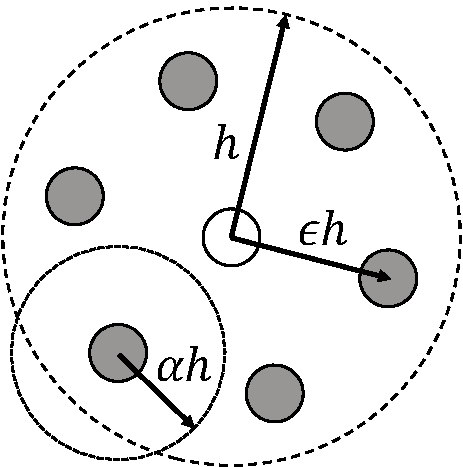
\includegraphics[scale=0.6]{particle_splitting_draw.pdf}
  \centering
  \caption{Particle splitting pattern with the notation of the separation parameter $\epsilon$ and smoothing ratio $\alpha$. Empty circle shows the original particle and the filled ones are the generated daughter particles.}
  \label{fig:splitting}
\end{figure}\vspace*{3pt}
To preserve the linear and angular momenta of the mother particle during the splitting and ensure the exact conservation of mass, the
\begin{equation}
\begin{split}
m_m=n_pm_d, \\
v_m=v_d
\end{split}
\end{equation}
expressions must hold, where $m_m$ and $m_d$ are the mass of the mother and daughter particles, $v$ is the velocity and $n_p$ is the number of the daughter particles. Beside the change of the mass per particle, one also need to change the particle smoothing radius using the $\alpha$ smoothing ratio. Without shifting its center off mass, the daughter particles are placed around the mother particle using the separation parameter $\epsilon$.

\textbf{Particle coalescing}\\
Opposite to the particle splitting, coalescing facilitates the particle number reduction when less detailed solution is required in a specific region. The particle merging procedure implemented in Nauticle ensured the exact conservation of not only the mass and linear momentum, but the angular momentum as well. In contrast with former coalescing procedures, this can be done by merging a particle triplet to a pair of particles having sufficient degrees of freedom to preserve a rotational motion \cite{Toth2018}. The particle merging procedure is shown in Figure \ref{fig:merging}.
\begin{figure}[H]
  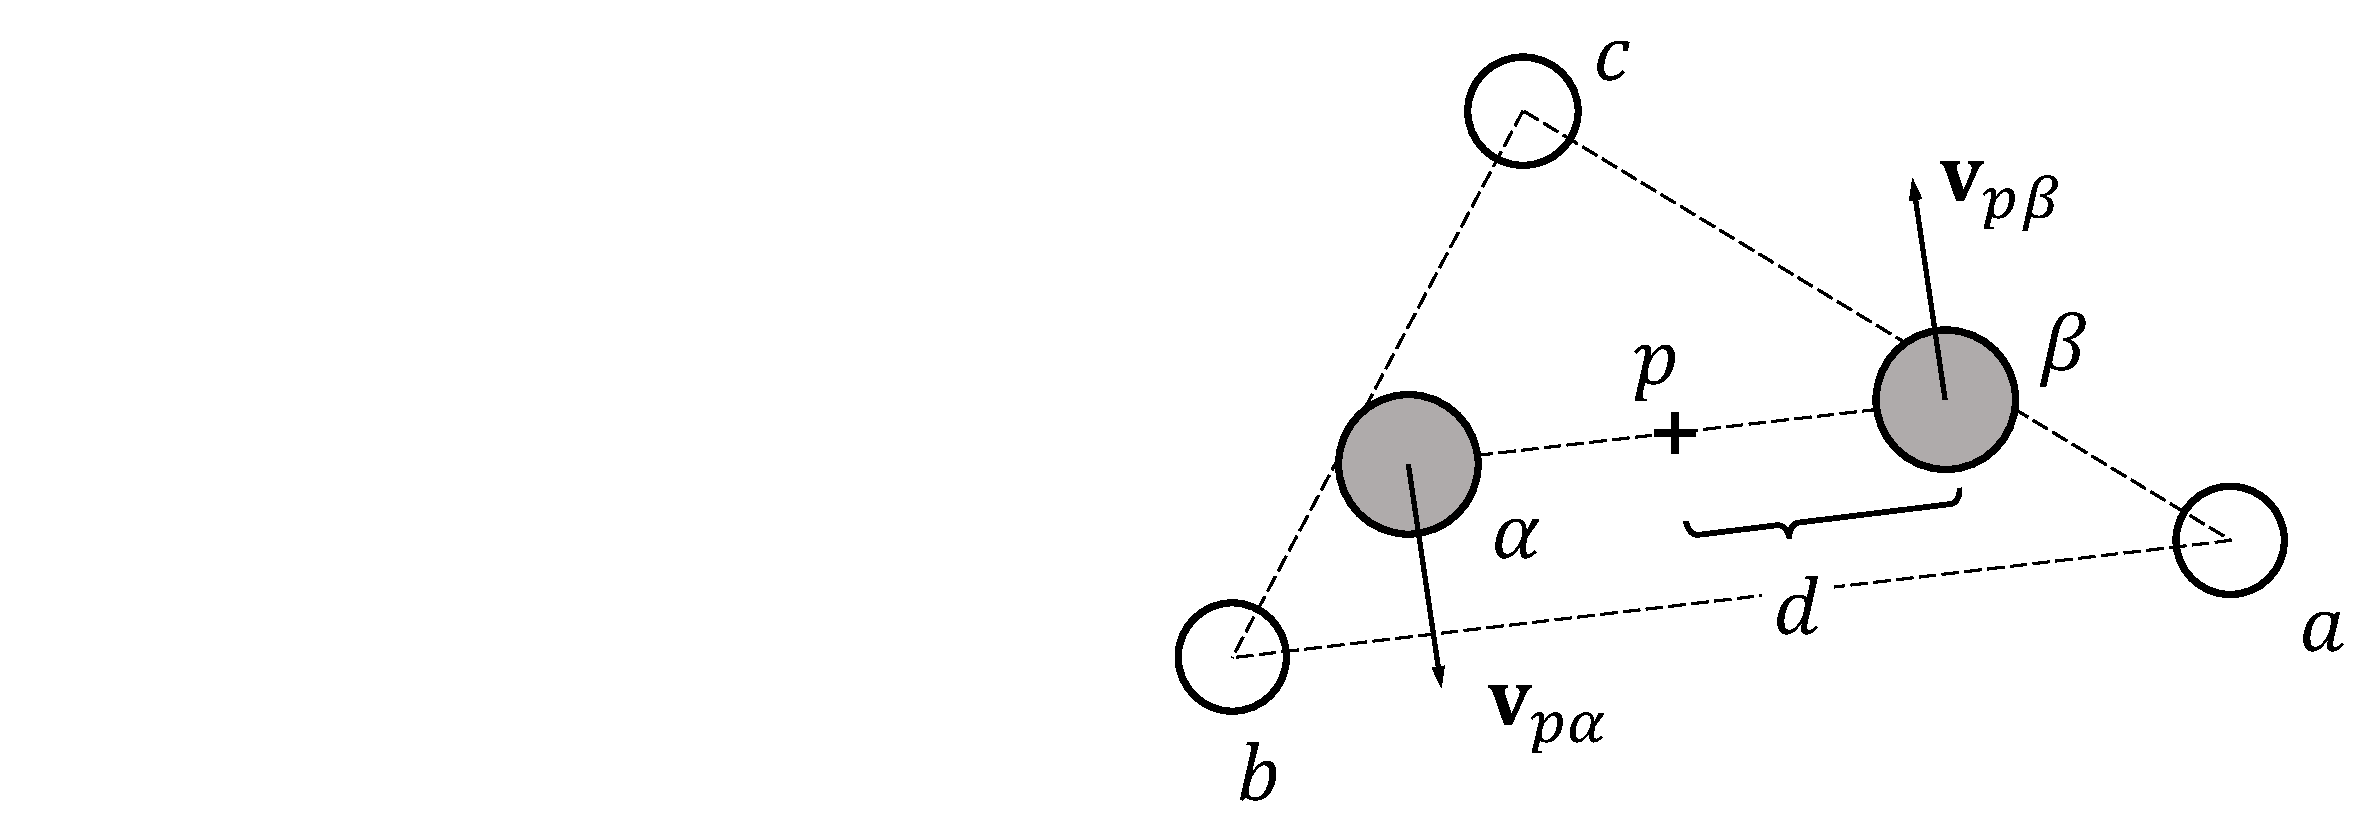
\includegraphics[scale=0.4]{particle_coalescing_draw.pdf}
  \centering
  \caption{Particle coalescing technique with angular momentum conservation. Empty circles show the original particle and the filled ones show the layout after merge.}
  \label{fig:merging}
\end{figure}\vspace*{3pt}


\subsubsection{Discrete Element Method (DEM)} \label{sec:DEM_intro}
In contrast to SPH, Discrete Element Method (DEM) provides a formulation for modeling discontinuous materials through direct calculation of interaction forces between colliding elements. DEM was introduced by P.A. Cundall in 1971 \cite{Cundall1971} for particles with identical, regular shapes. Later the method was extended to particles with irregular shapes by M.A. Taylor et al. in 2006 \cite{Taylor2006}.
% Today, a wide variety of normal and tangential contact force model exists based on different physical assumptions.
The method is suitable to exploit the general potentials of particle methods such as parallelisation and it became one of the most famous particle-based tools for modelling the motion of granular materials in engineering applications. In Nauticle the implemented DEM model assumes rotationally invariant spherical particles with varying radii. 
\myparagraph{Equations of motion}
The motion of particle $i$ in space can be described by Newton's second law
\begin{flalign} \label{eq:restrictionDEM_EOM}
\begin{split}
&m_i\frac{d^2\textbf{r}_i}{dt^2}=\textbf{F}_i+m_i \textbf{g}, \\
&\bm{\Theta}_i\frac{d\bm{\omega}_i}{dt}=\textbf{T}_i,
\end{split}
\end{flalign}
where $\textbf{r}_i$ is the position vector, $m_i$ and $\bm{\Theta}_i$ are the mass and moment of inertia, $\textbf{F}_i$ and $\textbf{T}_i$ are the resultant force and torque corresponding to particle $i$. Due to its high complexity, the deformation of particles is neglected, instead the collision forces are calculated using the overlap length
\begin{flalign} \label{DEM_interactions}
&\delta_{ij}=(R_i+R_j)-\vert\textbf{r}_j-\textbf{r}_i\vert
\end{flalign}
between particle $i$ and $j$, where $R$ is the particles' radii. The layout and notations of the collision of two adjecent particles are shown in Figure \ref{fig:collision}.
\begin{figure}[H]
  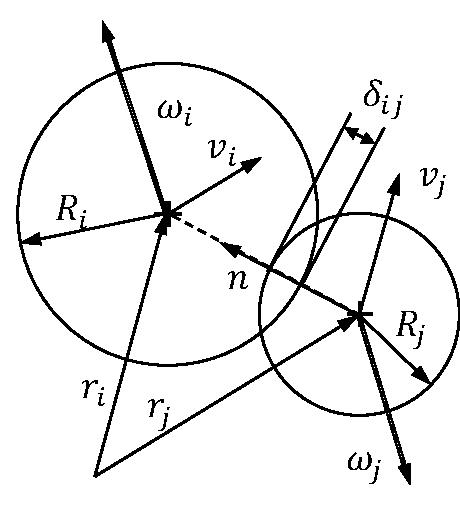
\includegraphics[scale=0.8]{collision.pdf}
  \centering
  \caption{Particle collision layout with the length of overlap $\delta$.}
  \label{fig:collision}
\end{figure}\vspace*{3pt}
The interaction force $F_i$ and torque $T_i$ in \equref{eq:restrictionDEM_EOM} can be determined using the collision model
\begin{flalign} \label{DEM_interactions}
&\textbf{F}_i=\sum_{j}{\left(\textbf{F}^n_{ij}+\textbf{F}^t_{ij}\right)}, \\
&\textbf{T}_i=\sum_{j}{\textbf{T}_{ij}},
\end{flalign} itself
with $F_{ij}^n$ and $F_{ij}^t$ being the normal and tangential forces and $T_{ij}$ is the torque acting from particle $j$ to $i$.
\myparagraph{Normal contact force model}
The abovementioned overlapping length anneals the collision response of rigid objects by the $\delta$-dependent repulsive normal contact force model based on the Hertzian stress and damping
\begin{flalign} \label{DEM_normal_force}
&\textbf{F}_{ij}^n=-(k_{Hz}\delta^{3/2}+c_{Hz}\delta^{1/4})\textbf{n}_{ji},
\end{flalign}
where
\begin{align} \label{DEM_Hertzian_spring}
&k_{Hz} = \frac{4}{3}\sqrt{R'}E', \\
&c_{Hz} = \frac{\sqrt{m'k_{Hz}}}{8}
\end{align}
are the spring and damping coefficients of the collision in normal direction with the effective quantities
\begin{align}
&R'=\frac{R_iR_j}{R_i+R_j}, \\
&m'=\frac{m_im_j}{m_i+m_j}, \\
&E'=\frac{E_iE_j}{E_j(1-\nu_i^2)+E_i(1-\nu_j^2)}.
\end{align}

\myparagraph{Tangential contact force and torque model}
The tangential or shear forces between colliding particles are determined by the relative linear and angular velocities $\textbf{v}_{ij}$ and $\bm{\omega}_{ij}$. The tangential contact force model is written as
\begin{flalign} \label{DEM_tangential_force}
&\textbf{F}_{ij}^t=\phi\vert\textbf{F}_{ij}^n\vert\textbf{t}_{ij},
\end{flalign}
where $\phi $ is the tangential Coulomb-friction coefficient and
\begin{gather}
\textbf{t}_{ij}=\frac{\textbf{v}^t}{\vert\textbf{v}^t\vert} \\
\textbf{v}^t=-\textbf{v}_{ij}+(\textbf{v}_{ij}\textbf{n}_{ji})\textbf{n}_{ji}+\bm{\omega}_i\times\bigg(R_i-\frac{\delta}{2}\bigg)\textbf{n}_{ji} + \bm{\omega}_j\times\bigg(R_j-\frac{\delta}{2}\bigg)\textbf{n}_{ji}.
\end{gather}
The tangential contact forces are used to calculate the resultant torque of particle $i$:
\begin{flalign} \label{DEM_tangential_force}
&\textbf{T}_i=\sum_j{R_i'\textbf{n}_{ji}\times \textbf{F}_{ij}^t}.
\end{flalign}
Note that particle interaction forces and torques are calculated only when $\delta>0$, otherwise, the particles $i$ and $j$ are not in interaction with each other.

The equations \equref{eq:restrictionDEM_EOM} form a system of $N$ algebraic equations that can be solved explicitly.\\


\subsubsection{Discrete Vortex Method (DVM)} \label{sec:DVM}
Vortex methods are meshless numerical tools for modeling inviscid fluid flow governed by point vortices. The basic idea behind vortex methods is that vorticity is a conserved quantity in inviscid flows, consequently, the flow field can be determined using a set of point vortices drifting in the velocity field induced by themselves \cite{DVM_URL}.

First of all the vorticity is defined as the curl of the velocity field $\textbf{v}$:
\begin{flalign} \label{DVM_vorticity}
&\bm{\omega}=\nabla\times \textbf{v}.
\end{flalign}
For incompressible fluids the continuity equation reduces to
\begin{flalign} \label{DVM_continuity}
&\nabla\cdot\dot{\textbf{v}}=0,
\end{flalign}
which can be automatically satisfied by introducing the vector streamfunction $\Psi$ such that
\begin{flalign} \label{DVM_vector_streamfunction}
&\textbf{v}=\nabla\times\Psi.
\end{flalign}
By assuming the vector streamfunction to be divergence free, the vorticity can now be expressed as
\begin{flalign} \label{DVM_vector_poisson}
&\bm{\omega}\nabla\times\nabla\times\Psi=\nabla(\nabla\dot\Psi)-\nabla^2\Psi=-\nabla^2\Psi,
\end{flalign}
the vector Poisson's equation for the streamfunction. Equation \equref{DVM_vector_poisson} in case of a single point vortex at position $\textbf{r}_0$ with vorticity strength $\bm{\omega}$ in infinite domain has the form
\begin{flalign} \label{DVM_poisson_single}
\nabla^2\Psi=-\bm{\omega}\frac{\delta(|\textbf{r}-\textbf{r}_0|)}{2\pi |\textbf{r}-\textbf{r}_0|}.
\end{flalign}
The solution of \equref{DVM_poisson_single} can be obtained by Green's function:
\begin{flalign} \label{DVM_streamfunction_single}
\Psi(\textbf{r})=-\bm{\omega}(\textbf{r}_0)\frac{ln|\textbf{r}-\textbf{r}_0|}{2\pi}.
\end{flalign}
The corresponding velocity field is calculated by
\begin{flalign} \label{DVM_velocity_single}
\textbf{v}(\textbf{r})=\nabla\times\Psi=\frac{\bm{\omega}\times (\textbf{r}-\textbf{r}_0)}{2\pi |\textbf{r}-\textbf{r}_0|^2}.
\end{flalign}
Considering the linearity of \equref{DVM_poisson_single} one can calculate the flow field induced by multiple vortex points by simply summing up the contributions of the individual vortices:
\begin{flalign} \label{DVM_velocity_multi}
\textbf{v}(\textbf{r})=\sum_i\frac{\omega_i\times (\textbf{r}-\textbf{r}_i)}{2\pi |\textbf{r}-\textbf{r}_i|^2}.
\end{flalign}
The implication of point vortices may cause stability problems due to the singular velocity field at the point vortices. To circumvent such condition it is required to use vortex blobs instead of point vortices. A second order Gaussian approximation of the velocity in \equref{DVM_velocity_multi} is written as:
\begin{flalign} \label{DVM_velocity_multi_blob}
\textbf{v}(\textbf{r})=\sum_i\frac{\omega_i\times (\textbf{r}-\textbf{r}_i)}{2\pi |\textbf{r}-\textbf{r}_i|^2}(1-e^{-|\textbf{r}-\textbf{r}_i|^2/\epsilon^2}),
\end{flalign}
where $\epsilon$ is the width of the Gaussian kernel. This approximation eliminates the numerically unmanageable high velocities in the immediate vicinity of vortex points but provides accurate velocity contribution elsewhere. The associated velocity field advects the vortex points in space without changing their strength of vorticity. Obviously the new layout of vortex points induces a different velocity field providing the subsequent instant of the time-dependent inviscid flow. 

Although there are several variants of vortex methods involving boundary conditions as constraints analogously to the Methods of Fundamental Solutions (MFS), only the basic Discrete Vortex Method is implemented in Nauticle.

\subsubsection{Standard Social Force Model (SFM)} \label{sec:SFM}
Evacuation time and efficiency acquire crucial importance during the design process of modern buildings. The demand of safety protocols facilitates the research of crowd motion under predefined conditions. During the recent decades, several models of different fundamentals were built to simulate the flow of people in buildings of complex geometries based on the fundamental work of D. Helbing and P. Molnár \cite{Helbing1995}. More recent models like \cite{Tissera2012} (analogy with fluid mechanics) or \cite{Li2015} (implying Cellular Automata (CA)) were built to simulate large scale dynamics of pedestrians.

The standard Social Force Model is a micro-scale deterministic model considering the intentions of each individual person as driving forces besides the repulsive forces during collisions of their bodies.
One of the simplest driving force is included in the equation
\begin{flalign} \label{SFM_ode}
&\frac{d\textbf{v}_i}{dt}=\frac{v_0\textbf{e}_0-\textbf{v}_i}{\tau}-\frac{1}{m_i}\sum_{j\neq i}{\bigg[A_i exp\bigg(\frac{R_{ij}-d_{ij}}{B_i}\bigg)+k(R_{ij}-d_{ij})-c_{ij}\bigg]\textbf{n}_{ji}},
\end{flalign}
where $v_i$ is the velocity of the $i^{th}$ person, $v_0$ is the desired velocity magnitude in the direction $e_0$ and $\tau$ is the time scale. Furthermore, $A_i$, $B_i$, $k$ are constants of repulsive, $c_{ij}$ is of attractive forces, $R_{ij}=R_i+R_j$ is the sum of the radii of the two individuals in collision. $\textbf{n}_{ji}$, as formerly, is the normalized direction vector pointing from person $i$ to $j$, and finally, $d_{ij}$ is the distance between them. The desired velocity vector $v_0e_0$ is continually changing as the person moves towards the desired position. The equation \equref{SFM_ode} forms the basic social force interactions implemented in Nauticle.

\subsubsection{Molecular dynamics (MD)} \label{sec:MD}
The current Nauticle release implements a minimal molecular dynamics model governed by the Lennard-Jones potential:
\begin{flalign} \label{LJ_potential}
V(r)=4\epsilon\bigg(\bigg(\frac{\sigma}{r}\bigg)^{12}-\frac{1}{2}\bigg(\frac{\sigma}{r}\bigg)^6\bigg),
\end{flalign}
which can be used to calculate the interaction forces between particles $i$ and $j$:
\begin{flalign} \label{LJ_interaction}
\textbf{f}_{ji}=\frac{dV}{dr}\bigg|_{\vert\textbf{r}_{ji}\vert}=\frac{48\epsilon}{\vert\textbf{r}_{ji}\vert^2}\bigg(\bigg(\frac{\sigma}{\vert\textbf{r}_{ji}\vert}\bigg)^{12}-\frac{1}{2}\bigg(\frac{\sigma}{\vert\textbf{r}_{ji}\vert}\bigg)^6\bigg)\textbf{r}_{ji},
\end{flalign}
where $\textbf{r}_{ji}=\textbf{r}_{j}-\textbf{r}_{i}$. The constant parameters $\epsilon$ and $\sigma$ define the interaction magnitude and particle radii respectively. Although the potential function is unbounded, it is beneficial to apply an $r_{cut}=3\sigma$ to avoid $\O(N^2)$ complexity without significant loss of accuracy. The potential \equref{LJ_potential} implies two interparticle effects, namely the long range attraction, and a short range and strong repulsion forces. These are represented by the $(\sigma/r)^6$ and $(\sigma/r)^{12}$ terms respectively.

The equation of motion of the molecular system according to \equref{LJ_interaction} reads as:
\begin{flalign} \label{LJ_ode}
\ddot{\textbf{r}}_{i}=-\sum_{j\neq i}{\textbf{f}_{ji}}.
\end{flalign}



\subsubsection{Kuramoto model} \label{sec:kuramoto}
The model implemented in Nauticle can be considered as a generalization of the conventional Kuramoto model \cite{Kuramoto1975}. Conventionally, the synchronization of phase oscillators can be expressed as the solution of the equation
\begin{equation} \label{eq:kuramoto}
\dot\theta_i=\Omega_i+\frac{K}{N}\sum_{j=1}^N{\sin(\theta_j-\theta_i)} \quad\quad\quad i=1,..,N,
\end{equation}
where $\theta_i$ is the phase of the $i$th oscillator, $\Omega$ is the natural frequency, $K$ is the coupling strength, $N$ is thw number of coupled oscillators in the system. Although the equation \equref{eq:kuramoto} has several different form, even with higher order temporal derivatives \cite{Tanaka1997}, in the present discussion we focus on the second term on the right hand side. Implying spatial connectivity, several works investigate diluted systems with a binary connectivity matrix $A_{ij}$ such that $A_{ij}=1$ if the oscillators $i$ and $j$ are connected and $A_{ij}=0$ if not \cite{Olmi2014}. The synchronization term then reads as
\begin{equation}
\frac{K}{N}\sum_{j=1}^N{A_{ij}\sin(\theta_j-\theta_i)}.
\end{equation}
As another approach implemented in Nuticle, the oscillator connectivity can be considered using the spatial configuration:
\begin{equation}
\begin{split}
&K\sum_{j=1}^N{\sin(\theta_j-\theta_i)\hat W_{ij}}, \\
&\hat W_{ij}=\frac{W_{ij}}{\sum_j{W_{ij}}}
\end{split}
\end{equation}
where $W_{ij}$ is a smoothing kernel function.


\subsection{Temporal integration}
Numerical schemes for integration are required to solve time-dependent differential equations. Two numerical schemes are implemented in Nauticle.
\subsubsection{Explicit-Euler method}
This is a one-step explicit method to advance quantities in time by the
\begin{flalign}
\phi^{n+1}=\phi^n+\Delta t f(\phi^n,t^n)
\end{flalign}
expression, where $\phi$ is an arbitrary quantity, $f(\phi^n,t^n)$ is a function of $\phi$ and time $t$ in the $n$th time instant, and $\Delta t=t^{n+1}-t^n$ is the time step size.
\subsubsection{Second-order Runge-Kutta method}
The second order explicit Runge-Kutta or midpoint scheme consists of two integration steps. The first one is the prediction step
\begin{flalign}
\phi^{n+1/2}=\phi^n+\frac{\Delta t}{2} f(\phi^n,t^n),
\end{flalign}
which is followed by the evaluation of $f(\phi^{n+1/2},t^{n+1/2})$. The second step is the correction step to obtain the final value $\phi^{n+1}$:
\begin{flalign}
\phi^{n+1}=\phi^n+\Delta t f(\phi^{n+1/2},t^{n+1/2}).
\end{flalign}
\subsubsection{Velocity-Verlet method}
A common choice for integration of second order equation of motion is the velocity-Verlet method. The algorithm reads as:
\begin{flalign}
&x^{n+1}=x^n+v^n\Delta t+\frac{a^n}{2}\Delta t^2, \\
&v^{n+1}=v^n+\frac{a^n+a^{n+1}}{2}\Delta t.
\end{flalign}
As can be seen, it is assumed that the acceleration $a^{n+1}$ does not depend on $v^{n+1}$.

\section{Implementation}
\subsection{The Nauticle environment} \label{sec:environment}
The basic idea of the Nauticle environment is that any particle method (regardless of the classification in Section \ref{sec:particle_method_classification}) can be considered as the determination of interactions between spatially distributed point-like nodes (particles). This assumption leads to the general interpretation of particle methods as \textit{interactions} (read more about the interactions in Section \ref{sec:interface}). 

In this section the definitions corresponding to Nauticle are introduced, then the most important implementation methodologies and features of the solver are discussed.
\subsubsection{Definitions} \label{sec:definitions}
\textbf{Tensor}: Tensors in Nauticle have a few restrictions that are discussed here for the sake of clarity and simplicity. The tensor $\textbf{T}$ is a zeroth ($\textbf{T}\in\R$), first ($\textbf{T}\in\R^d$), or second ($\textbf{T}\in\R^d\otimes\R^d$) order real valued tensor, in $d=1,2,3$ dimensions. Throughout this guide tensors are considered to obey these restrictions, otherwise, it is indicated. Furthermore, all the quantities (scalar, vector, and tensor) are represented by tensors.

\textbf{Domain}: Consider the simply connected rectangular subset $\Gamma^d\subset\R^d$ ($d=1,2,3$), with edge size $\bm{\lambda}\in\R$ and its boundary $\partial\Gamma^d$. The $\Gamma^d$ subset is a $d$ dimensional domain, if the
\begin{flalign}
\begin{split}
&1.\quad \Gamma^d=[\textbf{r}_{min},\textbf{r}_{max}] \puretext{such that} \textbf{r}_{min}<\textbf{r}_{max} \puretext{and} \{\textbf{r}_{min},\textbf{r}_{max}\} \in \R^d\\
&2.\quad \partial\Gamma^d=\bigcup_{d}{(\textbf{r}_{min}\cup \textbf{r}_{max})} \\
&3.\quad \bm{\lambda}=\textbf{r}_{max}-\textbf{r}_{min}
\end{split}
\end{flalign}
conditions are satisfied.

\textbf{Particle}: A point-like object with position $\textbf{r}\in\Gamma^d$.

\textbf{Particle system}: The $\textbf{P}_{N}=\left\{\textbf{r}_i|i=1,2,...,N\right\}$ set of particles $\textbf{r}_i\in\Gamma^d$ is defined as a particle system of domain $\Gamma^d$.

\textbf{Field}: Consider a particle system $\textbf{P}_N$ of particles $\textbf{r}_i$, $i=1,2..N$. The set $\textbf{F}_N=\left\{\textbf{f}_i\leftarrow \textbf{r}_i \vert i=1,2,...,N\right\}$ is a field over $\textbf{P}_N$ if $\textbf{f}_i$ is a real valued zeroth, first or second order tensor associated to particle $i$.

\subsection{n-nearest neighbor search} \label{sec:neighbor_search}
One of the specific properties of particle methods is the continually changing particle layout. Since no interparticle structure is considered, the connectivity may change (except for Lagrangian or unbounded mollifier functions) with the particle positions. The naive ($N^2$ complexity) determination of particle interactions is usually unsatisfactory due to its high-performance requirement, therefore a more efficient neighbor searching algorithm should be used instead \cite{CUDA_EXAMPLE}. Here a simple and memory-efficient algorithm is implemented. The basic idea of the method is that a so-called hash key is assigned to each particle depending on the cell it occupies. Since all the particles that occupy the same cell obtain identical hash keys, the list of particles of the adjacent cells can be constructed easily.

The bottleneck of this algorithm is that the particle positions need to be sorted by the hash keys, which can be computationally expensive. However, when the particle layout does not change too much before the recalculation of the hash keys, the sorting process is cheap because most of the particle's hash keys are already organized in the proper order.\\
\begin{figure}[H]
  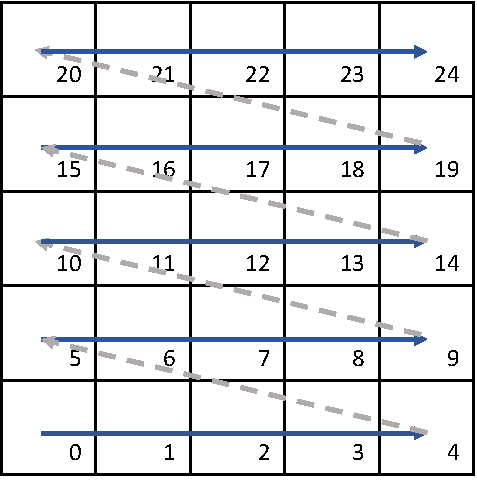
\includegraphics[scale=0.6]{hash_key.pdf}
  \centering
  \caption{Unfolding the two-dimensional domain to one dimension. The same procedure can be applied in three dimensions.}
  \label{fig:unfolding}
\end{figure}\vspace*{3pt}
\begin{figure}[H]
  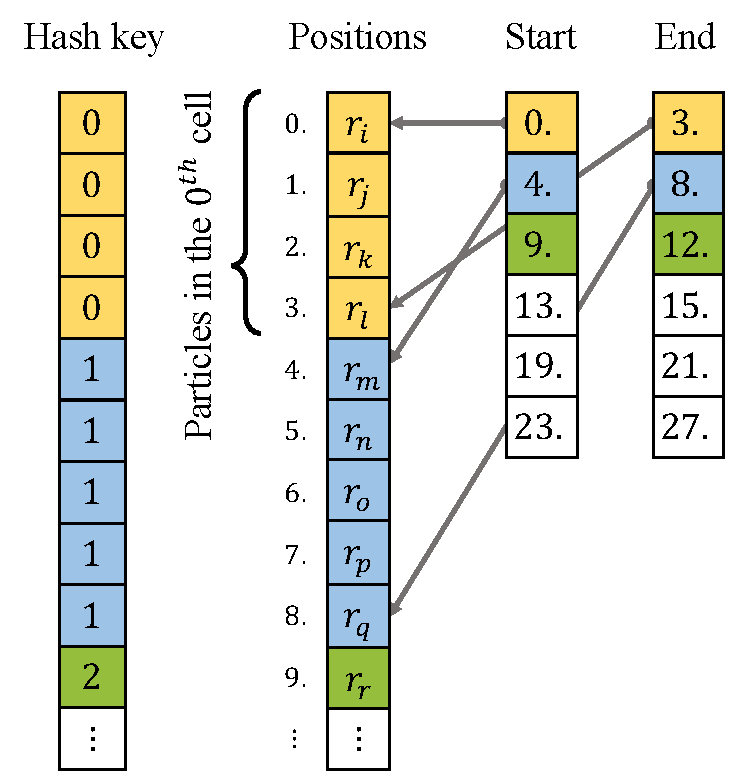
\includegraphics[scale=0.6]{nnsearch.pdf}
  \centering
  \caption{Indexing particle positions with Start and End arrays.}
  \label{fig:nnsearch}
\end{figure}\vspace*{3pt}

To determine interparticle connectivity the following steps are performed in Nauticle:
\begin{enumerate}
  \item Calculation of a hash key for each particle using the unfolding of the domain shown by Figure \ref{fig:unfolding},
  \item Sorting particles and the fields by the array of hash keys,
  \item Generating Start and End arrays containing the index of the first and last particle of each cell. The Start and End arrays are introduced in Figure \ref{fig:nnsearch}.
\end{enumerate}
Later, during the calculation of particle interactions, the particles of the adjacent cells of each particle are checked using the start and end arrays to mark the potential neighbors. Finally, the actual neighbors are calculated based on the set of potential neighbors.
Particle neighbor search is automatically managed during any simulation in Nauticle.

\subsection{Periodic, symmetric and cut-off boundaries} \label{sec:boundaries}
The computational domain $\Omega$ defined in Section \ref{sec:definitions} forms the particles' frame of reference. Since no particle can ever exist outside the domain, the bounding surface $\partial\Omega$ applies symmetric or periodic rules to avoid the exclusion by handling particles that intend to cross the surface. One more special case, a cut-off boundary is implemented as well to avoid undesirable interactions. Obviously, the opposite boundaries of $\Omega$ have to be both periodic, symmetric or cut-off boundaries.
Each type of boundary conditions imply the repositioning of exiting particle $i$ applying the
\begin{flalign} \label{eq:restriction}
\textbf{r}_i\leftarrow \textbf{r}_i mod \lambda
\end{flalign}
restriction, where $\lambda$ is the size of $\Omega$. However, exiting should ideally never occur in case of a symmetric boundary. The restriction \equref{eq:restriction} does not provide either correct periodic or symmetric boundary conditions in itself. To take these conditions into account, the overhanging influence radius should be replaced or reflected properly. The physical interpretation of influence radius in the vicinity of periodic ($\partial\Omega_p$) and symmetric ($\partial\Omega_s$) boundaries is shown in Figure \ref{fig:periodic_symmetric}.
\begin{figure}[H]
  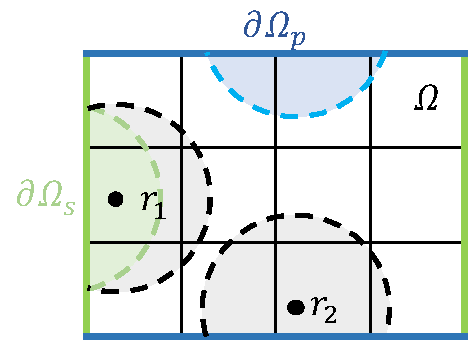
\includegraphics[scale=0.8]{periodic_symmetric_2.pdf}
  \centering
  \caption{ Shifting (blue) and reflecting (green) influence radius in the vicinity of periodic and symmetric boundary conditions respectively.}
  \label{fig:periodic_symmetric}
\end{figure}\vspace*{3pt}
During the calculation of interparticle distance vector $\textbf{r}_{ji}=\textbf{r}_j-\textbf{r}_i$ at the boundary the ensemble formula
\begin{flalign} \label{eq:boundary_interparticle_distance}
&\textbf{r}^\alpha_{ji}\leftarrow \textbf{r}^\alpha_{ji}+\bm{\beta}^\alpha\bm{\delta}^\alpha(\bm{\delta}^\alpha-1)(\textbf{r}^\alpha_{max}-\textbf{r}^\alpha_j)+\bm{\beta}^\alpha\bm{\delta}^\alpha(\bm{\delta}^\alpha+1)(\textbf{r}^\alpha_{min}-\textbf{r}^\alpha_j)+(\bm{\beta}^\alpha-1)\bm{\delta}^\alpha\bm{\lambda}^\alpha
\end{flalign}
is applied in each axis aligned directions $\alpha=x,y,z$, where $\beta=0$ or $1$ for periodic or symmetric boundaries respectively, $\lambda$ is the size of $\Omega$, the operator $\floor{\cdot}$ denotes floor, $\bm{\delta}$ is given by
\begin{flalign} \label{eq:delta_perioic_symmetric}
&\bm{\delta}=-\floor{\frac{\textbf{g}_j-\textbf{r}_{min}}{N_c}},
\end{flalign}
with $\textbf{g}_j$ being the grid coordinate of particle $j$ and $N_c$ denotes the number of cells along the edges of $\Omega$. The grid coordinates of the adjacent particles is calculated by
\begin{flalign} \label{eq:grid_position_periodic_symmetric}
&\textbf{g}_j\leftarrow \textbf{g}_j+\bm{\delta}(N_c-\bm{\beta} N_c+\bm{\beta}).
\end{flalign}
Since in case of the symmetric condition the interactions are calculated by particle mirroring, the vector and tensor quantities should be reflected using the reflection matrix
\begin{flalign} \label{eq:reflection_periodic_symmetric}
&\textbf{R}=\textbf{I}^d(-2\bm{\beta}_i+1),
\end{flalign}
where $I^d$ is a $d$ dimensional identity tensor.

Note that in case of certain quantities like angular velocity, or vorticity the reflection \equref{eq:reflection_periodic_symmetric} could be physically incorrect. Such cases are required to be treated with attention at symmetric boundaries by marking a field as non-symmetric (see the details in Section \ref{sec:DVM_example}).


\subsection{Symbolic form language (SFL) - Class hierarchy of expressions}
The generality of the numerical solver requires the analysis of user-defined expressions and equations. In Nauticle the expression parsing is based on the class hierarchy of expressions shown in Figure \ref{fig:expression_tree}.
\begin{figure}[H]
  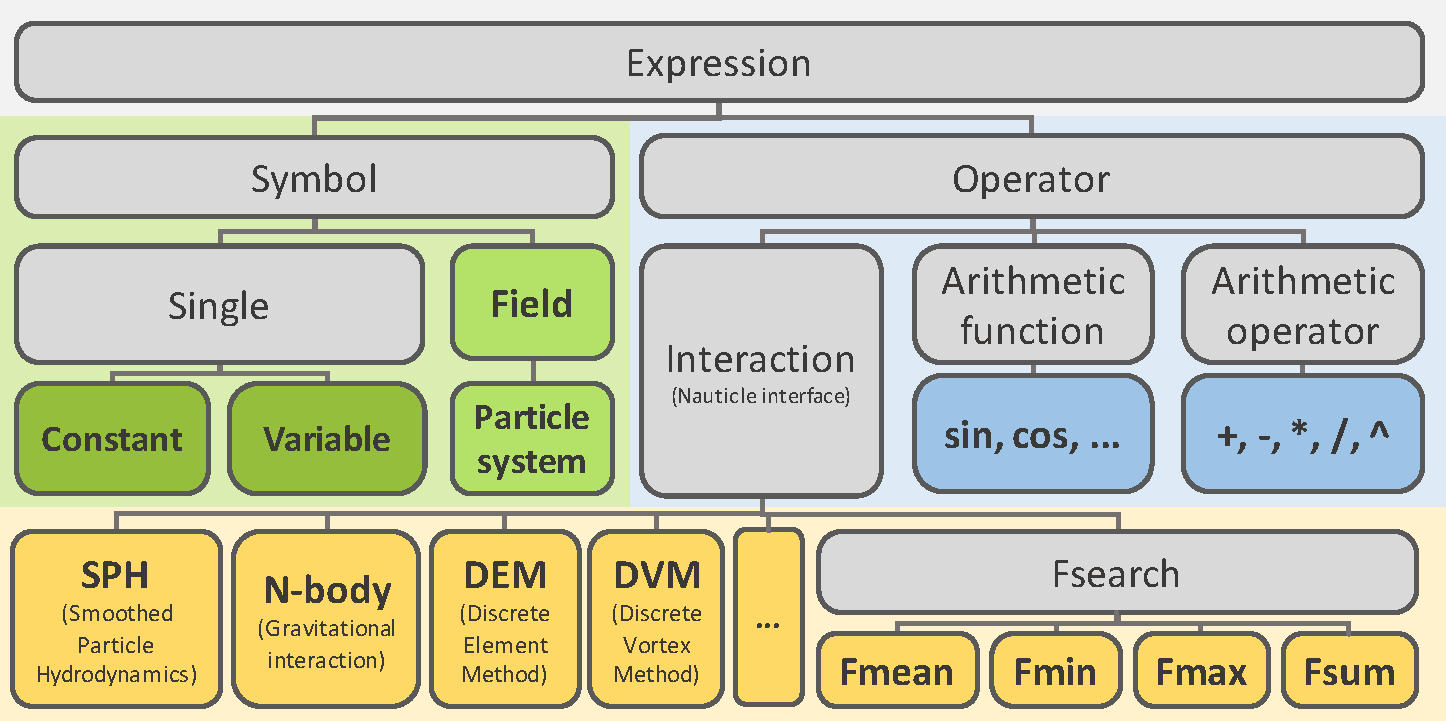
\includegraphics[scale=0.5]{expression_tree.pdf}
  \centering
  \caption{Expression tree: hierarchy of expression elements. The gray nodes in the tree indicate abstract types.}
  \label{fig:expression_tree}
\end{figure}\vspace*{3pt}

After the transformation of a user-defined expression to Reverse Polish Notation (RPN), the nodes of the expression tree can be employed to interpret the expression and perform its solution recursively. A simple example is presented by Figure \ref{fig:expression_example}.
\begin{figure}[H]
  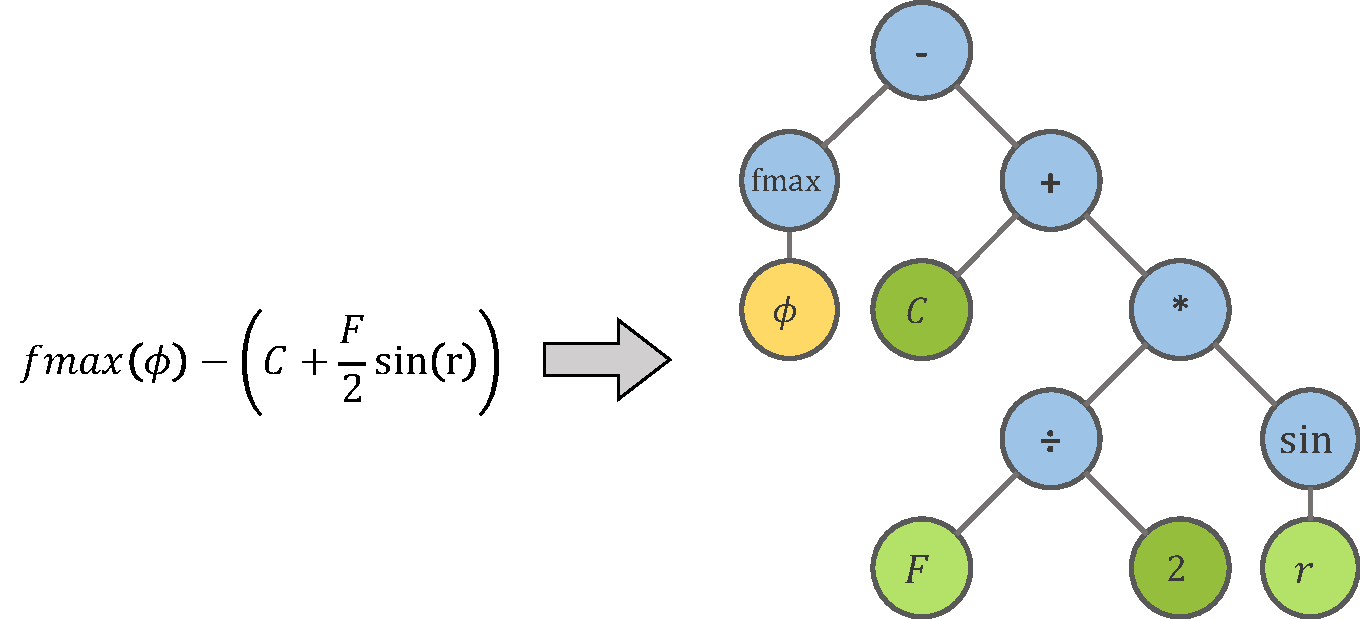
\includegraphics[scale=0.5]{expression_example.pdf}
  \centering
  \caption{Example for construction of expressions using the nodes of the expression tree.}
  \label{fig:expression_example}
\end{figure}\vspace*{3pt}

Although the nodes of the hierarchy specify different quantities and operators of Nauticle, all nodes are considered to operate on tensors. In the following, the branches and nodes of the expression tree are discussed.

\subsubsection{The symbol branch}
On the one hand, the single symbols like constants and variables represent global values for the simulation (such as the time step size or gravitational acceleration), which usually have the same value for each particle, consequently, one (single) instance is sufficient to be stored. Therefore the single quantities have very small memory requirements. However, in case of multistep integrators, the desired number of previous values of variables are automatically stored. Obviously it is unnecessary for constant values since they cannot be changed during their lifetime. On the other hand, the fields are interpreted over a set of spatial nodes (particles) storing tensor values assigned to each of the particles. Former values for multistep integrators are automatically stored as well, as in case of the variables. A special implementation of a field is the particle system itself, storing the particle positions as field variables. The particle system is special not only because it stores particle positions but it performs n-nearest neighbor search and stores the computational domain too. The restriction \equref{eq:restriction} of particles to the domain is also performed by the particle system.

\subsubsection{The operator branch}
The other main branch of the hierarchy is the branch of operators acting on symbols. Operators are classified into three groups:
\begin{itemize}
  \item Arithmetic operators,
  \item Arithmetic functions,
  \item Interactions.
\end{itemize}
The first two groups of operators evaluate operations on single quantities or particlewise field quantities (e.g. addition of two fields), while the interactions require field data (e.g. value of field maximum or minimum).
\myparagraph{Arithmetic operators}
The supported arithmetic operators are presented in Table \ref{tbl:arop}.
\begin{table} [hbt!]
\begin{center}
\caption{Supported arithmetic operators in Nauticle.}\label{tbl:arop}
\begin{tabular}{ l c c c c }
\toprule[1.5pt]
\bf Operator name & \bf Sign & \bf Operands & \bf Description\\ 
\midrule
Addition & "+" & 2 & $[n \times m] + [n \times m]$\\ 
Subtraction & "-" & 2 & $[n \times m] - [n \times m]$\\ 
Product & "*" & 2 & $[n \times m] * [m \times n]$\\ 
Division & "/" & 2 & $[n \times m] / [1 \times 1]$\\ 
Term by term product & ":" & 2 & $[n \times m] : [n \times m]$\\ 
Term by term division & "\%" & 2 & $[n \times m] \% [n \times m]$\\ 
Power & "$\hat{\ }$" & 2 & $[n \times m] \hat{\ } [1 \times 1]$\\ 
Positive & "+" & 1 & $+[n \times m]$\\ 
Negative & "-" & 1 & $-[n \times m]$\\ 
\bottomrule[1.25pt]
\end{tabular}
\end{center}
\end{table}
The arithmetic operators are valid for tensors with conforming sizes (last column of Table \ref{tbl:arop}).
\myparagraph{Arithmetic functions} \label{sec:functions}
The arithmetic functions supported by Nauticle are summarized in Table \ref{tbl:arfc}. It should be noted here that complex numbers are currently not supported by the tensor implementation, therefore some of the functions may give indefinite results (e.g. $\sqrt{-1}$ is not a number in Nauticle).
\begin{table} [H]
\begin{center}
\caption{Supported arithmetic functions in Nauticle.}\label{tbl:arfc}
\begin{tabular}{ l l c | l l c }
\toprule[1.5pt]
\bf Funcion & \bf Name & \bf Op's & \bf Funcion & \bf Name & \bf Op's\\ 
\midrule
Absolute value & $abs$ & 1 & Modulo & $mod$ & 2 \\
Arc cosine & $acos$ & 1 & Random in range & $rand$ & 2 \\
Arc co-tangent & $acot$ & 1 & Sign & $sgn$ & 1 \\
Arc sine & $asin$ & 1 & Sine & $sin$ & 1 \\
Arc tangent & $atan$ & 1 & Sine hyperbolic & $sinh$ & 1 \\
Cosine & $cos$ & 1 & Square root & $sqrt$ & 1 \\
Cosine hyperbolic & $cosh$ & 1 & Tangent & $tan$ & 1 \\
Co-tangent & $cot$ & 1 & Tangent hyperbolic & $tanh$ & 1 \\
Co-tangent hyperbolic & $coth$ & 1 & Trace & $trace$ & 1 \\
Cross product & $cross$ & 2 & Transpose & $transpose$ & 1 \\
Exponential & $exp$ & 1 & Truncation & $trunc$ & 1 \\
Floor & $floor$ & 1 & Matrix determinant & $determinant$ & 1 \\
Greater than & $gt$ & 2 & Matrix inverse & $inverse$ & 1 \\
Greater than or equal & $gte$ & 2 & Logical condition & $if$ & 3 \\
Less than & $lt$ & 2 & Equal & $eq$ & 2 \\
Less than or equal & $lte$ & 2 & Not equal & $neq$ & 2 \\
Natural logarithm & $log$ & 1 & Logical and & $and$ & 2 \\
Vector length & $magnitude$ & 1 & Logical or & $or$ & 2 \\
Maximum & $max$ & 2 & Logical negation & $not$ & 1 \\
Minimum & $min$ & 2 & Logical exclusive or & $xor$ & 2 \\
Tensor element & $elem$ & 3 & Identity tensor & $identity$ & 1 \\
Q tensor of QR dec. & $deQ$ & 1 & R tensor of QR dec. & $deR$ & 1 \\ 
Matrix eigenvectors & $eigsys$ & 1 & Matrix eigenvalues & $eigval$ & 1 \\
Matrix logarithm & $logm$ & 1 & Limit & $limit$ & 3 \\
\bottomrule[1.25pt]
\end{tabular}
\end{center}
\end{table}

Since numerical integrators form a special group of the arithmetic functions, they are summarized separately in Table \ref{tbl:arfc_int}. 
\begin{table} [H]
\begin{center}
\caption{Supported arithmetic functions in Nauticle.}\label{tbl:arfc_int}
\begin{tabular}{ l l c }
\toprule[1.5pt]
\bf Funcion & \bf Name & \bf Operands \\ 
\midrule
Explicit Euler & $euler$ & \multirow{3}{*}{$A$, $\dot A$, $\Delta t$}   \\
RK2 predictor & $predictor$ & \\
RK2 corrector & $corrector$ &  \\
Verlet position & $verlet\_r$ & $r$, $\dot r$, $\ddot r$, $\Delta t$ \\
Verlet velocity & $verlet\_v$ & $\dot r$, $\ddot r$, $\Delta t$ \\
\bottomrule[1.25pt]
\end{tabular}
\end{center}
\end{table}

\myparagraph{Interactions} \label{sec:interactions}
It was pointed out earlier in Section \ref{sec:environment} that any particle method can be considered as a collection of particle interaction laws. Accordingly, the interaction branch forms an essential part of not only the expression tree but also the Nauticle environment. This group of operators deals with particle interactions that certainly depend on field quantities (and the particle system). Furthermore, the interaction branch provides an intermediate development interface, which is introduced in detail later in Section \ref{sec:interface}.
The simplest functions in this branch are presented in Table \ref{tbl:fsearch}. Since the magnitude of an arbitrary tensor quantity is ambiguous, these field-functions can be evaluated only over scalar fields (last column of Table \ref{tbl:fsearch}). These functions have approximately linear computational complexity.
\begin{table}[H]
\begin{center}
\caption{Simple interaction operators.}\label{tbl:fsearch}
\begin{tabular}{ l l c c }
\toprule[1.5pt]
\bf Operator & \bf Name & \bf Operands & \bf Description\\
\midrule
Field maximum & $fmax$ & 1 & $[1 \times 1]$\\ 
Field minimum & $fmin$ & 1 & $[1 \times 1]$\\ 
Field average & $fmean$ & 1 & $[n \times m]$\\
Field sum & $fsum$ & 1 & $[n \times m]$\\
\bottomrule[1.25pt]
\end{tabular}
\end{center}
\end{table}

Further interaction operators in Nauticle summarized below are related to the operators of the particle methods presented in Section \ref{sec:implemented} providing the opportunity of simultaneous application of any of the interaction operators. For a deeper explanation of the implementation of interaction operators refer to Section \ref{sec:interface}.

First of all, it is beneficial to understand the built-in filter functions, which form the basis of some of the particle methods. The implemented filter functions (kernels) in Nauticle are enumerated below.

\textbf{Zeroth order}:
\begin{flalign} \label{eq:kernel_zeroth_order}
W^{zeroth}(q)=\alpha_D,
\end{flalign}
where $D$ is the number of the dimensions, $\alpha_1=0.5/\sigma$, $\alpha_2=2/(\pi \sigma^2)$ and $\alpha_3=3/(4\pi \sigma^3)$ are the normalization coefficients, and $q=|r|/\sigma$ with the smoothing distance $\sigma$. The influence radius of the zeroth order kernel equals $q$.

\textbf{First order}:
\begin{flalign} \label{eq:kernel_first_order}
W^{first}(q)=\alpha_D(1-q),
\end{flalign}
where, $\alpha_1=1/\sigma$, $\alpha_2=3/(\pi \sigma^2)$ and $\alpha_3=3/(\pi \sigma^3)$. The influence radius of the first order kernel equals $q$.

\textbf{Second order polynomial (quadratic)}:
\begin{flalign} \label{eq:kernel_quadratic}
W^{quadratic}(q)=\alpha_D\bigg(\frac{3}{16}q^2-\frac{3}{4}q+\frac{3}{4}\bigg)
\end{flalign}
Here $\alpha_1=1/\sigma$, $\alpha_2=2/(\pi \sigma^2)$ and $\alpha_3=5/(4\pi \sigma^3)$ and $q=|r|/\sigma$ with the smoothing distance $\sigma$. The influence radius of the quadratic kernel equals $2q$. 

\textbf{Third order polynomial (cubic)}:
% \[
\begin{equation}
    W^{cubic}(q)= \alpha_D
\begin{cases}
  1-\frac{3}{2}q^2+\frac{3}{4}q^3;  & \text{if } q\leq1\\
  \frac{1}{4}(2-q)^3& \text{if } 1 < q \leq 2
\end{cases}
\end{equation}
% \]
Here $\alpha_1=2/(3\sigma)$, $\alpha_2=10/(7\pi \sigma^2)$ and $\alpha_3=1/(\pi \sigma^3)$. The influence radius of the cubic kernel also equals $2q$.

\textbf{Fifth order polynomial (quintic)}:
\begin{flalign} \label{eq:kernel_quintic}
W^{quintic}(q)=\alpha_D\bigg(1-\frac{q}{2}\bigg)^4(2q+1)
\end{flalign}
Here $\alpha_1=3/(4h)$, $\alpha_2=7/(4\pi \sigma^2)$ and $\alpha_3=21/(16\pi \sigma^3)$. And again, the influence radius of the quintic kernel equals $2q$.

\textbf{Gaussian}:
\begin{flalign} \label{eq:kernel_quintic}
W^{Gaussian}(q)=\alpha_D\exp\bigg(-\frac{q^2}{4}\bigg)
\end{flalign}
The normalisation coefficients are $\alpha_1=1/(\sigma\sqrt{2\pi})$, $\alpha_2=1/(2\pi \sigma^2)$ and $\alpha_3=1/(2\pi \sigma^2)^{3/2}$. The influence radius of the Gaussian kernel is infinite.

Meshless interpolants often do not require the kernel function itself but its derivative, therefore the first order derivative of the presented kernels are also included. To apply any of the filter kernels in Nauticle, a simple identifier explained in Figure \ref{fig:kernel_explanation} is associated with them.
\begin{figure}[H]
  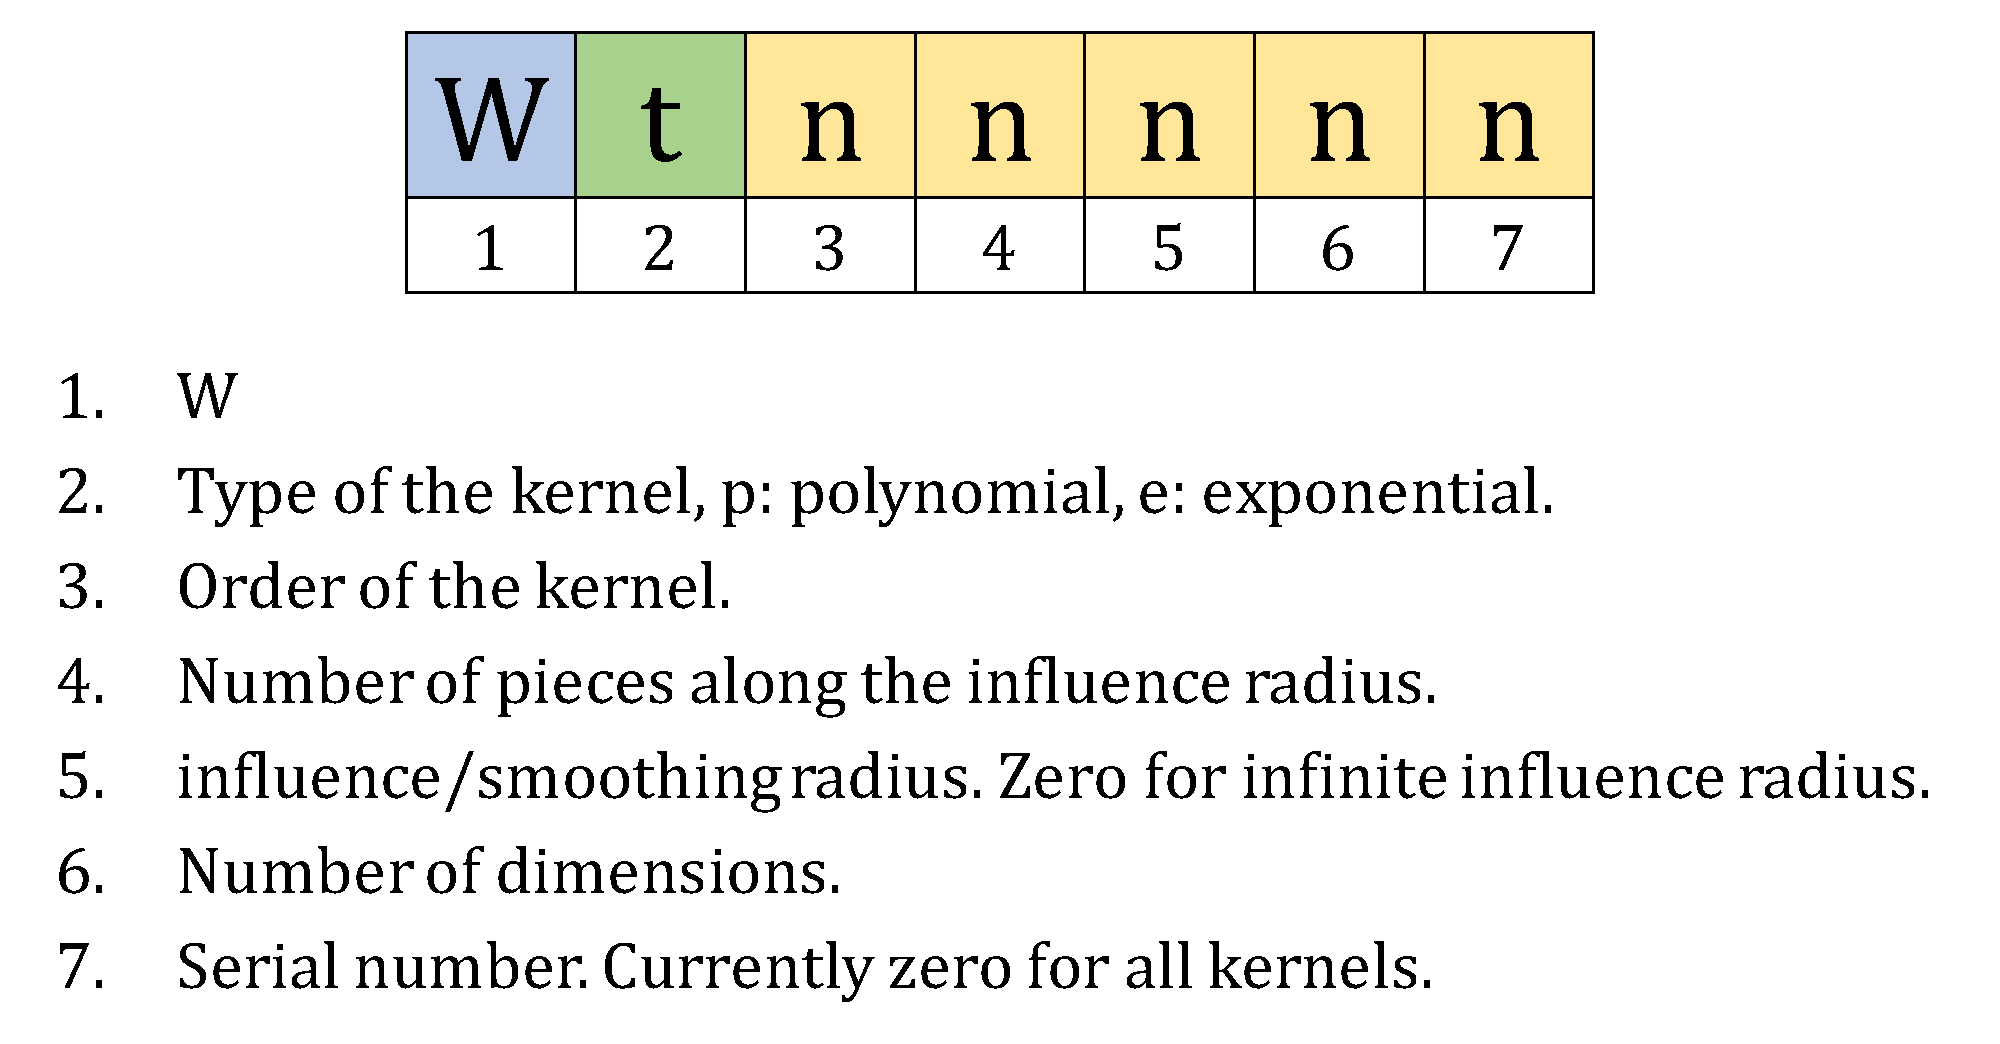
\includegraphics[scale=0.3]{kernel_explanation.pdf}
  \centering
  \caption{Explanation of the identifier associated to filter kernels.}
  \label{fig:kernel_explanation}
\end{figure}

\mysubparagraph{N-body operator}
The simplest implemented scheme in Nauticle, namely the gravitational N-body problem is simply considered as a single interaction operator identical to the RHS of \equref{eq:nbody_eom}, described in Table \ref{tbl:nbody_op}.
\begin{table} [hbt!]
\begin{center}
\caption{N-body problem operator.}\label{tbl:nbody_op}
\begin{tabular}{ l c l }
\toprule[1.5pt]
\bf Name & \bf Operands & \bf Description \\ 
\midrule
$nbody$ & $m$, $\gamma$ & $\frac{d^2\textbf{r}_i}{dt^2}=\gamma\sum_j^N{\frac{m_im_j}{(\textbf{r}_j-\textbf{r}_i)^2}\textbf{n}_{ji}}$ \\ 
\bottomrule[1.25pt]
\end{tabular}
\end{center}
\end{table}
Obviously, mass $m$ is allowed to be a particlewise varying field, while gravitational constant $\gamma$ is a true single value, even if a field is provided. In the latter case the zeroth value of the field is used over each interaction. The $nbody$ operator has quadratic computational complexity due to the infinite gravitational influence radius. Note that it is not recommended to use this operator on particles close to the domain boundary of any type, furthermore, neither periodic nor symmetric boundary conditions are suitable to simulate infinite patterns of self-gravitating particle cloud.

\mysubparagraph{SPH operators}
In this section the usage of the same operators as in Section \ref{sec:SPH_intro} are discussed without the deduction of the interpolants.
\begin{table} [h!]
\begin{center}
\caption{SPH operators.}\label{tbl:sph_op}
\begin{tabular}{ l c l }
\toprule[1.5pt]
\bf Name & \bf Operands & \bf Description \\ 
\midrule
$sph\_S$ & \multirow{21}{*}{$A$, $m$, $\rho$, $W$, $R_{infl}$} & $\langle A_i\rangle=\sum_j{A_jW_{ij}\frac{m_j}{\rho_j}}$ \\ [2ex]
$sph\_X$ &  & $\langle\hat{A}_i\rangle=\sum_j{(A_j-A_i)W_{ij}\frac{m_j}{\rho_j}}$ \\ [2ex]
$sph\_G$ &  & $\langle grad(A_i)\rangle=\sum_j{A_j\otimes\nabla W_{ij}\frac{m_j}{\rho_j}}$ \\ [2ex]
$sph\_G00$ &  & $\langle grad(A_i)\rangle=\sum_j{(A_j-A_i)\otimes\nabla W_{ij}\frac{m_j}{\rho_j}}$ \\ [2ex]
$sph\_G01$ &  & $\langle grad(A_i)\rangle=\frac{1}{\rho_i}\sum_j{(A_j-A_i)\otimes\nabla W_{ij}m_j}$ \\ [2ex]
$sph\_G10$ &  & $\langle grad(A_i)\rangle=\sum_j{(A_j+A_i)\otimes\nabla W_{ij}\frac{m_j}{\rho_j}}$ \\ [2ex]
$sph\_G11$ &  & $\langle grad(A_i)\rangle=\rho_i\sum_j{\big(\frac{A_j}{\rho_j^2}+\frac{A_i}{\rho_i^2}\big)\otimes\nabla W_{ij}m_j}$ \\ [2ex]
$sph\_D$ &  & $\langle div(A_i)\rangle=\sum_j{A_j\nabla W_{ij}\frac{m_j}{\rho_j}}$ \\ [2ex]
$sph\_D00$ &  & $\langle div(A_i)\rangle=\sum_j{(A_j-A_i)\nabla W_{ij}\frac{m_j}{\rho_j}}$ \\ [2ex]
$sph\_D01$ &  & $\langle div(A_i)\rangle=\frac{1}{\rho_i}\sum_j{(A_j-A_i)\nabla W_{ij}m_j}$ \\ [2ex]
$sph\_D10$ &  & $\langle div(A_i)\rangle=\sum_j{(A_j+A_i)\nabla W_{ij}\frac{m_j}{\rho_j}}$ \\ [2ex]
$sph\_D11$ &  & $\langle div(A_i)\rangle=\rho_i\sum_j{\big(\frac{A_j}{\rho_j^2}+\frac{A_i}{\rho_i^2}\big)\nabla W_{ij}m_j}$ \\ [2ex]
$sph\_L0$ &  & $\langle\Delta A_i\rangle=\sum_{j}{2(A(\textbf{r}_i)-A(\textbf{r}_j))\frac{\textbf{r}_j-\textbf{r}_i}{\vert \textbf{r}_j-\textbf{r}_i \vert^2}\nabla W_{ij}\frac{m_j}{\rho_j}}$ \\ [2ex]
$sph\_L1$ & $B$, $A$, $m$, $\rho$, $W$, $R_{infl}$ & $\langle \nabla (B_i \nabla A_i)\rangle=\sum_{j}{2(B_j-B_i)(A_j-A_i)\frac{\textbf{r}_j-\textbf{r}_i}{\vert \textbf{r}_j-\textbf{r}_i \vert^2}\nabla W_{ij}\frac{m_j}{\rho_j}}$ \\ [2ex]
$sph\_I$ & $r$, $m$, $\rho$, $W$, $R_{infl}$ & $\langle I(\textbf{r}_i)\rangle=\sum_{j}{(\textbf{r}_j-\textbf{r}_i)(\textbf{r}_j-\textbf{r}_i)W(\textbf{r}_i-\textbf{r}_j,\sigma)\frac{m_j}{\rho_j}}$ \\ [2ex]
$sph\_A$ & $v$, $m$, $\rho$, $W$, $R_{infl}$ &$\frac{d\textbf{v}^{av}_i}{dt}=\sum_{j}{\Pi_{ij}m_j\nabla W(\textbf{r}_i-\textbf{r}_j,\sigma)}$ \\ [2ex]
$sph\_T$ & $dx$ $p$, $m$, $\rho$, $W$, $R_{infl}$ &$\frac{d\textbf{v}^{ap}_i}{dt}=-\sum_{j}{\textbf{R}_{ij}f^n\nabla W(\textbf{r}_i-\textbf{r}_j,\sigma)m_j}$ \\ [2ex]
\bottomrule[1.25pt]
\end{tabular}
\end{center}
\end{table}
The gradient, divergence and Laplacian operators are denoted by $G$, $D$ and $L$ respectively, $R_{infl}$ is the influence radius and $\otimes$ refers to the outer product. Although divergence and gradient operators are distinguished by the product type, they give the same result in certain cases, for instance in one dimension or if $A$ is scalar.

\mysubparagraph{DEM operators}
As it is shown in Section \ref{sec:DEM_intro} the particle motion is governed by two separate ordinary differential equations, consequently the linear and angular motion have to be treated separately. The two individual DEM operators are described in Table \ref{tbl:DEM_ops} including the same notations as in Section \ref{sec:DEM_intro}.
\begin{table} [h!]
\begin{center}
\caption{Operators of the Discrete Element Method.} \label{tbl:DEM_ops}
\begin{tabular}{ l c l }
\toprule[1.5pt]
\bf Name & \bf Operands & \bf Description \\ 
\midrule
$dem\_l$ & \multirow{2}{*}{$v, \omega, R, m, E, \nu, \phi$} & $\textbf{F}_i=\sum_{j}{\left(\textbf{F}^n_{ij}+\textbf{F}^t_{ij}\right)}$ \\ 
$dem\_a$ &  & $\textbf{T}_i=\sum_{j}{\textbf{T}_{ij}}$ \\ 
\bottomrule[1.25pt]
\end{tabular}
\end{center}
\end{table}
Except for the Coulomb-friction coefficient $\phi$, all the operands of both linear and angular operators are allowed to be field quantities.


\mysubparagraph{DVM operator}
The implementation of the DVM scheme is covered by a single operator introduced in Table \ref{tbl:DVM_op}. 
\begin{table} [h!]
\begin{center}
\caption{Operator of the Discrete Vortex Method.} \label{tbl:DVM_op}
\begin{tabular}{ l c l }
\toprule[1.5pt]
\bf Name & \bf Operands & \bf Description \\ 
\midrule
$dvm$ & $\omega, \epsilon$ & $\textbf{v}(\textbf{r})=\sum_i\frac{\bm{\omega}_i\times (\textbf{r}-\textbf{r}_i)}{2\pi \vert\textbf{r}-\textbf{r}_i\vert^2}(1-e^{-\vert\textbf{r}-\textbf{r}_i\vert^2/\epsilon^2})$ \\
\bottomrule[1.25pt]
\end{tabular}
\end{center}
\end{table}
Although in theory the interactions of the DVM operator have infinite influence radii, the implementation suffers from a cutoff distance error caused by the finite cell sizes of the domain. However in such a case, both periodic and symmetric boundary conditions can be employed properly.



\mysubparagraph{SFM operator}
Similarly to the N-body and DVM operators, the SFM implementation is also covered by a single operator shown by Table \ref{tbl:SFM_op}.
\begin{table} [h!]
\begin{center}
\caption{Operator of the Social Force Model.} \label{tbl:SFM_op}
\begin{tabular}{ l c l }
\toprule[1.5pt]
\bf Name & \bf Operands & \bf Description \\ 
\midrule
$sfm$ & $v,p_0,v_0,m,R,A,B,k,c,\tau$ & $\frac{d\textbf{v}_i}{dt}=$ \\
\bottomrule[1.25pt]
\end{tabular}
\end{center}
\end{table}
The term $f_{ij}$ in the description represents the interaction forces between persons $i$ and $j$ as it was discussed in Section \ref{sec:SFM}. All operands are considered to be fields except for the body-force coefficient $k$ and time-scale $\tau$.

\mysubparagraph{MD operator}
The Lennard-Jones interaction operator is presented in Table \ref{tbl:MD_op}.
\begin{table} [h!]
\begin{center}
\caption{Operator of the Lennard-Jones interaction.} \label{tbl:MD_op}
\begin{tabular}{ l c l }
\toprule[1.5pt]
\bf Name & \bf Operands & \bf Description \\ 
\midrule
$md$ & $\epsilon, \sigma, r_{cut}$ & $\frac{d\textbf{v}_i}{dt}=\sum_{i\neq j}{\textbf{f}_{ji}}$ \\
\bottomrule[1.25pt]
\end{tabular}
\end{center}
\end{table}
The term $f_{ji}$ in the description represents the interaction forces between particles $i$ and $j$ as it was discussed in Section \ref{sec:MD}. All operands are considered to be single and scalar values.

\mysubparagraph{Kuramoto operator}
The Kuramoto interaction operator is presented in Table \ref{tbl:kuramoto_op}.
\begin{table} [h!]
\begin{center}
\caption{Operator of the spatially coupled Kuramoto interaction.} \label{tbl:kuramoto_op}
\begin{tabular}{ l c l }
\toprule[1.5pt]
\bf Name & \bf Operands & \bf Description \\ 
\midrule
$kuramoto$ & $\theta, R, W$ & $\sum_{i\neq j}{\sin(\theta_j-\theta_i)}$ \\
\bottomrule[1.25pt]
\end{tabular}
\end{center}
\end{table}
Here $\theta_i$ is the phase of the $i$th oscillator, R is the influence radius (identical in case of all oscillators) and $W$ is the smoothing kernel function.


\section{Using Nauticle} \label{sec:usage_of_nauticle}
Nauticle is designed not only to simulate a wide range of physical models through user-defined equations but also to form a user- and developer-friendly interface for implementation of arbitrary meshless numerical schemes. As a result, a flexible simulation tool is emerged to facilitate the application of particle-based methods. In Figure \ref{fig:three_levels} the three separated levels of the Nauticle solver is presented and described shortly by pointing out the main aspects of each.
\begin{figure}[H]
  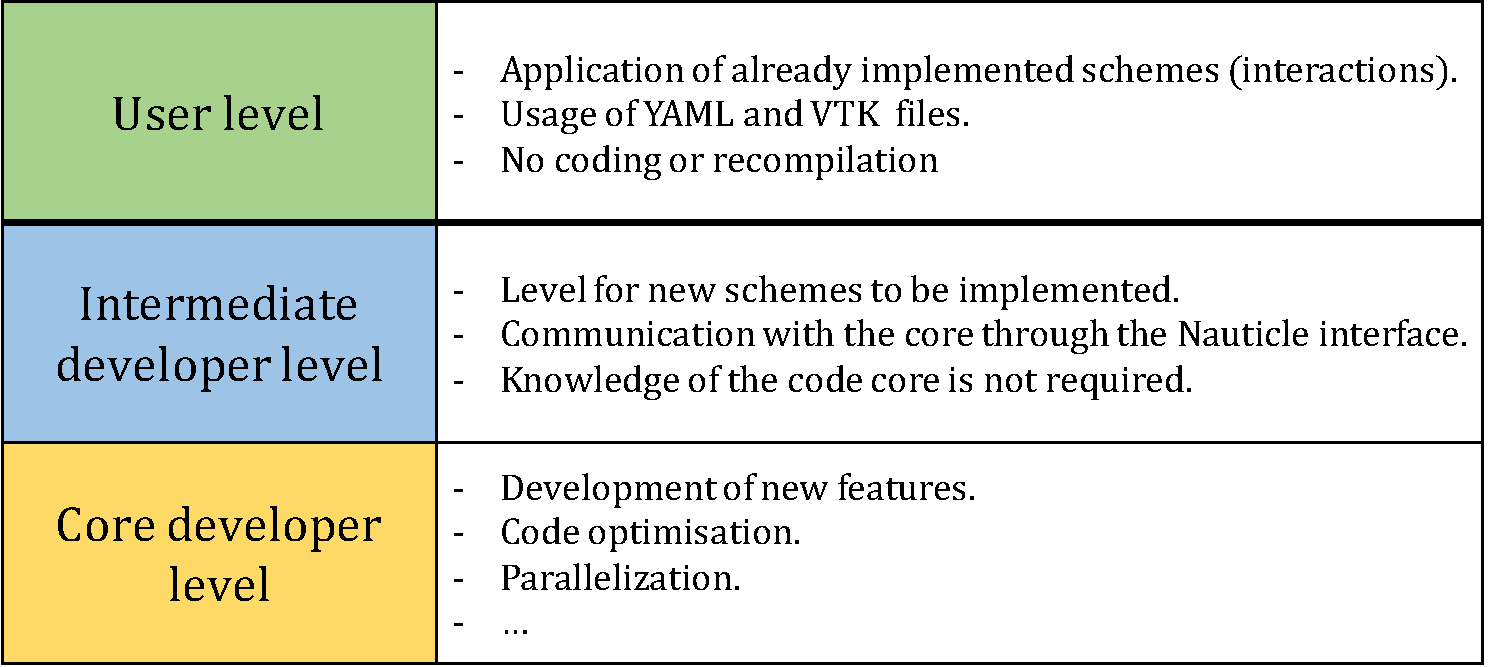
\includegraphics[scale=0.55]{three_levels.pdf}
  \centering
  \caption{Multilevel user and development hierarchy of Nauticle.}
  \label{fig:three_levels}
\end{figure}
This section focuses on the pure user level, where no programming knowledge but the application of YAML forms is required. The core level is out of the scope of this guide, nevertheless, the second, intermediate user and developer level is introduced in section \ref{sec:interface}. 
\subsection{Simulation workflow} \label{sec:sim_workflow}
To define and simulate a problem, a \textit{form} (YAML-document) is needed to be passed to the solver. The form contains all the required information about the physical model called \textit{case}. In this section, the structure of the form is discussed through the introduction of the workspace and the user-defined equations.
\subsubsection{Definitions}
\textbf{Symbol}: User defined constant, variable or field that has a name and a tensor value. Particle system is considered to be a symbol as well.

\textbf{Workspace}: A collection of user-defined symbols representing the quantities of the physical model. The workspace has to contain a particle system with a simulation domain. Field values are assigned to the particle, whereas constants and variables are single values.

\textbf{User-defined equation}: Equation, built up using the nodes of the expression tree and the objects stored in the workspace. The evaluation of an equation means the assignment of the RHS solution to the LHS. Consequently the LHS should be a variable, field or particle system. Each user defined equation has a condition with a default value "true" that determines if the equation has to be solved or not. The condition may have particle-dependent value.

\textbf{Parameter space}: An object to hold information about the simulation and solution data export. The values of the parameters can be expressions that are evaluated in every simulation loop (cf. phase separation model in section \ref{sec:cahn_hilliard}).

\textbf{Splitter / Merger}: Features that allow the user to run computations with spatially varying resolution through particle splitting and merging. Both splitting and merging are governed by different parameters that are evaluated periodically at runtime. Users need to provide fields to the particle modifiers such as mass, velocity and smoothing radius. The complete list and explanation of parameters for the splitter option:
\begin{itemize}
  \item condition: an expression that is evaluated for all particles. If the result is true for a specific particle, it will be splitted in the current simulation loop.
  \item radius\_field: smoothing radius (has to be a field).
  \item rotation: angle of the generated pattern in radians. It is also an expression allowing particle to have different angles, and even randomly distributed angles in space and time.
  \item mass\_field: particle mass (has to be a field).
  \item smoothing\_ratio: the ratio of the new radii and the original particle's radius (expression is allowed).
  \item separation\_parameter: separation parameter of the generated pattern (expression is allowed).
  \item daughters: number of generated particles (expression is allowed).
  \item parent: splitter generates new particle in the place of the original if =1 and not if =0.
  \item period: splitting evaluation frequency (expression is allowed).
\end{itemize}
and for the merger option:
\begin{itemize}
  \item condition: an expression that is evaluated for all particles. If the result is true for a specific particle, it will be merged with its two closest neighbors.
  \item radius\_field: smoothing radius (has to be a field).
  \item mass\_field: particle mass (has to be a field).
  \item velocity\_field: particle velocity (has to be a field).
  \item period: splitting evaluation frequency (expression is allowed).
  \item neighbor\_condition: expression that is evaluated for the neighbors and includes them for merging only if =true.
\end{itemize}
Multiple instances of both splitter and merger options are allowed to be used in a single simulation. Please note, that the currently implemented particle splitting and merging algorithms are working in case of two-dimensional simulations only. A simulation with particle splitting and merging is presented in section \ref{sec:SPH_adaptive}.

\textbf{Background}: external vtkUnstructuredGrid formatted data for particle value (field) interpolation. It requires the file name and the field name that is used to interpolate the grid data periodically in every simulation loop.

\subsubsection{Simulation process}
\begin{figure}[H]
  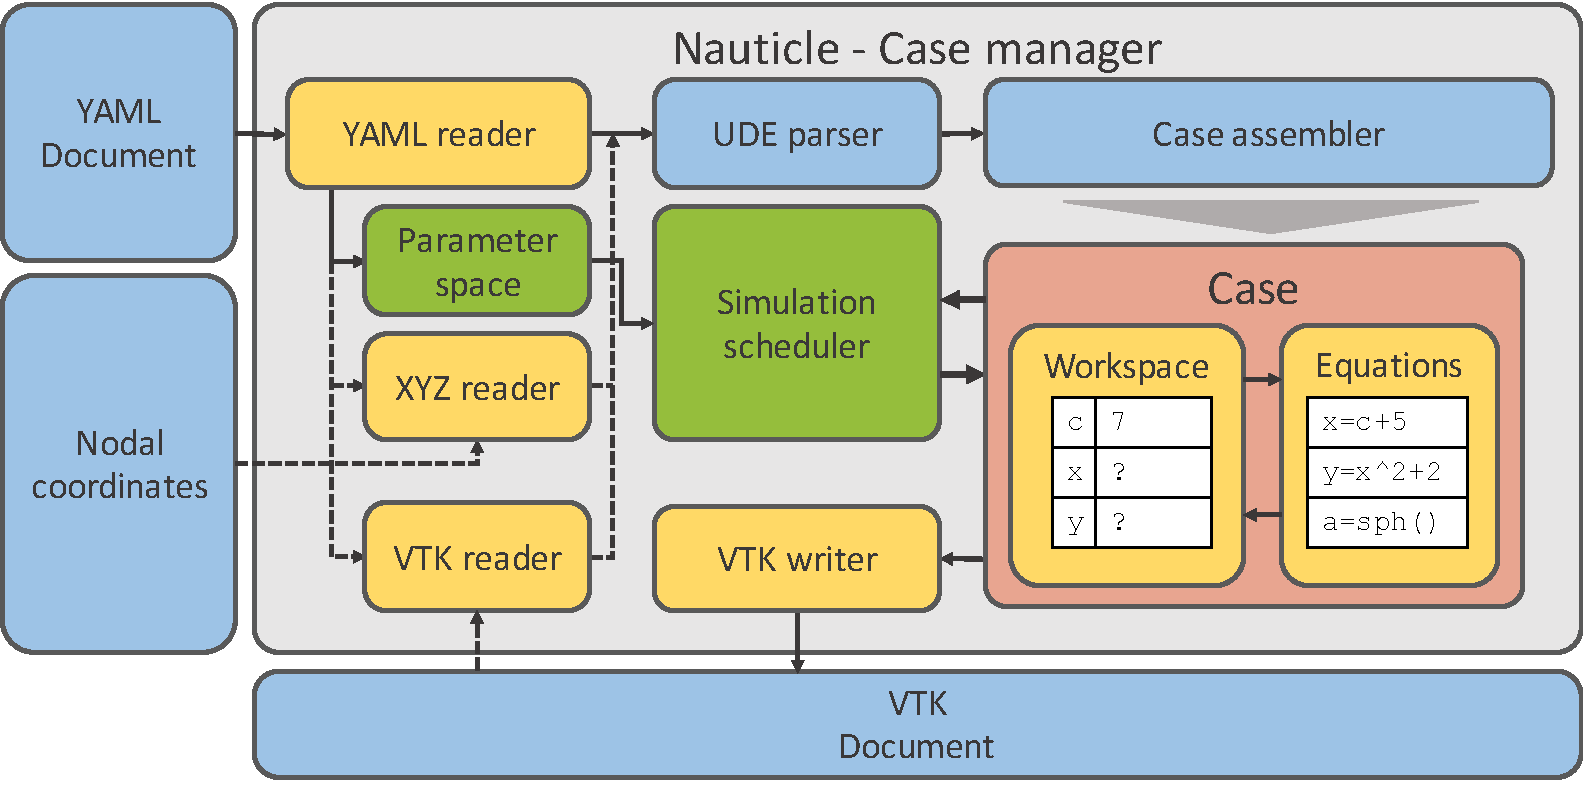
\includegraphics[scale=0.55]{workflow.pdf}
  \centering
  \caption{Outline of the simulation flow.}
  \label{fig:workflow}
\end{figure}

The schematic diagram of a simulation is presented in Figure \ref{fig:workflow}. After the parsing of the input files on the left, the case assembler builds the case, which is handled by the simulation scheduler. The latter is responsible for the calculation flow and parallelization. The result files are saved by the VTK-writer governed by the case manager. 
As soon as the simulation scheduler sends a step request, the solution of the user defined equations is carried out by the case itself. The change of the value of any symbol contained by the workspace during the solution is automatically updated. Optionally, any of the result files can be applied as initial conditions for a further simulation (see Section \ref{sec:YAML}).

\subsection{Runtime compilation of SFL}
From version 1.1.190131 Nauticle supports the automated runtime compilation of user-defined equations constructed in the SFL configuration. To set the runtime compilation active, the \texttt{compile\_case} keyword has to be used in the parameter space:
\begin{example}{Activation of runtime compilation os user-defined equations}{}
\lstset{basicstyle=\tiny}
\begin{lstlisting}[language=YAML]
  parameter_space: 
    simulated_time: 100
    print_interval: 1
    confirm_on_exit: false
    output_format: BINARY
    compile_case: true
\end{lstlisting}
\end{example}
Using this option the runtime compilation is completely automatic without the requirement of any further user actions. With setting the \texttt{compile\_case: true} option, after reading the configuration file, Nauticle performs the following steps:
\begin{itemize}
  \item Makes new folder in the working directory with name \texttt{binary\_case},
  \item Generates \texttt{pmBinary\_case.h} and \texttt{pmBinary\_case.cpp} C++ files in the folder \texttt{binary\_case}. These files hold the whole simulation case defined in the yaml configuration with the workspace and equations,
  \item Generates \texttt{CMakeLists.txt} file with the required header and static library targets including the generated header and source files.
  \item Runs \texttt{CMakeLists.txt} to generate \texttt{Makefile}.
  \item Runs \texttt{Makefile}, to generate the final shared object file \texttt{pmBindary\_case.so},
  \item Loads the shared object and links the binary content to the running application.
  \item Runs the simulation as usual but this time using the compiled objects and functions.
  \item After finishing the computation, Nauticle automatically removes the generated folder.
\end{itemize}

\subsection{Input/Output file formats}
During the execution of a simulation, Nauticle works with four types of input and output files. Some of these files are fundamental, the others are optional. The subsequent sections introduce these file types more or less in the order of importance.
\subsubsection{YAML-document} \label{sec:YAML}
The YAML-document is the most important and fundamental input file of any simulation executed by Nauticle. No simulation can be executed in absence of the configuration YAML-file. Nevertheless, they can be distinguished by the data they contain. The most important advantage of the application of YAML-files is that they support random access to the stored data, therefore the user is not required to follow strict rules during the construction of the simulation problem.\\
\begin{figure}[H]
  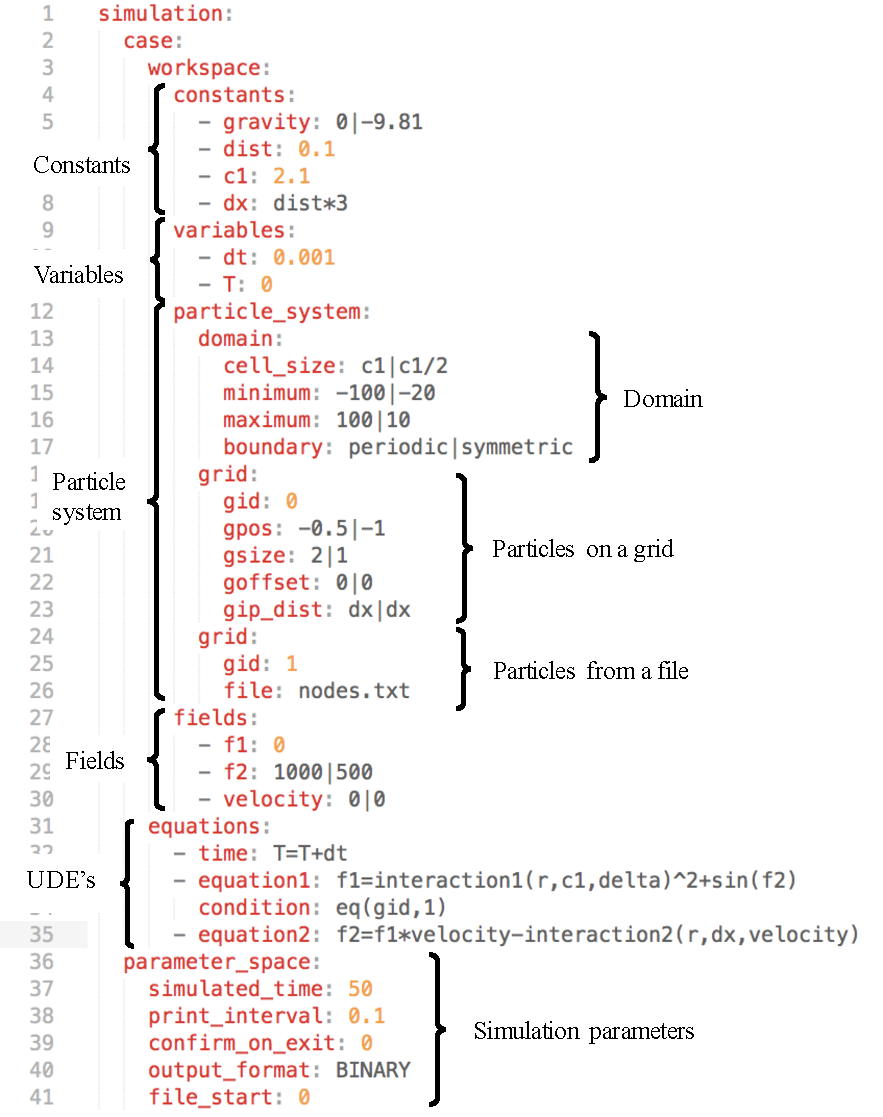
\includegraphics[scale=0.8]{yaml_intro.pdf}
  \centering
  \caption{Structure of the YAML-document.}
  \label{fig:yaml_intro}
\end{figure}\vspace*{3pt}
A simple document is presented in Figure \ref{fig:yaml_intro}, in which the whole workspace and the list of equations to be passed to the solver are defined and no external sources are used except for the nodal coordinates (which is optional). Note that the domain boundaries are defined by the number of cells being integral along each axis. Another way of problem initialization is the application of a former simulation result stored in VTK file. Despite that, YAML-documents cannot be omitted, but are used to refer to the desired input file. This type of initialization allows a significantly simpler YAML-document as it is illustrated in Figure \ref{fig:yaml_intro_simple}.
\begin{figure}[H]
  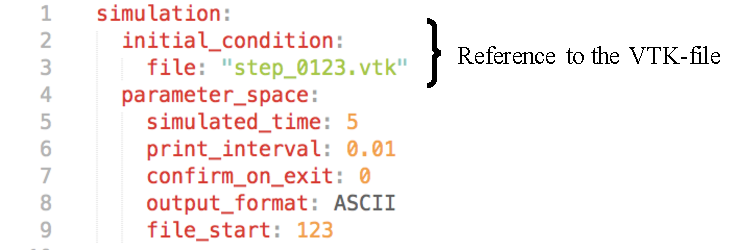
\includegraphics[scale=1]{yaml_intro_simple.pdf}
  \centering
  \caption{Structure of the YAML-document referring to a former simulation result.}
  \label{fig:yaml_intro_simple}
\end{figure}\vspace*{3pt}
\newpage
Note that in this configuration the workspace and list of equations are also stored in the VTK file:\\
\begin{lstlisting}
# vtk DataFile Version 4.0
vtk output
ASCII
DATASET POLYDATA
FIELD FieldData 4
domain 1 4 string
domain_min:-10|-10
domain_max:10|10
cell_size:0.1
boundary:0|1
variables 1 2 string
dt:0.002
T:0
constants 1 3 string
C1:-1.1
C2:3.14159
C3:730
equations 1 3 string
eq1:T=(T+dt)#1
eq2:F1=(C1+F2)#eq(gid,0)
eq3:dt=(C3-C2)#gt(F1,C3)
...
\end{lstlisting}
The character "\#" marks the solution condition for each equation.
\subsubsection{VTK-document}
VTK is a general purpose library for visualization and storage of arbitrary geometry. To store simulation results, VTK formatted ASCII or binary files are used.
\myparagraph{Simple Legacy Formats}
The legacy VTK file formats consist of five basic parts \cite{VTK_format}.
\begin{itemize}
\item 1. The first part is the file version and identifier. This part contains the single line: \# vtk DataFile Version x.x. This line must be exactly as shown with the exception of the version number x.x, which will vary with different releases of VTK. (Note: Nauticle supports version 4.0) 
\item 2. The second part is the header. The header consists of a character string terminated by end-of-line character. The header is 256 characters maximum. The header can be used to describe the data and includes any other pertinent information. 
\item 3. The next part is the file format. The file format describes the type of file, either ASCII or binary. On this line the single word ASCII or BINARY must appear. 
\item 4. The fourth part is the dataset structure. The geometry part describes the geometry and topology of the dataset. This part begins with a line containing the keyword DATASET followed by a keyword describing the type of dataset. Then, depending upon the type of dataset, other keyword/ data combinations define the actual data.
\item 5. The final part describes the dataset attributes. This part begins with the keywords POINT\_DATA or CELL\_DATA, followed by an integer number specifying the number of points or cells, respectively. (It doesn't matter whether POINT\_DATA or CELL\_DATA comes first.) Other keyword/ data combinations then define the actual dataset attribute values (i.e. scalars, vectors, tensors, normals, texture coordinates, or field data). 
\end{itemize}
In Nauticle the result files contain the whole case including the workspace and equations. The DATASET type is POLYDATA, while the symbols and equations are stored as string formatted data.
\subsubsection{Text document}
The particle cloud can be optionally defined through text files containing the set of nodal positions instead of the uniform grid generation based on the YAML data. Note that the text file should always contain three-dimensional coordinates separated by spaces or tabs. The dimensions of the problem are then defined by the domain and only the relevant coordinates of the nodal positions are considered, other coordinates are dropped.
\subsubsection{Log files}
The simulation log file contains the simulation data as it appears in terminal during runtime. Each execution produces a single log file with the name "sim.log" by default. A previous log file with the same name in the working directory is purged at the beginning of the calculation without approval.
\subsection{Runtime commands}
There are further optional commands that cannot be defined in the YAML-document, namely, the runtime commands summarized in Table \ref{tbl:runtime_commands}. To obtain information about the reserved names you need to use the "-wsres" command.

Nauticle offers parallelisation on multicore CPU systems. By default, the number of threads to use during the execution is the number of available threads. Hovewer, you may want to limit the solver by defining the actual number threads to use. This can be done by the "-numthreads N" command, where N is the desired number of threads. 
\begin{table} [h]
\begin{center}
\caption{Runtime commands.} \label{tbl:runtime_commands}
\begin{tabular}{ l l l }
\toprule[1.5pt]
\bf  & \bf Command & \bf Description\\
\midrule
1. & -help & Display Nauticle information. \\
2. & -wsres & Lists all reserved names in workspace. \\
3. & -numthreads <number> & Defines the number of threads to use. Default is detected. \\
4. & -yamlname <filename> & Defines the name of the YAML input file. \\
5. & -logfile <filename> & Defines the name of the output log file. \\
6. & -wdir <directory> & Defines the working directory. Full path is required. \\
7. & -version & Prints the version number. \\
\bottomrule[1.25pt]
\end{tabular}
\end{center}
\end{table}
\subsubsection{Reserved names}
In addition to the arithmetic function and smoothing kernel names presented in Section \ref{sec:functions} and \ref{sec:interactions}, further names are reserved as keywords or as automatically defined constants, variables or fields in the workspace. The list of reserved names and keywords are shown in Table \ref{tbl:reserved}.
\begin{table} [H]
\begin{center}
\caption{Reserved names.} \label{tbl:reserved}
\begin{tabular}{ l l }
\toprule[1.5pt]
\bf Name & \bf Description\\
\midrule
$id$ & Particle identifier, each particle has a unique id. \\
$true$ & Logical true\\
$false$ & Logical false  \\
$pi$ & 3.141592653589793238462\\
$e\_i, e\_j, e\_k$ & Depends on the number of dimensions. \\
$write\_step$ & $=1$ if the current step will be writen to vtk or $=0$ otherwise. \\
$substeps$ & Number of substeps. \\
$all\_steps$ & Number of all steps. \\
\bottomrule[1.25pt]
$domain\_min$ & \multirow{20}{*}{Keywords}\\
$domain\_max$ & \\
$cell\_size$ & \\
$ASCII$ & \\
$BINARY$ & \\
$periodic$ & \\
$symmetric$ & \\
$cutoff$ & \\
$simulation$ & \\
$workspace$ & \\
$case$ & \\
$variables$ & \\
$constants$ & \\
$fields$ & \\
$particle\_system$ & \\
$parameter\_space$ & \\
$domain$ & \\
$grid$ & \\
$equations$ & \\
$condition$ & \\
\bottomrule[1.25pt]
\end{tabular}
\end{center}
\end{table}

\section{The Nauticle interface} \label{sec:interface}
This section describes the main aspects of the Nauticle interface aiming the constitution of a truly flexible particle-based numerical simulation tool.
\subsection{Overview}
Observing nature it often seems to be evident that the instantaneous motion or state of an object is governed by its immediate vicinity, while the effects of distant objects are negligible. This is a natural presumption for phenomena like the motion of granular material, the flow of a crowd in a building or on the streets, or even in case of the motion of material parcels involved in solid or fluid domains. Moreover, the motion of a celestial object can also be considered in the same manner. However, it is obvious that the radius of influence can be tremendously vary depending on the physical problem leading to --- at least in some cases --- infinite radii covering infinite domains. Nevertheless, from the physical point of view, the object of interest could be a portion of a continuum substance or a physically existing granular particle, the interpretation of interparticle forces or interaction laws seems to be similar. To be more specific, if a quantity $\Phi_i$ of particle $i$ can be calculated as
\begin{flalign} \label{eq:interaction_general}
\Phi_i = \sum_j{I_{ij}},
\end{flalign}
we can say that $I_{ij}$ is an interaction operator, a function of any quantities of particles $i$ and $j$. The interpretation of $I_{ij}$ is shown in Figure \ref{fig:interaction_explain}.
\begin{figure}[H]
  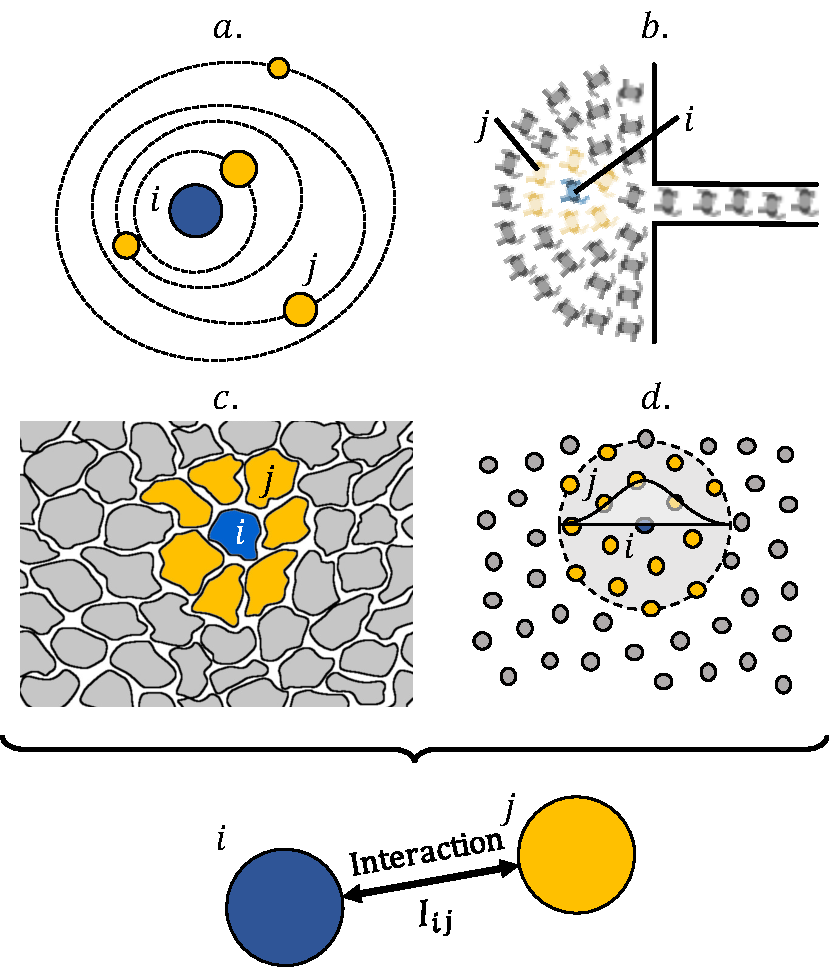
\includegraphics[scale=0.5]{interaction_explain.pdf}
  \centering
  \caption{Explanation of the interaction between nearby objects. a.: a solar system, b.: crowd motion, c.: granular material, d.: continuum substance.}
  \label{fig:interaction_explain}
\end{figure}
The design of Nauticle aims flexible adoption and application of arbitrary interaction laws over a set of spatially distributed particles.


The subsequent sections present how Nauticle subserves the application of particle-based methods.

\subsection{Adoption of interaction laws}
While in Section \ref{sec:usage_of_nauticle} the usage of Nauticle is described, this section specifies how to adopt a new interaction scheme (hereinafter method) formerly not implemented in Nauticle. Since it is inevitable to modify the code, Nauticle requires recompilation to be extended with new methods.

For a better understanding, the implementation process is divided into the steps below, illustrated by the adoption of a user-defined interaction named \textbf{USER\_METHOD}. Here we assume that \textbf{USER\_METHOD} operator has two operands and later it should be referred as \textit{user\_method(operand1, operand2)} in the YAML-configuration file.

\textbf{Step 1: Definition of a child of the interaction class (\textbf{pmInteraction}).} \\
The minimal example of the \textbf{USER\_METHOD} class reads as:
\begin{example}{Class definition}{}
\lstset{basicstyle=\tiny}
\begin{lstlisting}[language=c++]
  class USER_METHOD : public pmInteraction<2> {
  private:
    std::shared_ptr<pmExpression> clone_impl() const override;
  public:
    USER_METHOD() {}
    USER_METHOD(std::array<std::shared_ptr<pmExpression>,2> op);
    USER_METHOD(USER_METHOD const& other);
    USER_METHOD(USER_METHOD&& other);
    USER_METHOD& operator=(USER_METHOD const& other);
    USER_METHOD& operator=(USER_METHOD&& other);
    virtual ~USER_METHOD() {}
    void print() const override;
    pmTensor evaluate(int const& i, size_t const& level=0) const override;
    std::shared_ptr<USER_METHOD> clone() const;
  };
\end{lstlisting}
\end{example}
The key member function of the class is the \textit{evaluate} method:
\begin{example}{evaluate member of \textbf{USER\_METHOD}}{}
\lstset{basicstyle=\tiny}
\begin{lstlisting}[language=c++]
  pmTensor USER_METHOD::evaluate(int const& i, size_t const& level/*=0*/) const {
    if(!this->assigned) { /* No particle system assigned to the USER_METHOD interaction. */ }
    size_t dimension = this->psys.lock()->get_particle_space()->get_domain().get_dimensions();

    pmTensor op1_i = this->operand[0]->evaluate(i,level);
    pmTensor op2_i = this->operand[1]->evaluate(i,level);

    auto lambda = [&](pmTensor const& rji,
                      int const& i, 
                      int const& j, 
                      double const& cell_size, 
                      pmTensor const& bc) ->pmTensor
    {
      pmTensor op1_j = this->operand[0]->evaluate(j,level);
      pmTensor op2_j = this->operand[1]->evaluate(j,level);
      pmTensor contribution{dimension,1,0};
      double d_ji = rel_pos.norm();
      if(d_ji > NAUTICLE_EPS && d_ji < cell_size) {
        contribution += /* Calculate contribution of node j to i. */;
      }
      return contribution;
    };

    // Call iterator method inherited from pmInteraction to process 
    // the summation over the neighbors using the given lambda function.
    return this->interact(i, lambda);
  }
\end{lstlisting}
\end{example}
which is responsible for the evaluation of \textit{user\_method(operand1, operand2)} through the summation of the neighboring particles. The lambda function --- considered to be the core of the interaction --- determines a single interaction between the particle of interest denoted by $i$ and a neighboring particle $j$. There are further supplementary methods to be defined such as constructors, clone functions, and the printer function. Since their definition is straightforward based on the available adoptions, this guide does not specify them in detail. It is strongly recommended to follow the convention of Nauticle and place the header file (either directly or in a subfolder) into the Nauticle \textit{include} directory and a source file if any, to the \textit{src} folder.

\textbf{Step 2: Registration of the \textit{user\_method} function name in the expression parser of Nauticle.} \\
The list of function names (\textbf{list\_of\_functions}) in \textbf{pmMath\_test.cpp} holds the complete collection of functions that can be interpeted by the expression parser. One needs to simply extend the list by the desired function name, in this case \textit{user\_method}. It is also required to manually change the list size in the same file as well as in the class definition of \textbf{pmMath\_test}.

\textbf{Step 3: Extend the expression parser.} \\
To let the expression parser build the tree of expressions including \textit{user\_method}, the \textbf{pmExpression\_parser.cpp} is required to be extended by the declaration of the desired node. This is shown in detail below:
\begin{example}{Declaration of \textbf{USER\_METHOD} node}{}
\lstset{basicstyle=\tiny}
\begin{lstlisting}[language=c++]
  // ...
  } else if(is_function(it)) {
    // ...
    if(it=="user_method") {
      std::array<std::shared_ptr<pmExpression>,2> operands;
      stack_extract(e, operands);
      e.push(std::make_shared<USER_METHOD>(operands));
    }
    // ...
  }
  // ...
\end{lstlisting}
\end{example}
where the array size is identical with the number of operands of \textit{user\_method}.

\textbf{Step 4: Rebuild the executable.} \\
Assuming that the definition of the \textbf{USER\_METHOD} class is placed in a separate source file, the Makefile becomes expired and requires a regeneration by cmake in the main Nauticle directory. After that, Nauticle can be compiled and built executing the command 'make' in the same directory:
\begin{lstlisting}[language=bash]
  $ cmake CMakeLists.txt
  $ make
\end{lstlisting}


After performing the four steps above, Nauticle becomes suitable for the application of the desired interaction by simply referring it in a configuration file:
\begin{example}{Application of the \textit{user\_method} interaction}{}
\lstset{basicstyle=\tiny}
\begin{lstlisting}[language=YAML]
  <!-- ... -->
  <equations>
    <eq1 value="phi=user_method(op1, op2)"/>
  </equations>
  <!-- ... -->
\end{lstlisting}
\end{example}

Note: some of the schemes may require further mutual members, such as kernel functions, in case of schemes like SPH. To avoid repeated declarations of filter functions, a \textbf{pmFilter} class is already implemented in the Nauticle expression tree.


\section{Installation}
Since the Nauticle package currently does not provide a pre-built version, the user is required to build the binaries directly from source code enclosed in the package manually or by means of the automated installation process.
\subsection{Requirements}
Currently, the installation process does not support Windows, it works only on Linux (distributions that support Advanced Packaging Tool (APT)) and Mac OSX systems. Hereinafter Linux is considered to support APT.
Nauticle requires a few dependencies and requirements to be installed. These are the following:
\begin{itemize}
  \item gcc and g++ of version 4.8.
  \item cmake (at least version 3.5) (\myhref{https://cmake.org/download/}{https://cmake.org/download/}),
  \item Visualization Toolkit 7.0.0 (\myhref{http://www.vtk.org/files/release/7.0/VTK-7.0.0.zip}{http://www.vtk.org/files/release/7.0/VTK-7.0.0.zip}),
  \item Common utilities (\myhref{https://bitbucket.org/BalazsToth/commonutils}{https://bitbucket.org/BalazsToth/commonutils}),
  \item ProLog (\myhref{https://bitbucket.org/BalazsToth/prolog}{https://bitbucket.org/BalazsToth/prolog}),
  \item yaml-cpp (\myhref{https://github.com/jbeder/yaml-cpp}{https://github.com/jbeder/yaml-cpp}).
  \item C2C (\myhref{https://bitbucket.org/nauticleproject/c2c}{https://bitbucket.org/nauticleproject/c2c}).
\end{itemize}
The details of the required dependencies are not discussed here, please follow the links to find more information about the listed packages. Further dependencies could be required by the Visualization Toolkit and yaml-cpp.

During the installation process, it is assumed that the user has internet connection and root privileges (super user). Throughout the following subsection, the automatic installation procedure is discussed in detail.
Note: to avoid any version conflicts it is preferred to install and build Nauticle with its dependencies using HashDist, which is an environment management system (\myhref{https://github.com/hashdist/hashdist}{https://github.com/hashdist/ hashdist}). However, it is not mandatory and the automated installation process does not apply any environment manager. \\
Except for the VTK library, all header and binary files related to the dependencies are required to be copied into the /usr/local/include/<dependency> and /usr/local/lib/<dependency> directories in case of both Linux and Mac systems. VTK libary should be placed into the directory /usr/local/VTK.7.0.0 and built simply by following the instructions of the VTK Documentation. Obviously, to compile and build Nauticle, all its dependencies are required to be completely installed in the proper directories.
\subsection{Automated installation}
Although it is possible to install and build the dependencies and Nauticle manually, it is recommended to use the installation shell script arriving with Nauticle. However, it is assumed that the proper version (v4.8) of \texttt{gcc} and \texttt{g++} are already installed. The script installs the whole package including the dependencies by typing the command
\begin{lstlisting}[language=bash]
  $ sh (*@\installer{}@*)
\end{lstlisting}
in terminal after changing directory to the desired folder. The content of the script with explanations is as follows:

\begin{example}{\installer{}}{}
\lstset{basicstyle=\tiny}
\begin{lstlisting}[language=bash]
#!/bin/sh
if [ $(id -u) -eq 0 ]
  then echo "Please do not run as root. I will ask for permissions when necessary."
  exit
fi
# Versions of nauticle and its dependencies
NAUTICLE_version="1.1.190131"
VTK_version="7.0.0"
CU_VERSION="1.0.190131"
PL_version="1.0.190131"
C2_version="1.0.190131"
YAMLCPP_version="0.6.0"

# Set current directory to install directory.
INSTALL_DIR=$PWD
sudo chown ${USER} ${INSTALL_DIR}

# Set OS variable (assume linux)
OS="Linux"
NUM_THREADS=4
if [ "$(uname)" = "Darwin" ]; then
# if mac, install wget, and cmake
    brew install wget
    brew install cmake
    brew install boost
    OS="Mac"
    NUM_THREADS=$(sysctl -n hw.ncpu)
elif [ $OS = "Linux" ]; then
  # if linux, install opengl and cmake
    sudo apt-get update
  sudo apt-get --yes --force-yes install build-essential
  sudo apt-get --yes --force-yes install freeglut3-dev
  sudo apt-get --yes --force-yes install cmake
  sudo apt-get --yes --force-yes install libboost-all-dev
  NUM_THREADS=$(nproc)
fi

echo Setting number of threads for compilation to $NUM_THREADS

# Install proper version of VTK library
wget http://www.vtk.org/files/release/7.0/VTK-$VTK_version.zip
sudo unzip VTK-$VTK_version.zip -d /usr/local/
cd /usr/local/VTK-$VTK_version
sudo cmake .
sudo make -j${NUM_THREADS}

# Go to install directory
cd $INSTALL_DIR

# Download and unzip the required packages
PCKG_CU=commonutils_$CU_VERSION.zip
PCKG_PL=prolog_$PL_version.zip
PCKG_C2=c2c_$C2_version.zip
PCKG_NA=nauticle_$NAUTICLE_version.zip
PCKG_YM=yaml-cpp-$YAMLCPP_version.zip
wget https://bitbucket.org/BalazsToth/commonutils/downloads/$PCKG_CU
wget https://bitbucket.org/BalazsToth/prolog/downloads/$PCKG_PL
wget https://bitbucket.org/nauticleproject/c2c/downloads/$PCKG_C2
wget https://bitbucket.org/nauticleproject/nauticle/downloads/$PCKG_NA
wget https://github.com/jbeder/yaml-cpp/archive/$PCKG_YM
unzip $PCKG_CU
unzip $PCKG_PL
unzip $PCKG_NA
unzip $PCKG_YM
unzip $PCKG_C2
# sudo chmod -R 777 commonutils prolog c2c nauticle yaml-cpp-release-$YAMLCPP_version

# Install the dependencies and the nauticle executable (nauticle) itself
cd $INSTALL_DIR/commonutils
cmake .
cmake .
sudo make install -j${NUM_THREADS}
 
cd $INSTALL_DIR/prolog
cmake .
cmake .
sudo make install -j${NUM_THREADS}

cd $INSTALL_DIR/yaml-cpp-yaml-cpp-$YAMLCPP_version
cmake .
cmake .
sudo make -j${NUM_THREADS}
sudo make install

cd $INSTALL_DIR/c2c
cmake .
cmake .
sudo make install -j${NUM_THREADS}

# Set directory name for executable
BIN_DIR="${INSTALL_DIR}/nauticle/bin/$OS"
cd $INSTALL_DIR/nauticle
cmake .
cmake .
mkdir $BIN_DIR
sudo make install -j${NUM_THREADS}
cd ..

# Add BIN_DIR to the environment PATH variable
if [ "$OS" = "Mac" ]; then
  sudo printf "\nexport PATH=\${PATH}:$BIN_DIR\n" >> ~/.bash_profile
    alias brc='source ~/.bash_profile'
elif [ "$OS" = "Linux" ]; then
  sudo printf "\nexport PATH=\${PATH}:$BIN_DIR\n" >> ~/.bashrc
  alias brc='source ~/.bashrc'
fi

# Generate script file to run nauticle
# (this file is optional and probably useful only when using Nauticle through ssh)
sudo rm -f start.sh
touch start.sh

printf "#!/bin/sh\nshift\nexecutable=$BIN_DIR/nauticle\n" >> start.sh
printf "sudo \$executable \"\$@\"" >> start.sh

# Purge temparay files
while true; do
  read -p "Do you wish to delete temporary files?" yn
    case $yn in
        [Yy]* ) cd $INSTALL_DIR
          sudo rm -r commonutils prolog c2c yaml-cpp-yaml-cpp-$YAMLCPP_version
          sudo rm $PCKG_CU $PCKG_PL $PCKG_YM $PCKG_NA $PCKG_C2 VTK-$VTK_version.zip
          mv $BIN_DIR/nauticle $INSTALL_DIR/tmp
          sudo rm -rf nauticle
          mkdir -p "$BIN_DIR"
          mv $INSTALL_DIR/tmp $BIN_DIR/nauticle
          break;;
        [Nn]* ) exit;;
        * ) echo "Please answer yes or no.";;
    esac
done
\end{lstlisting}
\end{example}

It downloads and builds the necessary files into your system. After installation, the executable (\execname{}) is placed in the bin directory and the \textbf{start.sh} file is generated in the installation directory. The installer also adds the bin directory to your environment variables, therefore you can run Nauticle from different directories by simply typing \textbf{nauticle} in terminal. To activate this feature it may be necessary to manually reload the \textbf{.bash\_profile} or \textbf{.bashrc} file in your home directory using the \texttt{source} command.
In certain cases, when the environment variables are not available you can perform computations using the \textbf{start.sh} file in the simulation folder:
\begin{lstlisting}[language=bash]
  $ sh start.sh
\end{lstlisting}
Note that the optional runtime commands are forwarded by \textbf{start.sh}, which supports the execution of
\begin{lstlisting}[language=bash]
  $ sh start.sh <arguments_list>
\end{lstlisting}
where the arguments\_list consists of the options listed in Table \ref{tbl:runtime_commands}.

To uninstall Nauticle, users only need to run the attached \texttt{uninstall.sh} script that wipes all the installed include and library files. However, since the dependencies (c2c, prolog, commonutils) may have other packages depending on them, they need to be removed separately but in the same way.

\section{Examples} \label{sec:examples}
This section describes a few examples of the application of the Nauticle solver to more or less simple physical models governed by partial or ordinary differential equations. The examples are selected to cover a wide range of applications from both physical and mathematical point of view. For further simulation examples, the reader is encouraged to study the \textit{undocumented examples} attached to the Nauticle package.

Note that the solutions presented in this section might have further different, but also correct realizations.
\subsection{Couette-flow}
\subsubsection{Problem definition}
One of the simplest and most frequently investigated fundamental test cases in fluid mechanics is the laminar Couette-flow. The upper one of the two infinite sized parallel walls shown in Figure \ref{fig:couette} is moving in $y$ direction with velocity $v=1$m/s.
\begin{figure}[H]
  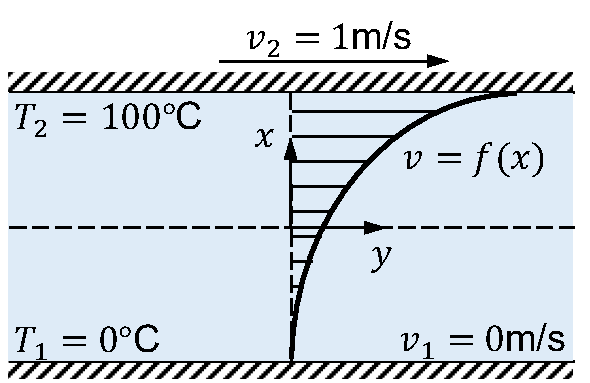
\includegraphics[scale=0.7]{couette.pdf}
  \centering
  \caption{Temperature-dependent laminar Couette-flow between parallel walls.}
  \label{fig:couette}
\end{figure}\vspace*{3pt}
The walls have different temperatures $T_1=0^\circ$C and $T_2=100^\circ$C affecting the fluid temperature and consequently the kinematic viscosity $\nu$ by the
\begin{equation}
\nu(T)=\nu_0 \exp(-bT)
\end{equation}
formula. The constants here are chosen to be $\nu_0=0.1\rm{m}^2/\rm s$ and $b=0.03 ^\circ C^{-1}$. Since the flow is laminar, the temperature distribution between the parallel walls can be determined by the heat equation
\begin{equation} \label{eq:couette_laplace}
\frac{\partial T}{\partial t}=\lambda\Delta T,
\end{equation}
where $\lambda=0.01$ is the heat conduction coefficient. The fluid velocity in the channel is governed by 
\begin{equation} \label{eq:couette_eom}
\frac{\partial v}{\partial t}=\nabla(\nu(T)\nabla v),
\end{equation}
where $v$ is the fluid velocity field. The problem is stationary and one-dimensional, therefore equations \equref{eq:couette_laplace} and \equref{eq:couette_eom} can be simplified as
\begin{flalign} \label{eq:couette_simplified}
\begin{split}
&\frac{d^2T}{dx^2}=0, \\
&\frac{d}{dx}\bigg(\nu(T)\frac{dv}{dx}\bigg)=0.
\end{split}
\end{flalign}
Applying Dirichlet boundary conditions to both the temperature and velocity fields:
\begin{flalign} \label{eq:couette_bc}
\begin{split}
&T(-L/2)=0,\\
&T(L/2)=100, \\
&v(-L/2)=0, \\
&v(L/2)=1, \\
\end{split}
\end{flalign}
where $L=1$m is the width of the channel, the solution of \equref{eq:couette_simplified} can be constructed analytically:
\begin{flalign} \label{eq:couette_analytical}
\begin{split}
&T(x)=\frac{T_2-T_1}{L}x+\frac{T_1+T_2}{2}=100x+50,\\
&v(x)=\frac{v_2-v_1}{e^{bT_1}-e^{bT_2}}(e^{bT(x)}-e^{bT_1})+v_1=\frac{e^{b(100x+50)}-1}{e^{100b}}.\\
\end{split}
\end{flalign}

\subsubsection{Numerical model and results}
To solve the Couette-flow problem the simplest model is built in Nauticle using the SPH collocation scheme. Although SPH is Lagrangian (particles should follow material trajectories), in the case of laminar parallel flow, the movement of particles can be omitted due to the identity of the Lagrangian and Eulerian fields. The time dependent discretized system of equations is
\begin{flalign} \label{eq:couette_sph_discretized}
\begin{split}
&\frac{dT_i}{dt}=\lambda\sum_j{2(T_j-T_i)\frac{1}{\textbf{r}_{ji}}\frac{m_j}{\rho_j}\nabla W_{ij}}, \\
&\frac{dv_i}{dt}=\sum_j{(\nu_j+\nu_i)(v_j-v_i)\frac{1}{\textbf{r}_{ji}}\frac{m_j}{\rho_j}\nabla W_{ij}}. \\
\end{split}
\end{flalign}
After the discretization the YAML-document can be constructed:
\begin{example}{Couette-flow configuration file}{}
\lstset{basicstyle=\tiny}
\begin{lstlisting}[language=YAML]
simulation: 
  case: 
    workspace: 
      constants: 
        - L: 1
        - csize: L/20
        - dx: csize/2
        - rho0: 1000
        - mass: dx*rho0
        - lambda: 0.01
        - nu0: 0.1
        - b: 0.03
        - T1: 0
        - T2: 100
        - v1: 0
        - v2: 1
      variables: 
        - dt: 0.001
        - Time: 0
      particle_system: 
        domain: 
          cell_size: csize
          minimum: -L/csize/2-1
          maximum: L/csize/2+1
          boundary: periodic
        grid: 
          gid: 1
          gpos: -L/2-csize+dx/2
          gsize: csize
          goffset: 0
          gip_dist: dx
        grid: 
          gid: 0
          gpos: -L/2+dx/2
          gsize: L-dx
          goffset: 0
          gip_dist: dx
        grid: 
          gid: 2
          gpos: L/2-dx/2
          gsize: csize
          goffset: 0
          gip_dist: dx
      fields: 
        - a: 0
        - v: if(eq(0,gid),0,if(eq(gid,1),v1,v2))
        - T: if(eq(0,gid),0,if(eq(gid,1),T1,T2))
        - T_dot: 0
        - nu: 0.1
    equations: 
      - time: Time=Time+dt
      - heat: T_dot=lambda*sph_L0(T,mass,rho0,Wp32210,csize)
        condition: eq(gid,0)
      - temp: T=euler(T,T_dot,dt)
        condition: eq(gid,0)
      - viscosity: nu=nu0*exp(-b*T)
      - moment: a=sph_L1(nu,v,mass,rho0,Wp32210,csize)
        condition: eq(gid,0)
      - vel: v=euler(v,a,dt)
        condition: eq(gid,0)
  parameter_space: 
    simulated_time: 100
    print_interval: 1
    confirm_on_exit: false
    output_format: BINARY
    compile_case: true
\end{lstlisting}
\end{example}
Since the initial conditions for both the temperature and velocity are uniform, the solution of the discretized equations needs to be repeated until the result is sufficiently formed. In this case the simulated time is $100$ s. The final result is compared with the analytical solution in Figure \ref{fig:couette_results}.
\begin{figure}[H]
  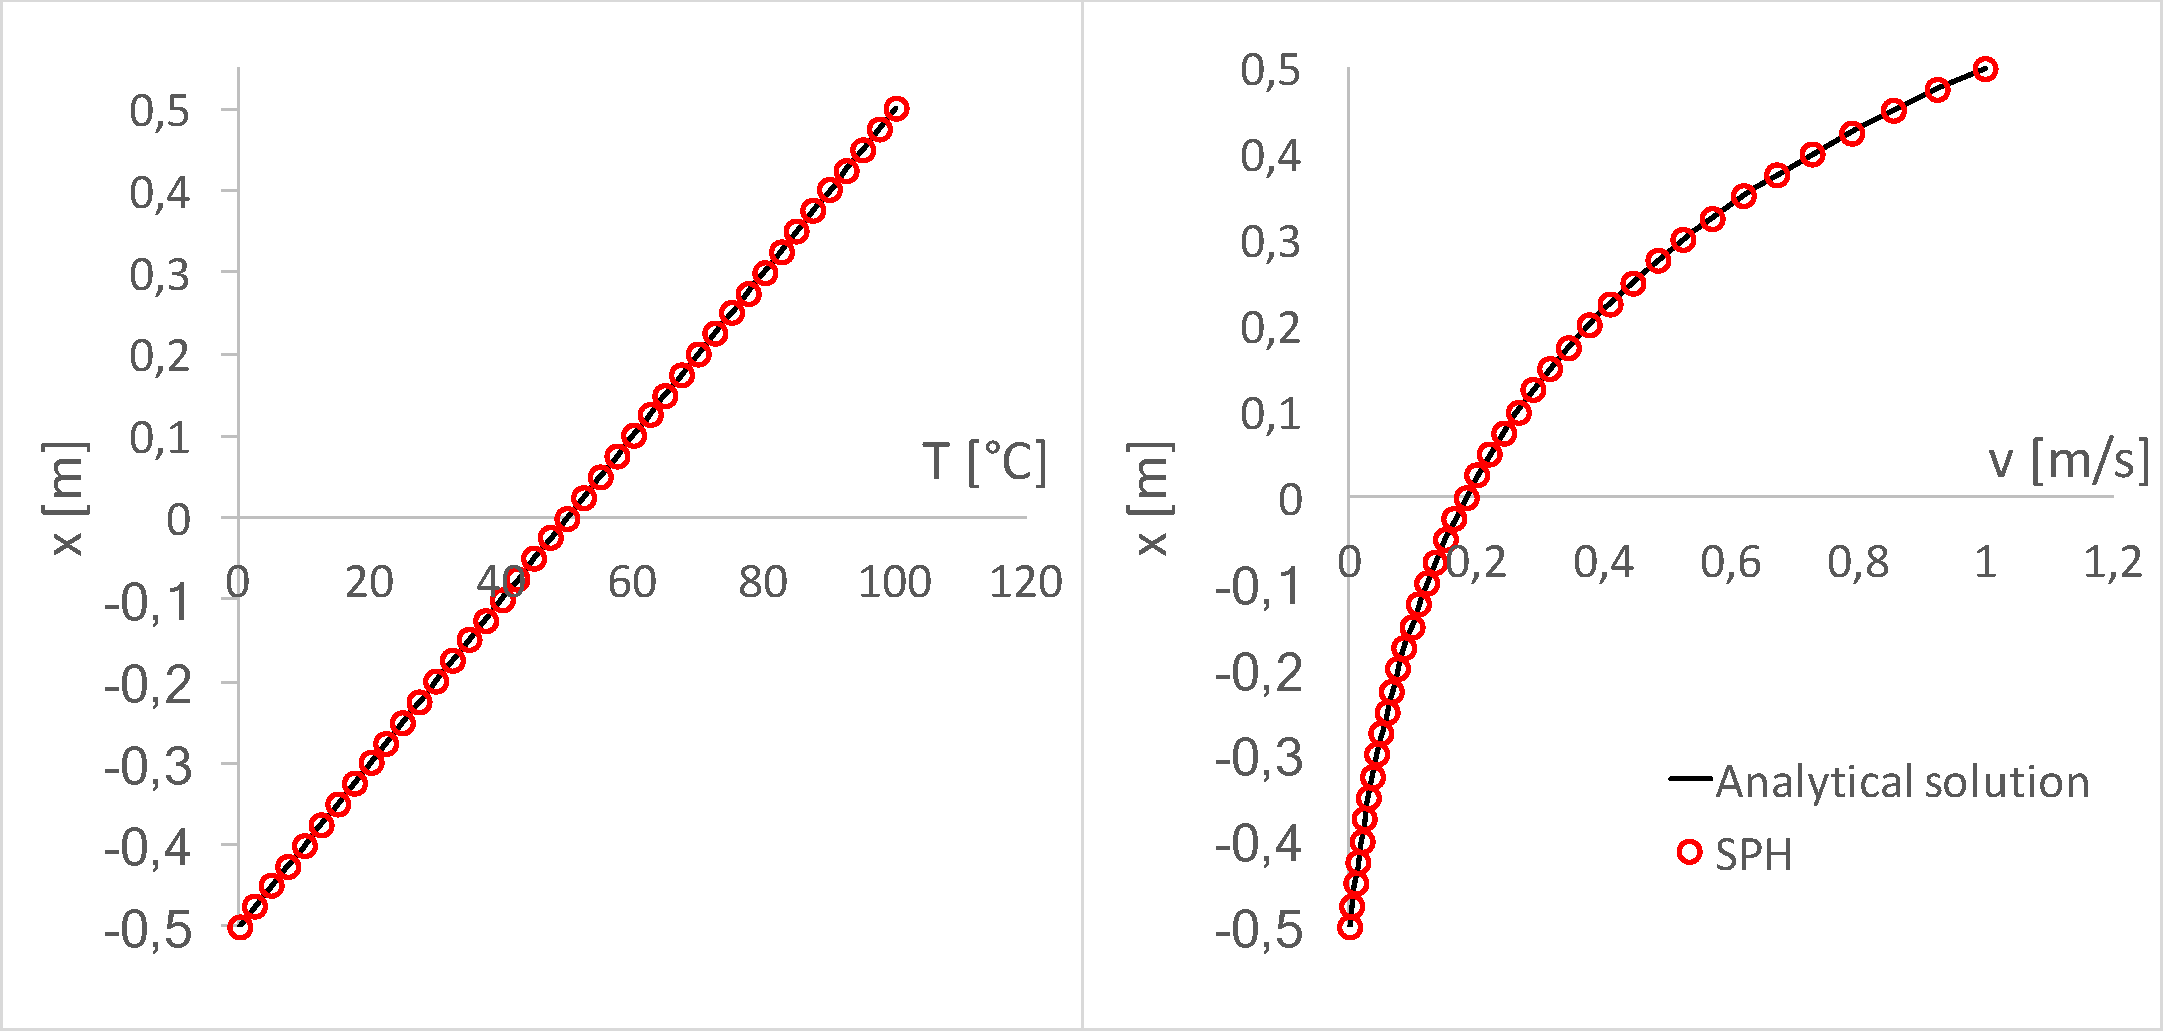
\includegraphics[scale=0.4]{couette_result.pdf}
  \centering
  \caption{Couette-flow results comparison.}
  \label{fig:couette_results}
\end{figure}\vspace*{3pt}

The results show very good agreement with the analytical solution in case of both the linear temperature and the exponential velocity distributions.
\subsection{Phase separation on a sphere} \label{sec:cahn_hilliard}
\subsubsection{Problem definition}
The process of the separation of two phases is usually modelled by the fourth order nonlinear Cahn-Hilliard equation
\begin{flalign} \label{eq:cahnhilliard}
\begin{split}
&\frac{\partial c}{\partial t}=D\Delta \mu,\\
&\mu=c^3-c-\gamma\Delta c, \\
\end{split}
\end{flalign}
where $c\in[-1,1]$ is the phase concentration, $\mu$ is the chemical potential, $\sqrt{\gamma}$ is the thickness of the transition region between the two phases and $D$ is a diffusion coefficient. In this particluar case the solution of equation \equref{eq:cahnhilliard} is investigated over a surface of a sphere.

\subsubsection{Numerical model and results}
The numerical scheme to discretize the system \equref{eq:cahnhilliard} is chosen to be SPH. Since the geometry is generated in Cartesian coordinates, the domain itself is three-dimensional. However, the mollifier in the spatial interpolant should be two-dimensional due to the fact, that the problem is interpreted on a spherical surface. The discretized form of the equations \equref{eq:cahnhilliard} are
\begin{flalign} \label{eq:cahnhilliard_sph_discretized}
\begin{split}
&\frac{\partial c_i}{\partial t}=D\sum_j{2(\mu_j-\mu_i)\frac{m_j}{\rho_j}\nabla W_{ij}},\\
&\mu_i=c^3-c-\gamma\sum_j{2(c_j-c_i)\frac{m_j}{\rho_j}\nabla W_{ij}}, \\
\end{split}
\end{flalign}
where again, $W_{ij}$ is normalized in two dimensions. The configuration file to solve \equref{eq:cahnhilliard_sph_discretized} is
\begin{example}{Cahn-Hilliard configuration file}{}
\lstset{basicstyle=\tiny}
\begin{lstlisting}[language=YAML]
simulation:
  case:
    workspace:
      constants:
        - L: 2
        - dx: 0.0675
        - csize: dx*2.1
        - rho0: 1000
        - mass: dx^2*rho0
        - D: 0.003
        - CFL: 0.1
        - gamma: (csize/3)^2
        - dt_g: gamma/csize^2
      variables:
        - dt: 0.003
        - Time: 0
        - print_interval: dt
      particle_system:
        domain:
          cell_size: csize|csize|csize
          minimum: -15|-15|-15
          maximum: 15|15|15
          boundary: 0|0|0
        grid:
          gid: 0
          file: points.xyz
      fields:
        - c: rand(-1,1)
        - c_dot: 0
        - mu: 0
    equations:
      - time: Time=Time+dt
      - chemical_potential: mu=c^3-c-gamma*sph_L0(c,mass,rho0,Wp32220,csize)
      - Cahn_Hilliard: c_dot=D*sph_L0(mu,mass,rho0,Wp32220,csize)
      - integration: c=euler(c,c_dot,dt)
      - new_dt: dt=CFL*min(1/fmax(c_dot),dt_g)
  parameter_space:
    simulated_time: 150
    print_interval: exp(Time/45)
    confirm_on_exit: false
    output_format: BINARY
    compile_case: true
\end{lstlisting}
\end{example}
The phase separation process has a decaying intensity in the function of time, therefore the printing interval is adaptively modified with an exponential law to minimize the amount of simulation result files and keep the temporal sampling appropriate at the same time. The evolution of phase separation is shown in Figure \ref{fig:cahnhilliard_result} by the triangulation of the surface.
\begin{figure}[H]
  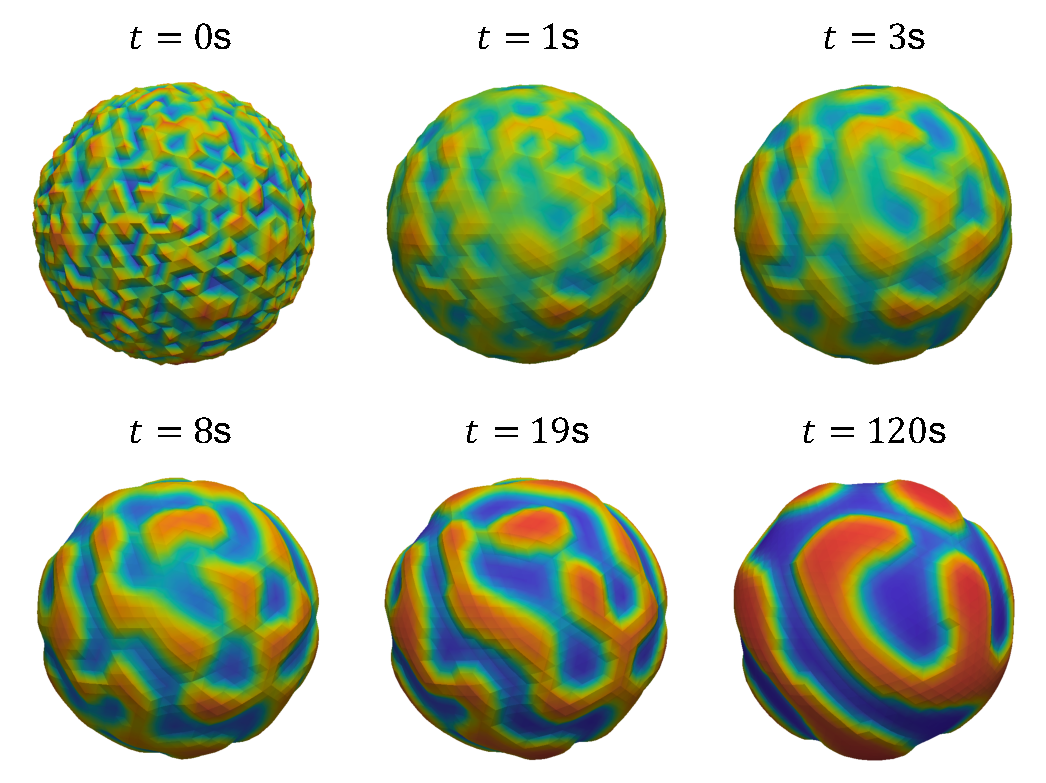
\includegraphics[scale=0.6]{cahnhilliard_result.pdf}
  \centering
  \caption{Evolution of phases on the sphere.}
  \label{fig:cahnhilliard_result}
\end{figure}\vspace*{3pt}


\subsection{Particle damper}
Particle dampers are one of the widely investigated damper systems today. Although there exist several analytical models to design and scale a particle damper, the complexity of the problem still requires experimental and numerical investigation. The geometry of the tank, the number, and sizes of particles, the materials, the operating frequency are only some of the huge amount of possibilities concerning the development of particle dampers.
\subsubsection{Problem definition}
This test case simulates a simple three-dimensional oscillating cubic tank filled with spheres of identical radii. The tank is initially at rest in the position $z_0=-0.05$ m. The layout of the particle damper is presented in Figure \ref{fig:particle_damper_geom}, furthermore the values of the introduced quantities are summarized in Table \ref{tbl:particle_damper_values}. The system is supported by the ideal linear spring merely damped by the collision of the included set of spheres.
\begin{figure}[H]
  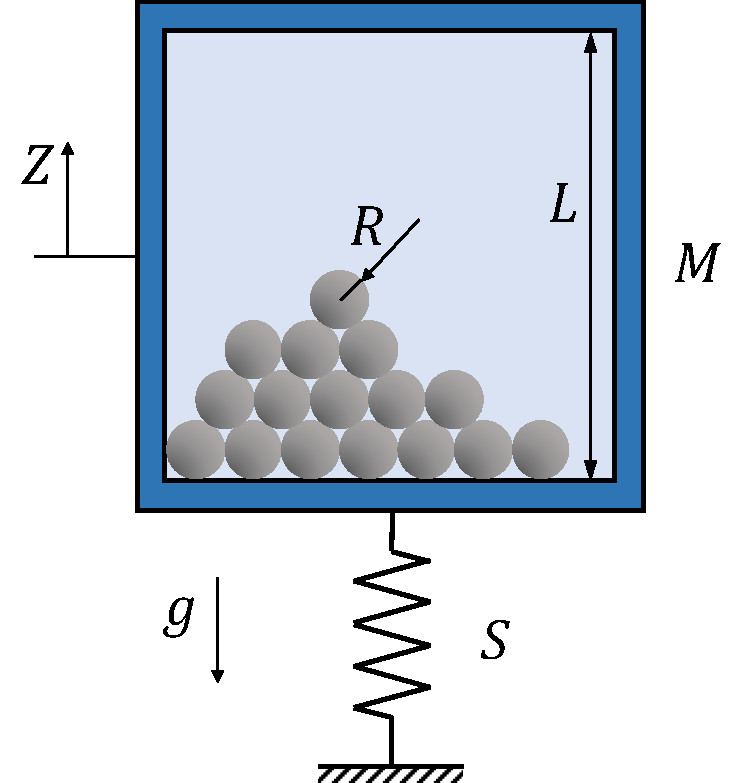
\includegraphics[scale=0.4]{particle_damper_geom.pdf}
  \centering
  \caption{Physical layout of the particle damper.}
  \label{fig:particle_damper_geom}
\end{figure}\vspace*{3pt}
\begin{table}[H]
\begin{center}
\caption{Parameters of the particle damper simulation.}\label{tbl:particle_damper_values}
\begin{tabular}{ c l r } 
\toprule[1.5pt]
\bf Name & \bf Description & \bf Value \\
\midrule
$M$ & Tank mass & $20$ kg \\
$s$ & Spring stiffness & $78956.8$ kg/s$^2$ \\
$R$ & Particle radius & $4$ mm \\
$L$ & Tank edge length & $0.1$ m \\
$\rho$ & Particle mass & $7850$ kg/m$^3$ \\
$E$ & Particle Young modulus & $2.06$ MPa \\
$\nu$ & Particle Poisson's ratio & $0.33$ \\
$g$ & Gravitational acceleration & $-9.81$ m/s${^2}$ \\
$N$ & Number of particles & 567 \\
\bottomrule[1.25pt]
\end{tabular}
\end{center}
\end{table}
The one-dimensional equation of motion of the tank is
\begin{flalign} \label{eq:tank_ode}
\begin{split}
M\ddot{Z}+SZ=F^b, \\
F^b = -\bigg[\sum_i{f^b_i}\bigg]^z
\end{split}
\end{flalign}
where $F(t)$ is the resultant of the particle-boundary forces $f^b_i$. The latter appears in the equation of motion of the particles:
\begin{flalign} \label{eq:spheres_ode}
\frac{d^2\textbf{r}_i}{dt^2}=\frac{\textbf{F}^c_i}{m_i}+\frac{\textbf{F}^b_i}{m_i}+\textbf{g},
\end{flalign}
where $\textbf{F}^c$ and $\textbf{F}^b$ are the particle-particle and particle-wall collision forces respectively.
\subsubsection{Numerical model and results}
A simple representaion of the three-dimensional physical model is introduced in this section with the notation that other valid solutions are also possible. To simplify the model and omit the tank the simulation domain is chosen to be the interior of the tank. Since the domain is fixed, this assumption means that the simulation of the particle motion and collision is interpreted in the moving coordinate system associated to the tank and the excitation of the particles is governed purely by a time-dependent acceleration field superposed with the gravitational acceleration. The boundaries of the domain are set to be symmetric, which plays an important role in the calculation of the forces acting on the tank. For the sake of simplicity the angular momentum of the particles is neglected. The solution of the homogeneous part of \equref{eq:tank_ode} is the harmonic function
\begin{flalign} \label{eq:tank_sol}
Z(t)=C_1sin(\gamma t)+C_2cos(\gamma t),
\end{flalign}
where $C_1$ and $C_2$ are constants depending on the initial conditions and $\gamma^2=S/M$. Due to the lack of damping, the oscillation has constant amplitude. The particles' motion is determined by \equref{eq:spheres_ode} written as
\begin{flalign} \label{eq:spheres_ode_full}
\frac{d^2\textbf{r}_i}{dt^2}=\frac{\textbf{F}^c_i}{m_i}+\frac{\textbf{F}^b_i}{m_i}+\textbf{g}=\frac{1}{m_i}\sum_j{\textbf{f}^c_i(\textbf{r}_{ji},v_{ji},...)}+\frac{\textbf{F}^b_i}{m_i}+\textbf{g},
\end{flalign}
where $f^c$ denotes the collection of the collision laws introduced in Section \ref{sec:DEM_intro}. The second term on the RHS of \equref{eq:spheres_ode} operates with the same collision laws at the symmetric boundaries, which in turn contributes to \equref{eq:tank_ode}.
During the simulation the tank position, velocity and acceleration has to be calculated at each time steps. These quantities are considered as variables and calculated by the numerical solution of \equref{eq:tank_ode}. The configuration file for the particle damper problem is as follows:
\begin{example}{Particle damper configuration file}{}
\lstset{basicstyle=\tiny}
\begin{lstlisting}[language=YAML]
simulation:
  case:
    workspace:
      constants:
        - L: 0.1
        - csize: 0.01
        - R: 0.004
        - mass: 7850*4/3*R^3*pi
        - E: 2.06e6
        - nu: 0.33
        - M: 20
        - freq: 10
        - gamma: 10*2*pi
        - S: gamma^2*M
        - g: 0|0|-9.81
      variables:
        - T: 0
        - dt: 5e-4
        - A: 0
        - V: 0
        - Z: -0.05
      particle_system:
        domain:
          cell_size: csize|csize|csize
          minimum: -L/2/csize|-L/2/csize|-L/2/csize
          maximum: L/2/csize|L/2/csize|L/2/csize
          boundary: symmetric|symmetric|symmetric
        grid:
          gid: 0
          gpos: -9*R|-9*R|-L/2
          gsize: 18*R|18*R|14*R
          goffset: R|R|R
          gip_dist: 2*R|2*R|2*R
      fields:
        - a: 0|0|0
        - v: rand(-0.2,0.2)|rand(-0.2,0.2)|rand(-0.2,0.2)
        - om: 0|0|0
        - bottom: Z-0.05
        - top: Z+0.05
    equations:
      - time: T=T+dt
      - eq: a=dem_l(v,om,R,mass,E,nu,0.1)/mass
      - tank_acceleration: A=(-transpose(fsum(a)*mass)*e_k-S*Z)/M
      - iv: v=euler(v,a+g-A*e_k,dt)
      - ia: r=euler(r,v,dt)
      - tank_velocity: V=euler(V,A,dt)
      - tank_position: Z=euler(Z,V,dt)
      - bottom: bottom=Z-0.05
      - top: top=Z+0.05
  parameter_space:
    simulated_time: 1
    print_interval: 10*dt
    confirm_on_exit: 0
    output_format: ASCII
    compile_case: true
\end{lstlisting}
\end{example}
After running the configuration file in Nauticle the individual particle elevations are visualized in Figure \ref{fig:particle_damper_result} together with the bottom and top positions of the tank.
\begin{figure}[H]
  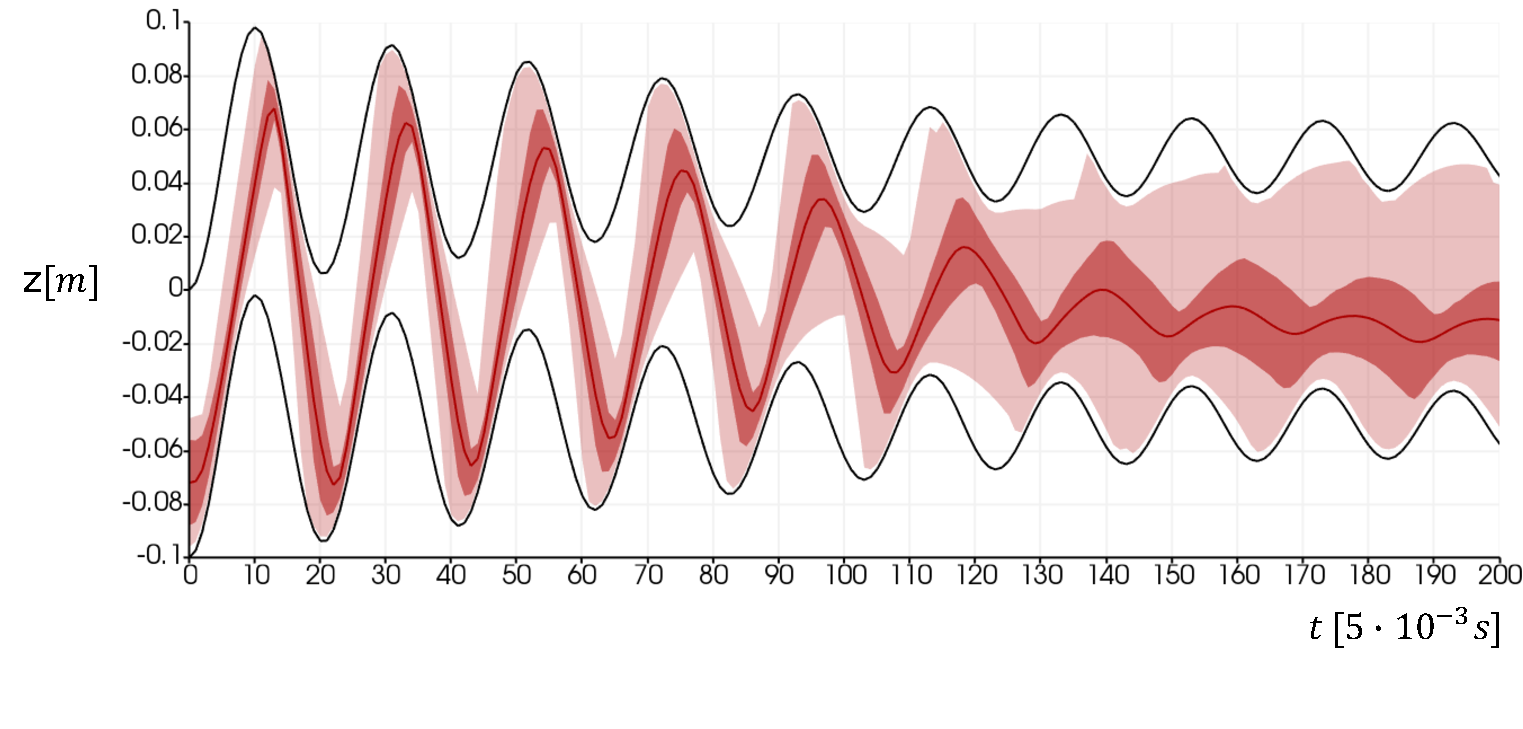
\includegraphics[scale=0.6]{particle_damper_time_series.pdf}
  \centering
  \caption{Elevation of particles (red) and the tank (black) in the function of time.}
  \label{fig:particle_damper_result}
\end{figure}\vspace*{3pt}
As it can be seen the oscillation amplitude is being reduced significantly until the particles start to gather at the bottom due to the smaller peak acceleration.


\subsection{Breaking of free jet} \label{sec:DVM_example}
\subsubsection{Problem definition}
This section provides a simple test case of the break of two-dimensional parallel shear layers generated by a free jet of infinite length. The flow is considered to be inviscid and free of vorticity sources resulting in the exact conservation of vorticity:
\begin{flalign} \label{eq:vorticity_constant}
\frac{d\omega}{dt}=\frac{\partial\omega}{\partial t}+\textbf{v}\nabla\omega=0.
\end{flalign}
Due to its mathematical background, the fulfillment of constraint \equref{eq:vorticity_constant} is simply feasible using the Discrete Vortex Method presented in \ref{sec:DVM}.
\subsubsection{Numerical model and results}
The shear layer on the edges of the free jet are resolved by a set of point vortices with opposite signs along the two edges as drawn in Figure \ref{fig:shear_geom}.
\begin{figure}[H]
  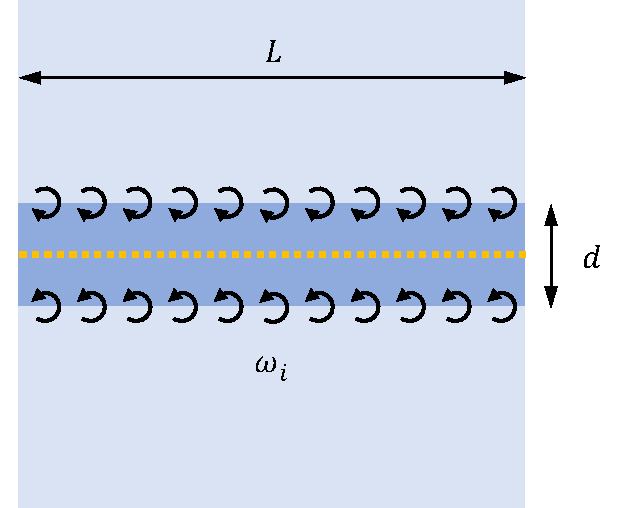
\includegraphics[scale=0.6]{shear_geom.pdf}
  \centering
  \caption{Free jet (dark blue) represented by a series of point vortices along the shear layers. Yellow dots mark the tracer particles. }
  \label{fig:shear_geom}
\end{figure}\vspace*{3pt}
Since the free jet is assumed to be infinite, a periodic boundary has been chosen in streamwise direction to simulate a $L=5$ m long section of the jet. Obviously, the simulated length affects the maximum size of the developing flow structures. The length $5$ m and the number of vortex points are sufficiently large to resolve the process of jet-breaking. To capture the actual physical instability it is inevitable to apply a small initial perturbation on the vortex positions. Such a perturbation could be a sinusoidal shift in spanwise direction with a small amplitude $10^{-6}$ m and wavelength $L/5$ m.

\begin{figure}[H]
  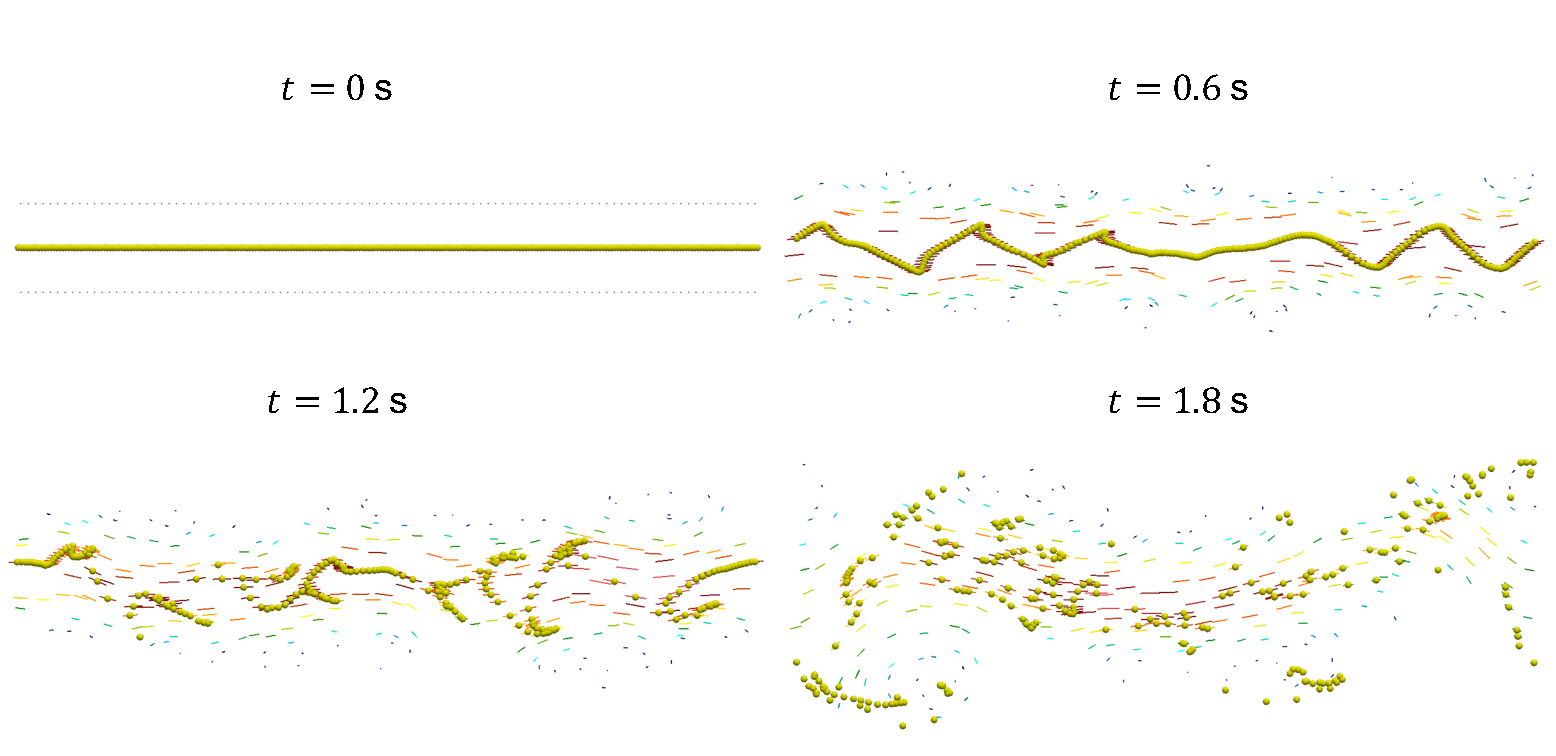
\includegraphics[scale=0.6]{shear_result.pdf}
  \centering
  \caption{Free jet breaking within periodic boundaries. Lines denote velocity vectors of point vortices colored by the velocity magnitude. Yellow spheres are weightless particles tracked through the velocity field induced by the set of point vortices. }
  \label{fig:shear_result}
\end{figure}\vspace*{3pt}

\begin{table} [H]
\begin{center}
\caption{Parameters of the free jet simulation.}\label{tbl:shear_layer_values}
\begin{tabular}{ c l r } 
\toprule[1.5pt]
\bf Name & \bf Description & \bf Value \\
\midrule
$L$ & Simulated length of the jet & $5$ m \\
$\omega_i$ & Vorticity strength of each point vortex & $0.3$ 1/s \\
$d$ & Width of the jet & $0.6$ m \\
$\Delta x$ & Distance between adjacent vortices & $0.05$ m \\
$N_v$ & Number of point vortices & $200$ \\
$N_t$ & Number of tracer particles & $250$ \\
\bottomrule[1.25pt]
\end{tabular}
\end{center}
\end{table}

The simulation is executed using the configuration file below:
\begin{samepage}
\begin{example}{Shear layer configuration file}{}
\lstset{basicstyle=\tiny}
\begin{lstlisting}[language=YAML]
simulation:
  case:
    workspace:
      constants:
        - L: 5
        - c_s: L/2
        - dx: L/50
        - omega: 0.3
        - eps: c_s/30
      variables:
        - T: 0
        - dt: 0.02
      particle_system:
        domain:
          cell_size: c_s|c_s
          minimum: 0|0
          maximum: L/c_s|L/c_s
          boundary: periodic|symmetric
        grid:
          gid: -1 # Bottom vortex pattern
          gpos: 0|L/2-3*dx-dx/2
          gsize: L|dx
          goffset: 0|0
          gip_dist: dx/2|dx
        grid:
          gid: 0 # Tracer particles
          gpos: 0|L/2-dx/2
          gsize: L|dx
          goffset: 0|0
          gip_dist: dx/5|dx
        grid:
          gid: 1 # Top vortex pattern
          gpos: 0|L/2+3*dx-dx/2
          gsize: L|dx
          goffset: 0|0
          gip_dist: dx/2|dx
      fields:
        - w: gid*omega
          symmetric: false
        - v: 0|0
        - noise: sin(elem(r,0,0)*25/pi)*dx*1e-2*e_j
    equations:
      - initial_noise: r=r+noise
        condition: eq(T,0)
      - time: T=T+dt
      - velocity: v=dvm(w,eps)
      - integrate: r=euler(r,v,dt)
  parameter_space:
    simulated_time: 1.8
    print_interval: dt
    confirm_on_exit: 0
    output_format: ASCII
    compile_case: true
\end{lstlisting}
\end{example}
\end{samepage}
As it was pointed out earlier in Section \ref{sec:boundaries}, the physically correct reflection of vorticity and velocity at symmetric boundaries is different. Hence in this example the vorticity field is marked as non-symmetric in the configuration file.


\subsection{Simulation of the Solar System}
The simulation of the Solar System is a typical case of the n-body problem. The size of the objects are negligible and all objects are in interaction with all the others, consequently, the equation of motion \equref{eq:nbody_eom} stands for all objects.
Due to the space-time scale of the Solar System it is recommended to deviate from SI units to decrease the inaccuracy of floating point arithmetics. Here the unit mass is equal to the mass of Earth (am), the unit distance is considered as the average distance of the Sun and the Earth (al) and finally, the unit length of time is one Earth-day (at). These units are summarized in Table \ref{tbl:astronomical_units}.
\begin{table} [H]
\begin{center}
\caption{Units in the Solar System simulation.}\label{tbl:astronomical_units}
\begin{tabular}{ l r r }
\toprule[1.5pt]
\bf Name & \bf Unit & \bf Value \\
\midrule
Mass & am & $5.97\cdot 10^{24}$ kg \\
Distance & al & $1.48093\cdot 10^{11}$ m \\
Time & at & $86400$ s \\
\bottomrule[1.25pt]
\end{tabular}
\end{center}
\end{table}
Hence the gravitational constant is obtained as $\gamma=9.16324149\cdot 10^{-10}\rm{al}^3/(\rm{am}\cdot \rm{at}^2)$. Following \cite{Arminjon2002}, the initial conditions of the Solar System are set to its state at 26 February 2000 00:00 (in heliocentric coordinates) introduced in Table \ref{tbl:solarsystempos} and \ref{tbl:solarsystemvel}. 
\begin{table} [H]
\begin{center}
\caption{Mass of the Solar System planets.}\label{tbl:solarsystemmass}
\begin{tabular}{ l r }
\toprule[1.5pt]
\bf Object & \bf Mass [am] \\
\midrule
Sun & $3.32965046E+05$ \\
Mercury & $5.52604794E-02$ \\
Venus & $8.14805143E-01$ \\
Earth & $1.00000000E+00$ \\
Mars & $1.07447770E-01$ \\
Jupiter & $3.17831793E+02$ \\
Saturn & $9.51620463E+01$ \\
Uranus & $1.45359582E+01$ \\
Neptune & $1.71471140E+01$ \\
Pluto & $2.19381947E-03$ \\
\bottomrule[1.25pt]
\end{tabular}
\end{center}
\end{table}

\begin{table} [H]
\begin{center}
\caption{Positions of the Solar system planets.}\label{tbl:solarsystempos}
\begin{tabular}{ l r r r }
\toprule[1.5pt]
\bf Object & \multicolumn{3}{c}{\bf Position [al]} \\
\midrule
Sun & $0.00000000E+00$  &  $0.00000000E+00$  &  $0.00000000E+00$ \\
Mercury & $-2.52875447E-01$  &  $1.89224913E-01$  &  $1.27303389E-01$ \\
Venus & $1.76553728E-02$  &  $-6.69151143E-01$  &  $-3.02159352E-01$ \\
Earth & $-9.18428887E-01$  &  $3.62942965E-01$  &  $1.57355594E-01$ \\
Mars & $1.21524135E+00$  &  $7.34458249E-01$  &  $3.04013819E-01$ \\
Jupiter & $3.77100459E+00$  &  $3.08343707E+00$  &  $1.22979557E+00$ \\
Saturn & $6.22706292E+00$  &  $6.43146103E+00$  &  $2.38855445E+00$ \\
Uranus & $1.47277740E+01$  &  $-1.24945774E+01$  &  $-5.68075252E+00$ \\
Neptune & $1.71271712E+01$  &  $-2.31196703E+01$  &  $-9.88938537E+00$ \\
Pluto & $-9.80572133E+00$  &  $-2.83258746E+01$  &  $-5.88297808E+00$ \\
\bottomrule[1.25pt]
\end{tabular}
\end{center}
\end{table}

\begin{table} [H]
\begin{center}
\caption{Velocities of the Solar system planets.}\label{tbl:solarsystemvel}
\begin{tabular}{ l r r r }
\toprule[1.5pt]
\bf Object & \multicolumn{3}{c}{\bf Velocity [al/at]} \\
\midrule
Sun & $0.00000000E+00$  &  $0.00000000E+00$  &  $0.00000000E+00$ \\
Mercury & $-2.46358641E-02$  &  $-1.86902265E-02$  &  $-7.42852534E-03$ \\
Venus & $2.02895362E-02$  &  $8.45044680E-04$  &  $-9.03879795E-04$ \\
Earth & $-7.15783449E-03$  &  $-1.47042339E-02$  &  $-6.37503091E-03$ \\
Mars & $-7.19683749E-03$  &  $1.17815694E-02$  &  $5.59840572E-03$ \\
Jupiter & $-5.13821923E-03$  &  $5.54945851E-03$  &  $2.50386823E-03$ \\
Saturn & $-4.47179956E-03$  &  $3.42854338E-03$  &  $1.60843860E-03$ \\
Uranus & $2.67440395E-03$  &  $2.51272963E-03$  &  $1.06268844E-03$ \\
Neptune & $2.59474895E-03$  &  $1.69891959E-03$  &  $6.30906866E-04$ \\
Pluto & $3.06493917E-03$  &  $-1.12260841E-03$  &  $-1.27466162E-03$ \\
\bottomrule[1.25pt]
\end{tabular}
\end{center}
\end{table}
The simulation can be run using the configuration file below:
\begin{samepage}
\begin{example}{Solar system configuration file}{}
\lstset{basicstyle=\tiny}
\begin{lstlisting}[language=YAML]
simulation:
  initial_condition:
    file: solar_system.vtk # Read initial conditions from file
  parameter_space:
    simulated_time: 365.25*1000 # Simulate 1000 years
    print_interval: 365.25 # Print results in every year
    confirm_on_exit: 0
    output_format: ASCII
    compile_case: true
\end{lstlisting}
\end{example}
\end{samepage}
Instead of defining of the particle positions in the configuration file it reads the data and the equations from the VTK file \textbf{solar\_system.vtk}. However, some parameters like the printing interval or the total simulation time is still need to be defined in the configuration file.
Theoretically, the total amount of energy in the Solar system remains constant, at least over the simulated 1000-year period. The sum of the kinetic and potential energy of all planets is plotted in Figure \ref{fig:solar_system_energy}.
\begin{figure}[H]
  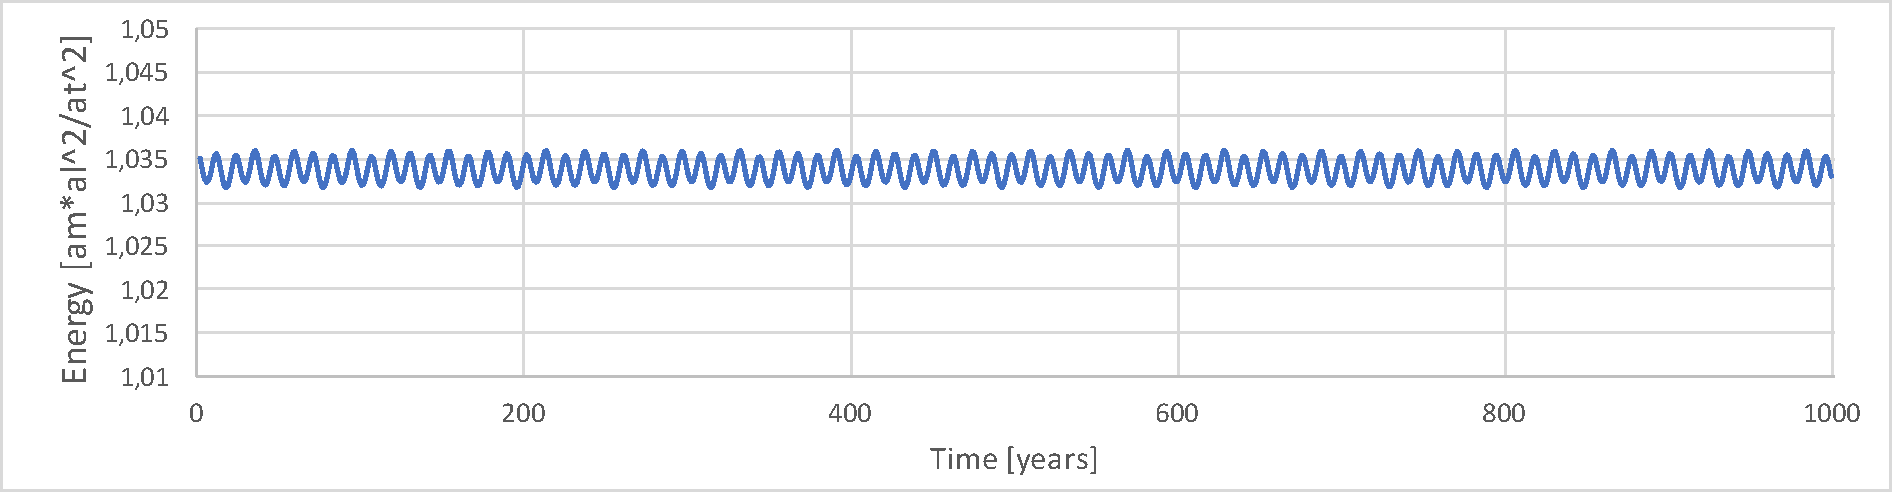
\includegraphics[scale=0.5]{solar_system_energy.pdf}
  \centering
  \caption{Sum of kinetic and potential energy of the Solar system. }
  \label{fig:solar_system_energy}
\end{figure}\vspace*{3pt}
Apart from the fluctuation, the total energy is preserved using the Velocity-Verlet integrator.


\subsection{Dam-break problem} \label{Dam-break_problem}
\subsubsection{Problem definition}
One of the most famous test cases of SPH is the two dimensional dam-break flow inside a rectangular, initially dry tank presented in Figure \ref{fig:dambreak_geom}.
\begin{figure}[H]
  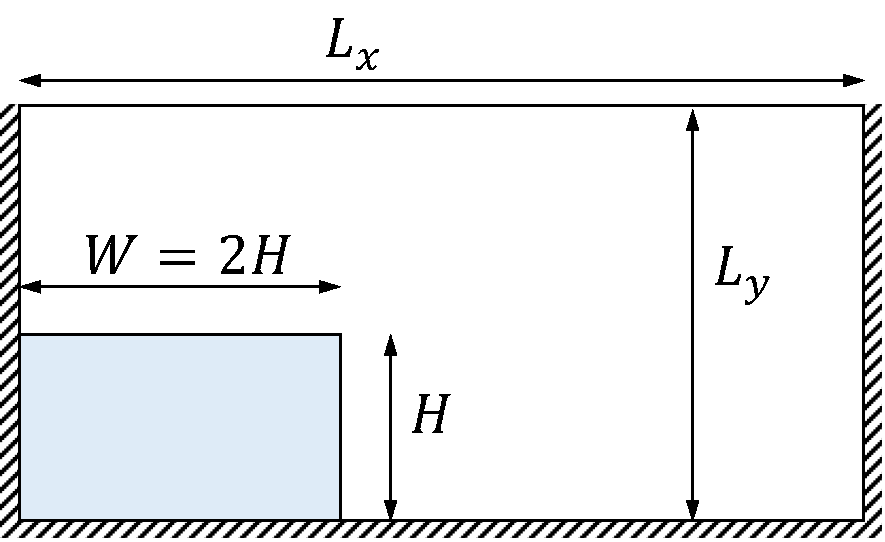
\includegraphics[scale=0.6]{dam_break_geom.pdf}
  \centering
  \caption{Initial configuration of the classical two-dimensional dam-break problem.}
  \label{fig:dambreak_geom}
\end{figure}\vspace*{3pt}

In Lagrangian frame the governing equations of the fluid can be written as
\begin{flalign} \label{eq:dam_break_pde}
\begin{split}
&\frac{d\rho}{dt}=-\rho\nabla \textbf{v}, \\
&\frac{d\textbf{v}}{dt}=-\frac{1}{\rho}\nabla p+\nu\Delta \textbf{v}, \\
\end{split}
\end{flalign}
where $p$ and $\rho$ are the pressure and density of the fluid, $\textbf{v}$ is the Lagrangian fluid velocity and $\nu$ is the physical kinematic viscosity of the fluid.
\subsubsection{Numerical model and results}
The discretized form of the equations \equref{eq:dam_break_pde} can be constructed similarly to the former SPH test cases:
\begin{flalign} \label{eq:dambreak_sph_discretized}
\begin{split}
&\frac{d\rho_i}{dt}=-\rho_i\sum{(\textbf{v}_j-\textbf{v}_i)\frac{m_j}{\rho_j}\nabla W_{ij}}+0.1ch\sum_j{2(\rho_j-\rho_i)\frac{\textbf{r}_{ij}}{|\textbf{r}_{ij}|^2}\frac{m_j}{\rho_j}\nabla W_{ij}}, \\
&\frac{d\textbf{v}_i}{dt}=-\sum_j{\bigg(\frac{p_i}{\rho_i^2}+\frac{p_j}{\rho_j^2}+Rf^n\bigg)m_j\nabla W_{ij}}+0.1ch\sum_j{\Pi_{ij}\frac{m_j}{\rho_j}\nabla W_{ij}}, \\
\end{split}
\end{flalign}
where $\sigma$ is the smoothing distance of the kernel function $W_{ij}$ and $\textbf{r}_{ij}=\textbf{r}_{i}-\textbf{r}_{j}$. The second term on the RHS of the equations \equref{eq:dambreak_sph_discretized} is the artificial density and velocity diffusion term respectively \cite{Antuono2012}. The application of the density diffusion term is often referred as the $\delta$-SPH formulation \cite{Molteni2009} and \cite{Antuono2010}. Since the equations \equref{eq:dambreak_sph_discretized} do not imply any constraint between the velocity and pressure fields, an additional state equation
\begin{equation} \label{eq:eos}
p_i=c^2(\rho-\rho_0),
\end{equation}
is required to couple the equations, where $\rho_0$ is the rest density of the fluid and $c$ is the speed of acoustic waves artificially reduced to ensure numerical stability beside reasonable time step size. Although exact incompressibility cannot be achieved using \equref{eq:eos}, the density variation can be limited to $\delta\rho=2\%$ by choosing $c=10\sqrt{gH}$.
Assuming the parameters of Table \ref{tbl:dam_break_params}, the following configuration file is required for Nauticle:
\begin{samepage}
\begin{example}{Dam break configuration file}{}
\lstset{basicstyle=\tiny}
\begin{lstlisting}[language=YAML]
simulation:
  case:
    workspace:
      constants:
        - Lx: 2
        - Ly: 1
        - H: 0.4
        - W: H*2
        - csize: Lx/100
        - dx: csize/2.1
        - h: csize/2
        - rho0: 1000
        - mass: dx^2*rho0
        - g: 0|-9.81
        - c: 10*sqrt(H*magnitude(g))
        - fluid: 0
        - wall: 1
        - CFL: 0.2
        - xi: 0.1
      variables:
        - dt: 0.0001
        - T: 0
      particle_system:
        domain:
          cell_size: csize|csize
          minimum: -Lx/2/csize-1|-Ly/2/csize-1
          maximum: Lx/2/csize+1|2*Ly/csize
          boundary: 0|0
        grid:
          gid: fluid
          gpos: -Lx/2|-Ly/2
          gsize: W|H
          goffset: 0|0
          gip_dist: dx|dx
        grid:
          gid: wall
          gpos: -Lx/2-csize|-Ly/2-csize
          gsize: csize|Ly+2*csize
          goffset: 0|0
          gip_dist: dx|dx
        grid:
          gid: wall
          gpos: -Lx/2|-Ly/2-csize
          gsize: Lx|csize
          goffset: 0|0
          gip_dist: dx|dx
        grid:
          gid: wall
          gpos: Lx/2|-Ly/2-csize
          gsize: csize|Ly+2*csize
          goffset: 0|0
          gip_dist: dx|dx
      fields:
        - a: 0|0
        - v: 0|0
        - rho: if(eq(gid,fluid),elem(g,1,0)*rho0*(elem(r,1,0)-H+Ly/2)/c^2+rho0,rho0)
        - rho_dot: 0
        - p: 0
    equations:
      - time: T=T+dt
      - cont: rho_dot=-rho*sph_D00(v,mass,rho,Wp52220,csize)
      - delta_sph: rho_dot=rho_dot+xi*c*h*sph_L0(rho,mass,rho,Wp52220,csize)
      - irho0: rho=euler(rho,rho_dot,dt)
      - EOS0: p=c^2*(rho-rho0)
      - acc0: a=-1/rho*(sph_G11(p,mass,rho,Wp32220,csize)+sph_T(dx,p,mass,rho,Wp32220,csize))+g
        condition: eq(gid,fluid)
      - acc1: a=a+xi*c*h*sph_A(v,mass,rho,Wp32220,csize)
        condition: eq(gid,fluid)
      - vel0: v=euler(v,a,dt)
        condition: eq(gid,fluid)
      - pos0: r=euler(r,v,dt)
        condition: eq(gid,fluid)
      - new_dt: dt=CFL*min(sqrt(h/fmax(magnitude(a))),h/c)
  parameter_space:
    simulated_time: 2
    print_interval: 0.02
    confirm_on_exit: 0
    output_format: ASCII
    compile_case: true
\end{lstlisting}
\end{example}
\end{samepage}
\begin{table} [H]
\begin{center}
\caption{Parameters of the dam-break simulation.}\label{tbl:dam_break_params}
\begin{tabular}{ l c r }
\toprule[1.5pt]
\bf Parameter & \bf Name & \bf Value \\
\midrule
Tank width & $L_x$ & $2$ m \\
Tank height & $L_y$ & $1$ m \\
Fluid initial height & $H$ & $0.4$ m \\
Fluid initial width & $W$ & $0.8$ m \\
\bottomrule[1.25pt]
\end{tabular}
\end{center}
\end{table}
Running the simulation of the collapse of the fluid column takes a while. Nevertheless, a few snapshots of the free surface shape is shown in Figure \ref{fig:dam_break_results}. 
\begin{figure}[H]
  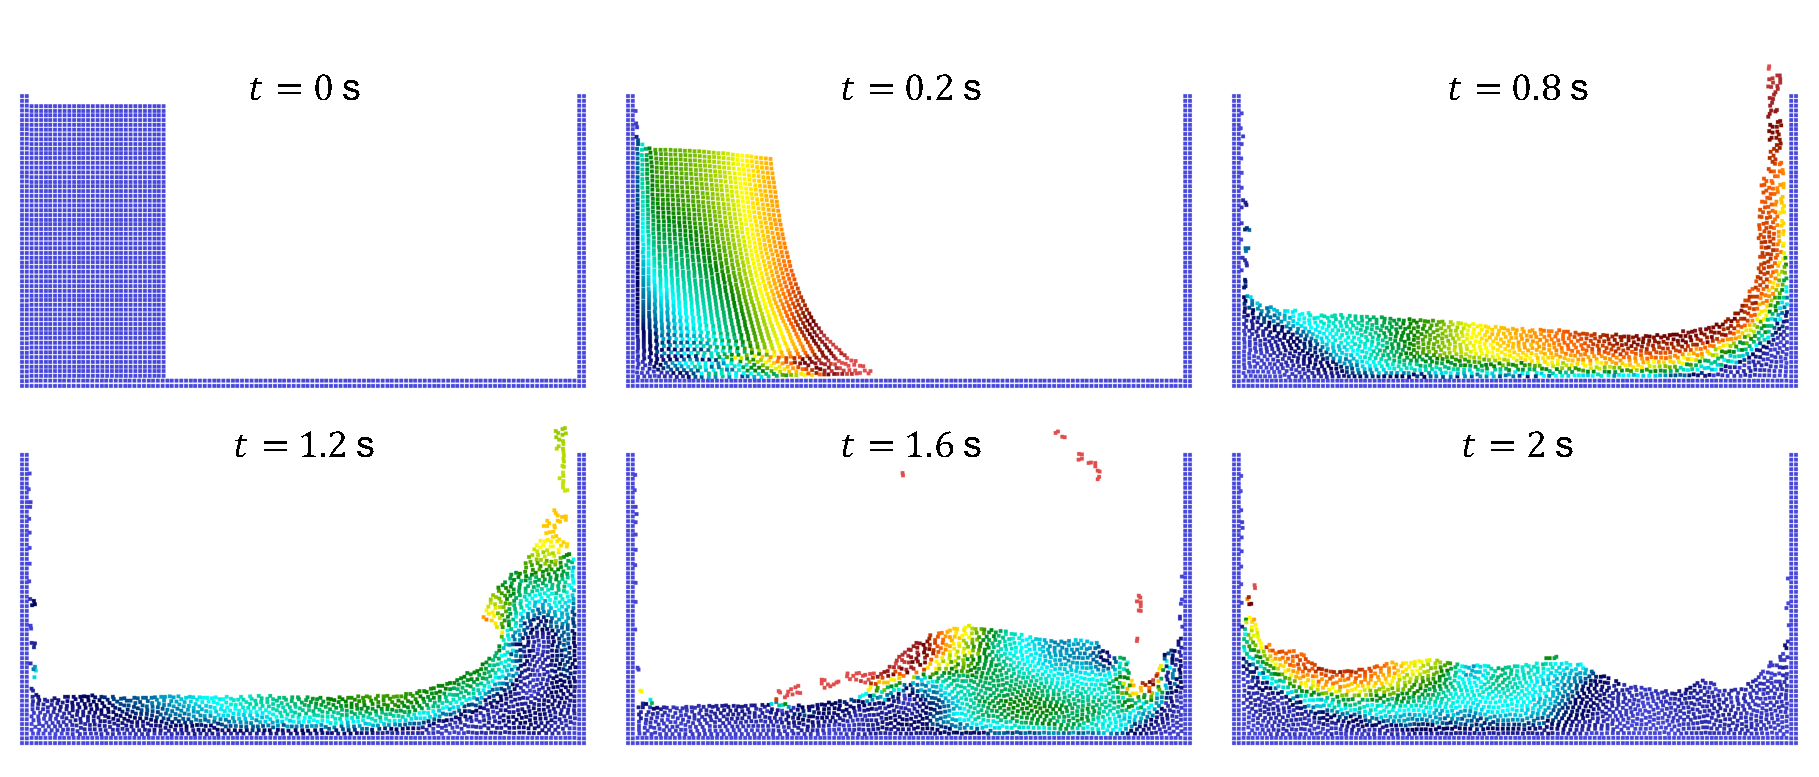
\includegraphics[scale=0.5]{dam_break_result.pdf}
  \centering
  \caption{Shape of the free surface in different time instants. Particles are colored by their velocities. }
  \label{fig:dam_break_results}
\end{figure}\vspace*{3pt}

\subsection{Dam-break problem with adaptive spatial resolution} \label{sec:SPH_adaptive}
Similarly to the former test case in section \ref{Dam-break_problem}, this example simulates a transient two-dimensional flow of a fluid body initially at rest. However, in the present section, the similar problem is modelled using an adaptive spatial resolution using the particle splitting and merging algorithm discussed in section \ref{splitting_merging}. Since the mathematical model is identical with the former example, the model definition is omitted here and merely the configuration file and the results are presented.
\begin{samepage}
\begin{example}{SPH dam-break with adaptive spatial resolution}{}
\lstset{basicstyle=\tiny}
\begin{lstlisting}[language=YAML]
simulation:
  case:
    workspace:
      constants:
        - Lx: 2
        - Ly: 1
        - H: 0.4
        - W: H*2
        - csize: Lx/100
        - dx: csize/2.1
        - rho0: 1000
        - g: 0|-9.81
        - c: 10*sqrt(H*magnitude(g))
        - fluid: 0
        - wall: 1
        - CFL: 0.2
        - bmin_x: 0.6
        - bmin_y: -Ly/2-csize
        - bmax_x: Lx/2+csize
        - bmax_y: -Ly/2+0.3
      variables:
        - dt: 0.0001
        - T: 0
      particle_system:
        domain:
          cell_size: csize|csize
          minimum: -Lx/2/csize-2|-Ly/2/csize-1
          maximum: Lx/2/csize+2|2*Ly/csize
          boundary: 0|0
        grid:
          gid: fluid
          gpos: -Lx/2|-Ly/2
          gsize: W|H
          goffset: 0|0
          gip_dist: dx|dx
        grid:
          gid: wall
          gpos: -Lx/2-csize|-Ly/2-csize
          gsize: csize|Ly+2*csize
          goffset: 0|0
          gip_dist: dx|dx
        grid:
          gid: wall
          gpos: -Lx/2|-Ly/2-csize
          gsize: Lx|csize
          goffset: 0|0
          gip_dist: dx|dx
        grid:
          gid: wall
          gpos: Lx/2|-Ly/2-csize
          gsize: csize|Ly+2*csize
          goffset: 0|0
          gip_dist: dx|dx
      fields:
        - norm: 0
        - mass: dx^2*rho0
        - h: csize/2
        - a: 0|0
        - v: 0|0
        - rho: if(eq(gid,fluid),elem(g,1,0)*rho0*(elem(r,1,0)-H+Ly/2)/c^2+rho0,rho0)
        - rho_dot: 0
        - p: 0
    equations:
      - normalization: norm=sph_S(1,mass,rho,Wp52220,2*h)
      # continuity equation
      - cont: rho_dot=-rho*sph_D00(v,mass,rho,Wp52220,2*h)/norm
      - delta_sph: rho_dot=rho_dot+0.5*c*h*sph_L0(rho,mass,rho,Wp52220,2*h)/norm
      - irho0: rho=euler(rho,rho_dot,dt)
      # equation of state
      - EOS0: p=c^2*(rho-rho0)
      # momentum equation
      - acc0: a=-1/rho*sph_G11(p,mass,rho,Wp52220,2*h)/norm+\
      0.1*c*h*sph_A(v,mass,rho,Wp52220,2*h)/norm+g
        condition: eq(gid,fluid)
      # integration and new time step
      - vel0: v=euler(v,a,dt)
        condition: eq(gid,fluid)
      - pos0: r=euler(r,v,dt)
        condition: eq(gid,fluid)
      - time: T=T+dt
      - new_dt: dt=CFL*min(sqrt(fmin(h/magnitude(a))),fmin(h)/c)
      - set_rho: rho=if(lt(rho,985),rho0,rho)
  parameter_space:
    simulated_time: 2
    print_interval: 0.01
    confirm_on_exit: 0
    output_format: ASCII
    file_start: 0
    compile_case: true
  splitter:
    condition: if(gt(elem(r,0,0),bmin_x)*lt(elem(r,0,0),bmax_x)*gt(elem(r,1,0),bmin_y)*\
    lt(elem(r,1,0),bmax_y),1,0)*eq(T,0)*eq(gid,wall)
    radius_field: h
    rotation: pi/4
    mass_field: mass
    smoothing_ratio: 1/sqrt(4)
    separation_parameter: 0.35
    daughters: 4
    parent: 0
    period: 1e10
  splitter:
    condition: if(gt(elem(r,0,0),bmin_x)*lt(elem(r,0,0),bmax_x)*gt(elem(r,1,0),bmin_y)*\
    lt(elem(r,1,0),bmax_y),1,0)*eq(gid,fluid)*gt(mass,dx^2*rho0/2)
    rotation: rand(-pi,pi)
    radius_field: h
    mass_field: mass
    smoothing_ratio: 1/sqrt(7)
    separation_parameter: 0.4
    daughters: 7
    parent: 1
    period: 1
  merger:
    condition: if(lt(elem(r,0,0),bmin_x-dx)+gt(elem(r,0,0),bmax_x+dx)+lt(elem(r,1,0),bmin_y-dx)+\
    gt(elem(r,1,0),bmax_y+dx),1,0)*neq(gid,wall)*lt(mass,dx^2*rho0*0.8)
    radius_field: h
    mass_field: mass
    velocity_field: v
    period: 1
    neighbor_condition: neq(gid,wall)
\end{lstlisting}
\end{example}
\end{samepage}
\begin{figure}[H]
  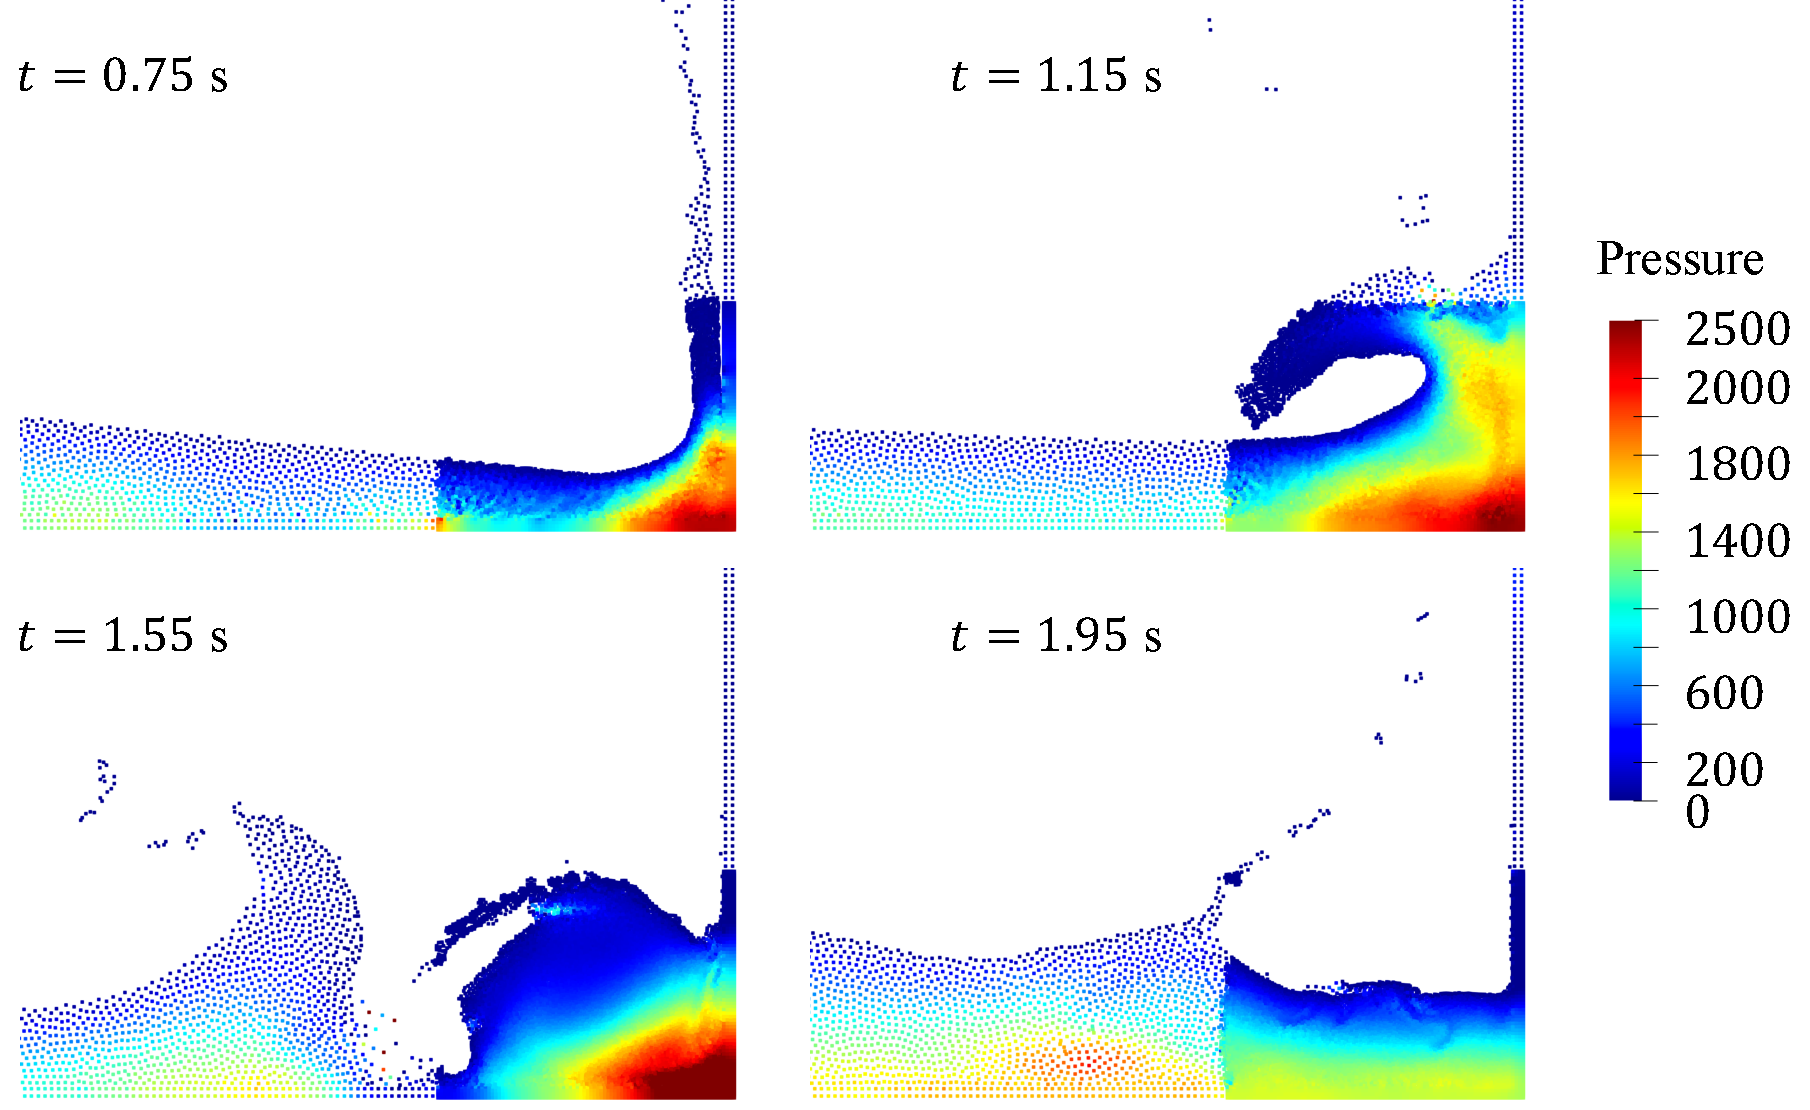
\includegraphics[scale=0.4]{adaptive_dam_break_results.pdf}
  \centering
  \caption{The lower right corner of the tank in different time instants.}
  \label{fig:stefan_problem_beam}
\end{figure}\vspace*{3pt}

\subsection{Stefan-problem}
\subsubsection{Problem definition}
Consider an $L=1$ m long one-dimensional solid beam of temperature $T_0=-0.2$ $^\circ$C with the melting temperature $T_m=0$ $^\circ$C. The ice is melted by the heat flux induced on one end by the constant temperature $T_w=0.1$ $^\circ$C. All the other sides of the beam are completely isolated from the environment. Figure \ref{fig:stefan_problem_beam} illustrates the phenomenon of the Stefan-problem.
\begin{figure}[H]
  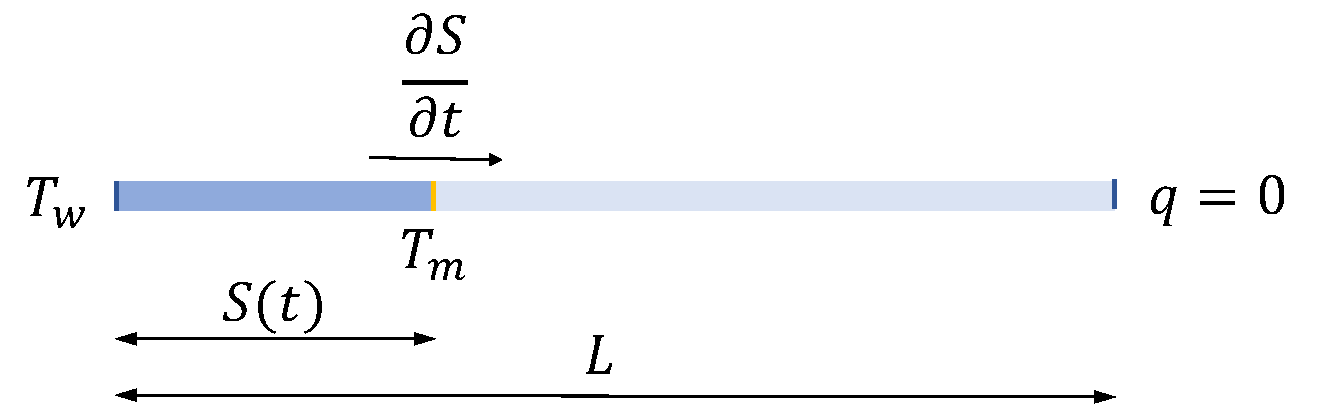
\includegraphics[scale=0.4]{stefan_problem_beam.pdf}
  \centering
  \caption{Melting solid beam heated on the left side. Darker and lighter shaded areas mark liquid and solid phases respectively. The yellow line referes to the interface with the melting temperature $T_m$.}
  \label{fig:stefan_problem_beam}
\end{figure}\vspace*{3pt}
The schematic layout of the temperatue distribution along the beam and the marching of the liquid-ice interface is determined by the equations below:
\begin{flalign} \label{eq:stefan_problem_heat}
&\frac{\partial T}{\partial t}=a\frac{\partial^2 T}{\partial x^2}, \\
&\frac{\partial S}{\partial t}=-\frac{\partial T}{\partial x}\bigg\vert_{S(t),t}.
\end{flalign} \label{eq:stefan_problem_interface}
Equation \equref{eq:stefan_problem_heat} is the one-dimensional heat equation and now describes the temperature diffusion in both the liquid and solid phases. The constant $a$ is the heat conduction coefficient with different values per each phase: $a_l=0.002$ m$^2/$s and $a_s=0.005$ m$^2/$s. The motion of the position $S(t)$ of the liquid-solid interface is proportional to the slope of the temperature, hence the heat flux at $S(t)$. By definition, the interface temperature is identical to the melting temperature, requiring the Dirichlet-condition to move together with the interface along the beam. Thus, the boundary conditions obtain the form of
\begin{flalign} \label{eq:stefan_problem_bc}
\begin{split}
& T(0,t)=0.1, \\
& T(S(t),t)=T_0, \\
& q=\firstpartial{T}{x}\bigg\vert_{x=L}=0
\end{split}
\end{flalign}
with the  the initial conditions
\begin{flalign} \label{eq:stefan_problem_ic}
\begin{split}
& T(x,0)=T_0=-0.2, \\
& S(0)=0.
\end{split}
\end{flalign}
\subsubsection{Numerical model and results}
To obtain the approximate solution in Nauticle, the discretized forms of \equref{eq:stefan_problem_heat} and \equref{eq:stefan_problem_interface} need to be constructed at first. Here, the SPH scheme is applied again to obtain
\begin{flalign} \label{eq:stefan_problem_sph}
\begin{split}
&\firstpartial{T}{t}=a_f\sum_j{\frac{2(T_j-T_i)}{|x_i-x_j|}\frac{m_j}{\rho_j}\firstpartial{W_{ij}}{x_j}}, \\
&\firstpartial{S}{t}=-\sum_j(T_j-T_i)\frac{m_j}{\rho_j}\firstpartial{W_{ij}}{x_j}.
\end{split}
\end{flalign}
The Dirichlet-conditions \equref{eq:stefan_problem_bc} are simply constrained in each time step as $S(t)$ changes. The configuration file to run the simulation of the Stefan-problem is as follows:
\begin{samepage}
\begin{example}{Stefan-problem configuration file}{}
\lstset{basicstyle=\tiny}
\begin{lstlisting}[language=YAML]
simulation:
  case:
    workspace:
      constants:
        - L: 1
        - csize: L/50
        - dx: csize/2.1
        - rho0: 1000
        - mass: dx*rho0
        - a_liquid: 0.002
        - a_solid: 0.005
        - wall: 0
        - liquid: 1
        - interface: 2
        - solid: 3
      variables:
        - Time: 0
        - dt: 0.01
        - S: dx*4
        - S_dot: 0
      particle_system:
        domain:
          cell_size: csize
          minimum: -1
          maximum: L/csize+1
          boundary: 0
        grid:
          gid: solid
          gpos: 0
          gsize: L
          goffset: 0
          gip_dist: dx
        grid:
          gid: wall
          gpos: -csize
          gsize: csize
          goffset: 0
          gip_dist: dx
      fields:
        - T: if(eq(gid,wall),0.2,-0.1)
        - T_dot: 0
        - x: elem(r,0,0)
    equations:
      - mb1: gid=interface
        condition: and(gt(x,S-dx/2),lt(x,S+dx/2))
      - mb2: gid=liquid
        condition: and(lt(x,S-dx/2-0.01),not(eq(gid,wall)))
      - mb3: gid=solid
        condition: gt(x,S+dx/2)
      - bc1: T=0
        condition: eq(gid,interface)
      - liquid: T_dot=a_liquid*sph_L0(T,mass,rho0,Wp22210,csize)
        condition: eq(gid,liquid)
      - solid: T_dot=a_solid*sph_L0(T,mass,rho0,Wp22210,csize)
        condition: eq(gid,solid)
      - i1: T=euler(T,T_dot,dt)
      - eq2: S_dot=fmax(if(eq(gid,interface),-sph_G00(if(neq(gid,solid),T,0),mass,rho0,Wp22210,csize),0))
      - i2: S=euler(S,S_dot,dt)
      - time: Time=Time+dt
  parameter_space:
    simulated_time: 40
    print_interval: 50*dt
    confirm_on_exit: 0
    output_format: ASCII
    compile_case: true
\end{lstlisting}
\end{example}
\end{samepage}
Please note that the temperature-dependency of the density is ignored during the simulation, furhtermore, the condition $q=0$ is satisfied naturally by the meshless SPH interpolant. As the result of the simulation the temperature distribution of the liquid and solid phases are plotted in Figure \ref{fig:stefan_problem_result}.
\begin{figure}[H]
  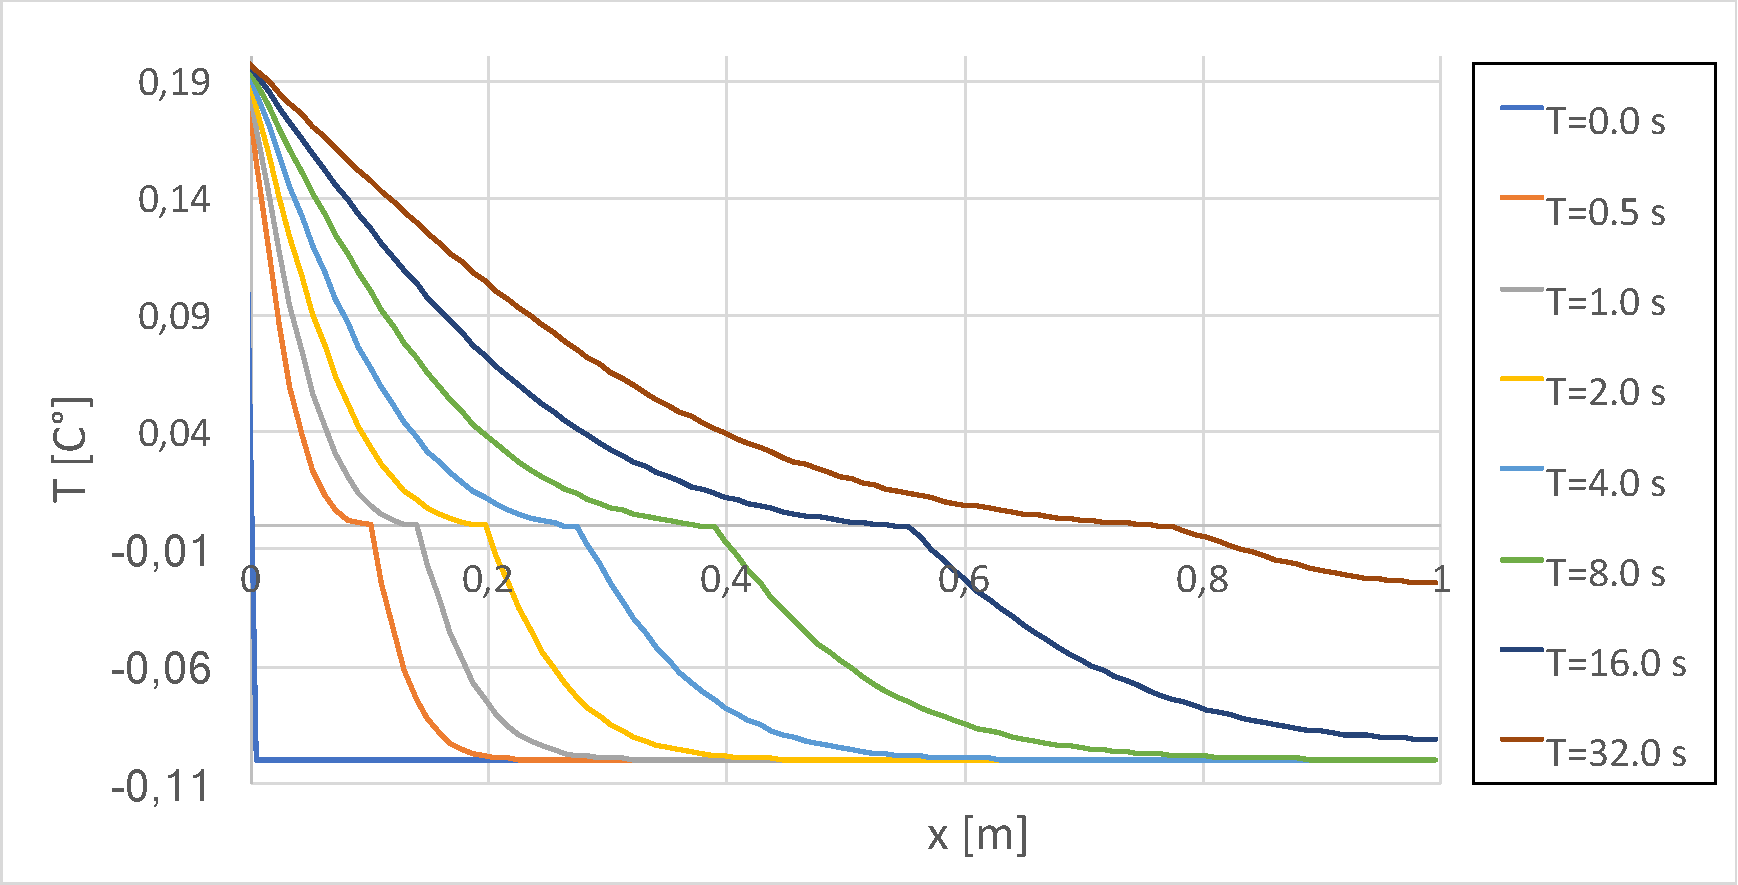
\includegraphics[scale=0.5]{stefan_problem_result.pdf}
  \centering
  \caption{Temperature distribution of the liquid and solid domains evaluated in different time instants.}
  \label{fig:stefan_problem_result}
\end{figure}\vspace*{3pt}

Finally, the propagation of the liquid-solid interface is displayed as a function of time in Figure \ref{fig:stefan_problem_result_s}.
\begin{figure}[H]
  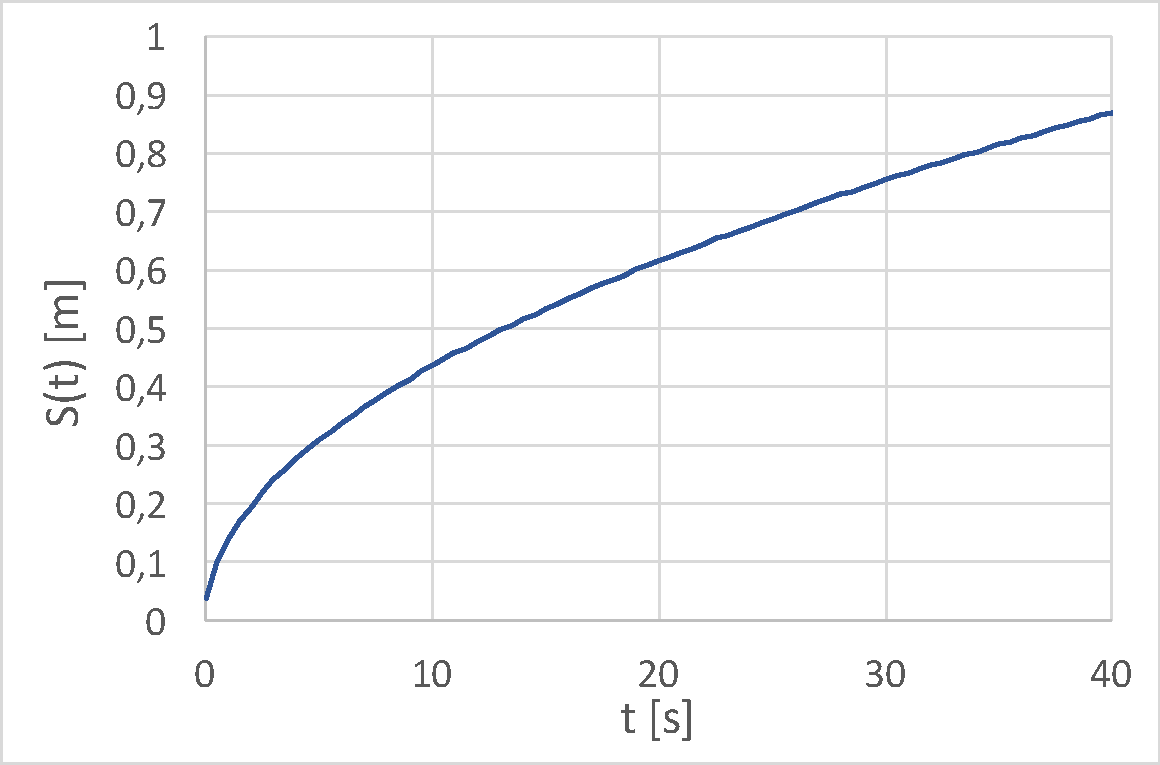
\includegraphics[scale=0.5]{stefan_problem_result_s.pdf}
  \centering
  \caption{Propagation of the liquid-solid interface $S(t)$.}
  \label{fig:stefan_problem_result_s}
\end{figure}\vspace*{3pt}


\subsection{Building evacuation} \label{sec:SFM_example}
\subsubsection{Problem definition}
Given a simplified single storey building with 7 rooms opening into the same corridor. Both exits occupy the same side of the building and open outwards. The sketch of the building is shown by Figure \ref{fig:building_sketch}.
\begin{figure}[H]
  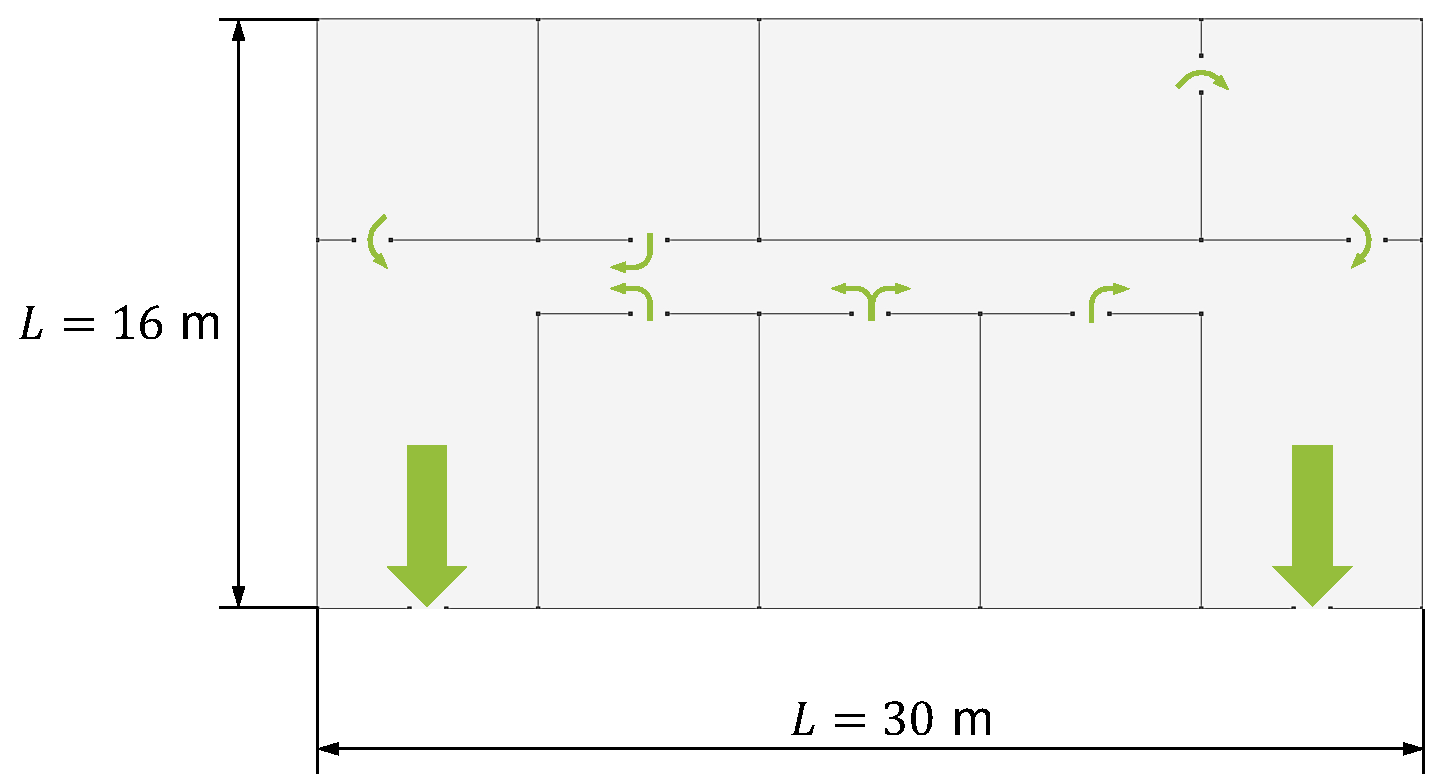
\includegraphics[scale=0.5]{building_sketch.pdf}
  \centering
  \caption{Sketch of the building to evacuate. Green arrows show the directions to leave the building.}
  \label{fig:building_sketch}
\end{figure}\vspace*{3pt}
It is assumed that 120 initially randomly distributed people aim to leave the building in the shortest possible direction.
\subsubsection{Numerical model and results}
Again, the governing equation of the standard SFM:
\begin{flalign}
&\frac{d\textbf{v}_i}{dt}=\frac{v_0\textbf{e}_0-\textbf{v}_i}{\tau}-\frac{1}{m_i}\sum_{j\neq i}{\bigg[A_i exp\bigg(\frac{R_{ij}-d_{ij}}{B_i}\bigg)+k(R_{ij}-d_{ij})-c_{ij}\bigg]\textbf{n}_{ji}},
\end{flalign}
which can be solved by numerical integration, accordingly, the explicit Euler scheme has been chosen. The constants $A$, $B$, $k$, $c$ are considered to be identical for each individual person. The desired position of each person is calculated based on the current position, hence it is automatically updated as a person leaves a room.
The mass of the individuals is randomly distributed between $50$ kg and $100$ kg and used to calculate the sizes with the linear function
\begin{flalign}
R_i=0.002m_i+0.15.
\end{flalign}
The desired velocities are also randomly chosen independently from the sizes. To prevent people from crossing any of the walls, the boundary conditions (hence the building) is built up using nodes having the same properties as the people except that they are fixed in space during the whole simulation. The discretized building is shown by Figure \ref{fig:discretized_building}. The $R_w$ radii of the wall-nodes are constant and $R_w=0.1$ m. 
\begin{figure}[H]
  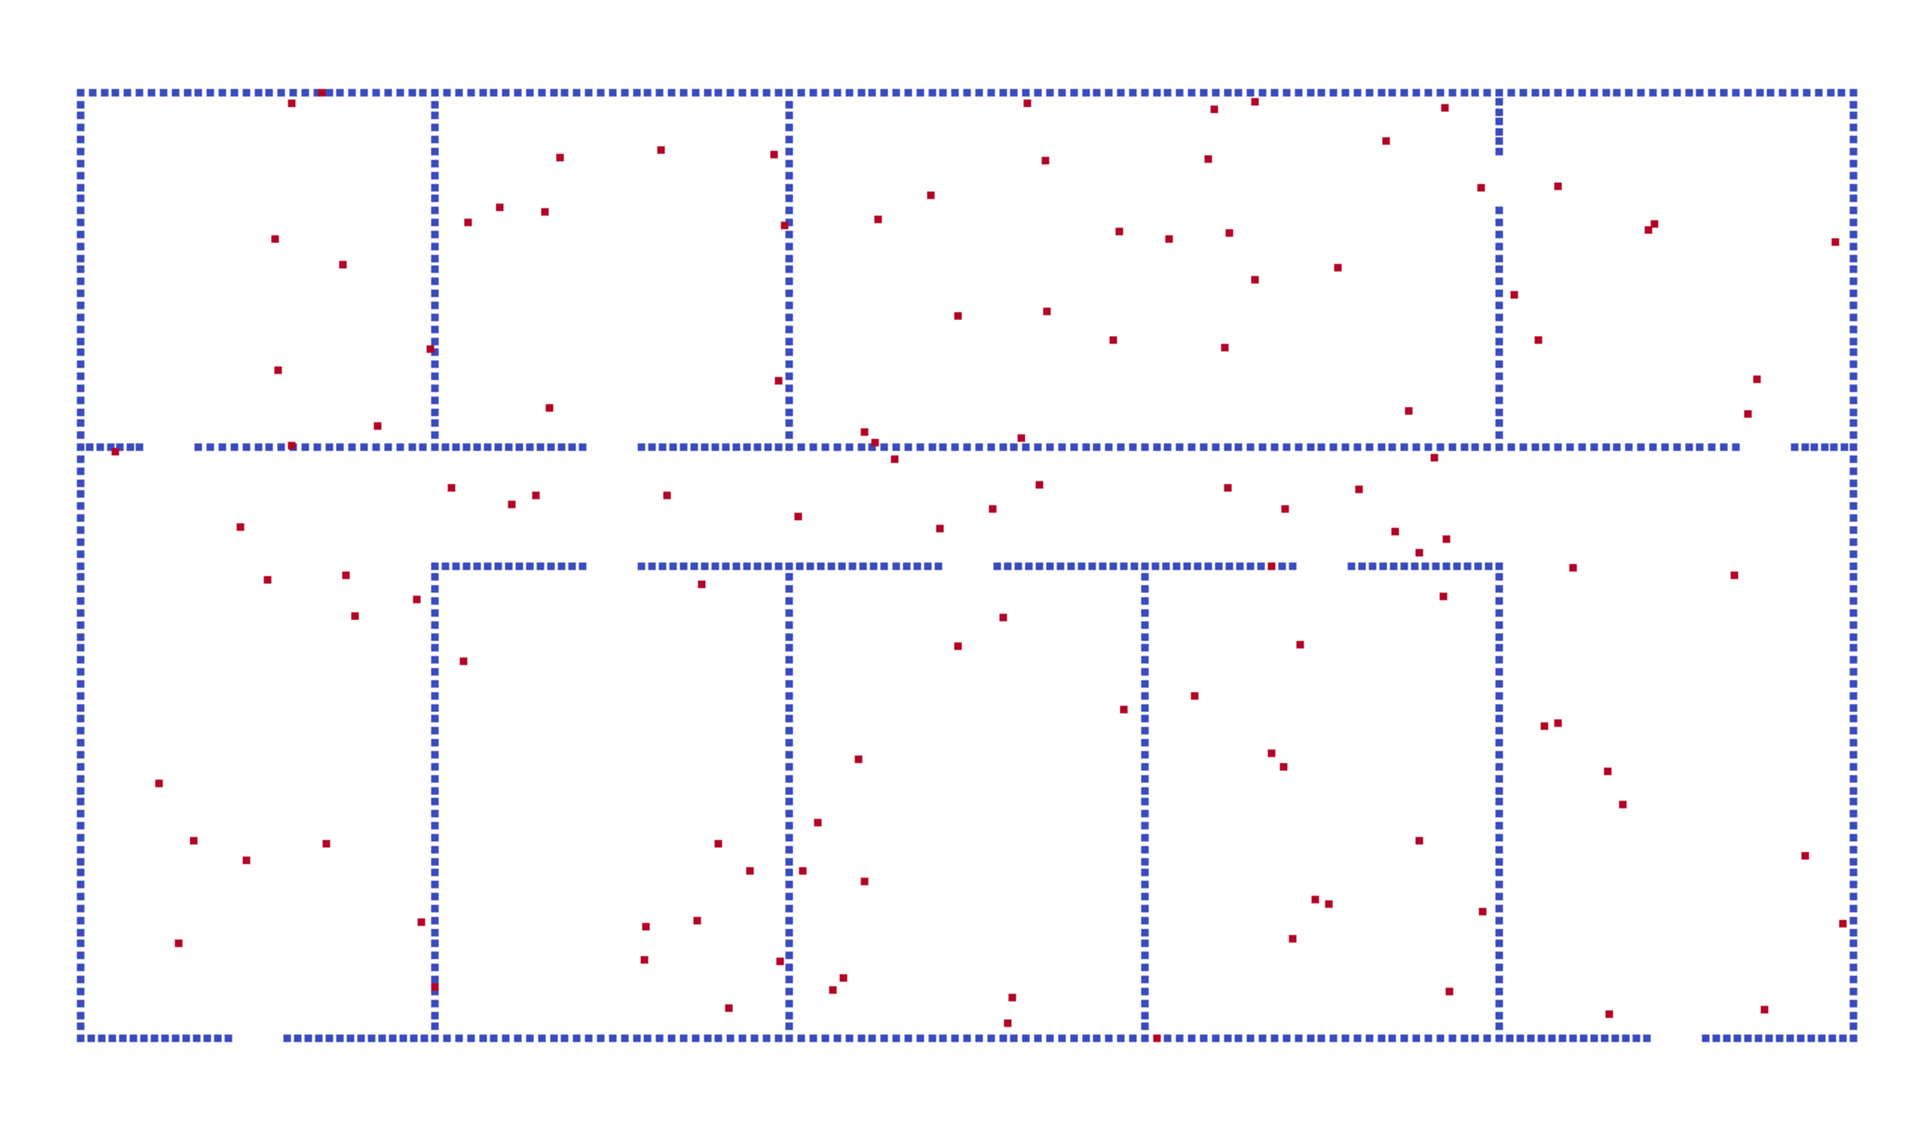
\includegraphics[scale=0.25]{discretized_building.pdf}
  \centering
  \caption{Discretization of the building by fixed nodes (blue) and initial distribution of people (red). }
  \label{fig:discretized_building}
\end{figure}\vspace*{3pt}
Altough the initial condition seems to be unphysical due to the interference of people and wall nodes, the repulsion model rapidly forces red nodes to a feasible position without significantly influencing the results.
Running the following configuration file
\begin{samepage}
\begin{example}{Evacuation configuration file}{}
\lstset{basicstyle=\tiny}
\begin{lstlisting}[language=YAML]
simulation:
  case:
    workspace:
      constants:
        - L: 40
        - c_s: 1
        - dx: 1
        - k: 1000
        - d1: -13.5|10
        - d2: -6|10
        - d3: 9|14.5
        - d4: 13.5|10
        - d5: -6|8
        - d6: 0|8
        - d7: 6|8
        - d8: -9|9
        - d9: 9|9
        - d10: -12|0
        - d11: 12|0
        - d12: 0|-10
        - R_w: 0.1
      variables:
        - T: 0
        - dt: 0.01
      particle_system:
        domain:
          cell_size: c_s|c_s
          minimum: -L/c_s|-L/c_s
          maximum: L/c_s|L/c_s
          boundary: periodic|periodic
        grid:
          gid: 2
          file: walls.xyz
        grid:
          gid: 1
          file: people.xyz
      fields:
        - A: 10
        - B: 0.2
        - c: 0.1
        - m: rand(50,100)
        - p0: 0|0
        - v0: if(eq(gid,1),rand(2,4),0)
        - tau: 2
        - R: if(eq(gid,2),R_w,0.002*m+0.15)
        - a: 0|0
        - v: 0|0
        - x: elem(r,0,0)
        - y: elem(r,1,0)
    equations:
      - time: T=T+dt
      - pos_x: x=elem(r,0,0)
        condition: eq(gid,1)
      - pos_y: y=elem(r,1,0)
        condition: eq(gid,1)
      - wp_1: p0=if(and(lt(x,-9),gt(y,10)),d1,p0)
        condition: eq(gid,1)
      - wp_2: p0=if(and(and(gt(x,-9),lt(x,-3)),gt(y,10)),d2,p0)
        condition: eq(gid,1)
      - wp_3: p0=if(and(and(gt(x,-3),lt(x,9)),gt(y,10)),d3,p0)
        condition: eq(gid,1)
      - wp_4: p0=if(and(gt(x,9),gt(y,10)),d4,p0)
        condition: eq(gid,1)
      - wp_5: p0=if(and(and(gt(x,-9),lt(x,-3)),lt(y,8)),d5,p0)
        condition: eq(gid,1)
      - wp_6: p0=if(and(and(gt(x,-3),lt(x,3)),lt(y,8)),d6,p0)
        condition: eq(gid,1)
      - wp_7: p0=if(and(and(gt(x,3),lt(x,9)),lt(y,8)),d7,p0)
        condition: eq(gid,1)
      - wp_8: p0=if(and(and(gt(x,-9),lt(x,0)),and(gt(y,8),lt(y,10))),d8,p0)
        condition: eq(gid,1)
      - wp_9: p0=if(and(and(gt(x,0),lt(x,9)),and(gt(y,8),lt(y,10))),d9,p0)
        condition: eq(gid,1)
      - wp_10: p0=if(and(lt(x,-9),lt(y,10)),d10,p0)
        condition: eq(gid,1)
      - wp_11: p0=if(and(gt(x,9),lt(y,10)),d11,p0)
        condition: eq(gid,1)
      - wp_12: p0=if(lt(y,0),d12,p0)
        condition: eq(gid,1)
      - acceleration: v=sfm(v,p0,v0,m,R,A,B,k,c,tau)
        condition: eq(gid,1)
      - velocity: v=euler(v,a,dt)
        condition: eq(gid,1)
      - position: r=euler(r,v,dt)
        condition: eq(gid,1)
  parameter_space:
    simulated_time: 60
    print_interval: 0.1
    confirm_on_exit: 0
    file_start: 0
    output_format: ASCII
    compile_case: true
\end{lstlisting}
\end{example}
\end{samepage}
in Nauticle performs the simulation of the evacuation of the building for one minute of simulation time. The snapshots of the process in different time instants are shown by Figure \ref{fig:SMF_result}.
\begin{figure}[H]
  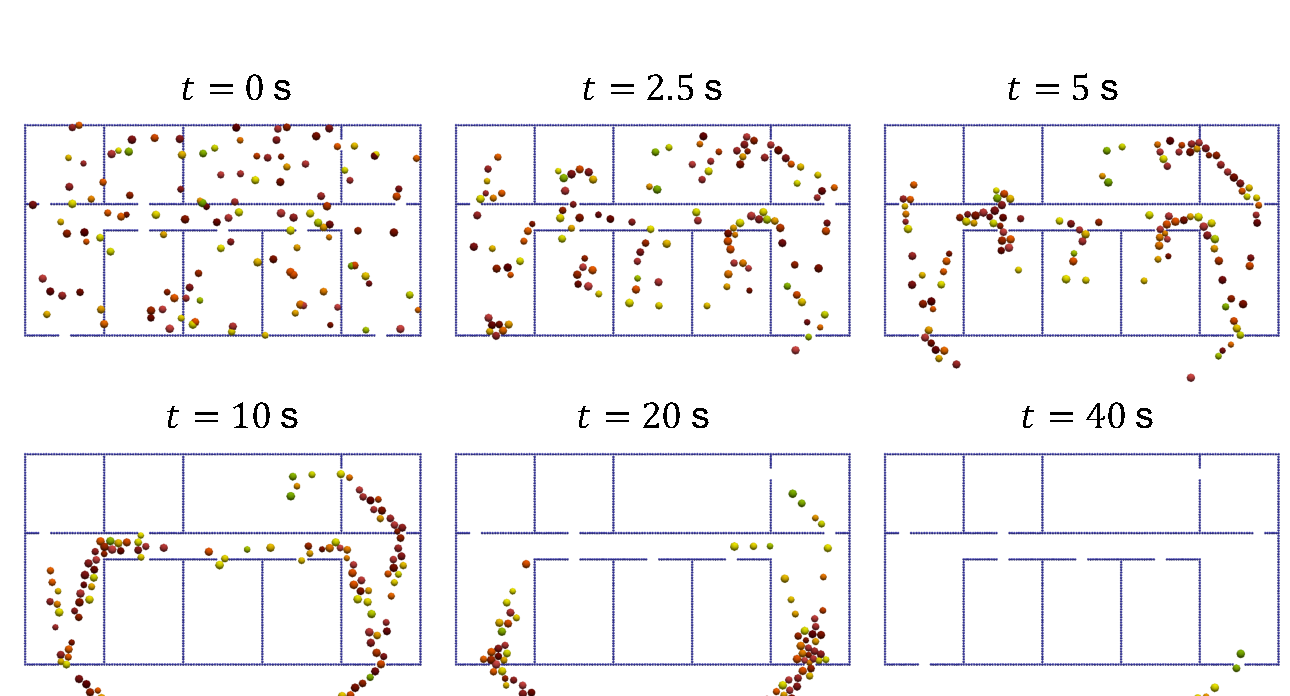
\includegraphics[scale=0.6]{evacuation_result.pdf}
  \centering
  \caption{Evacuation process based on the SFM-model. The size of the nodes are equal to their radii and colored by the associated desired velocities.}
  \label{fig:SMF_result}
\end{figure}\vspace*{3pt}
The complete evacuation occured in slightly more than $40$ seconds.

\subsection{Molecular dynamics simulation} \label{sec:MD_example}
\subsubsection{Problem definition}
Consider a two-dimensional square-shaped domain with edge size $L=20$ m, in which a set of particles aligned initially over a uniform lattice shown in Figure \ref{fig:MD_ic}.
\begin{figure}[H]
  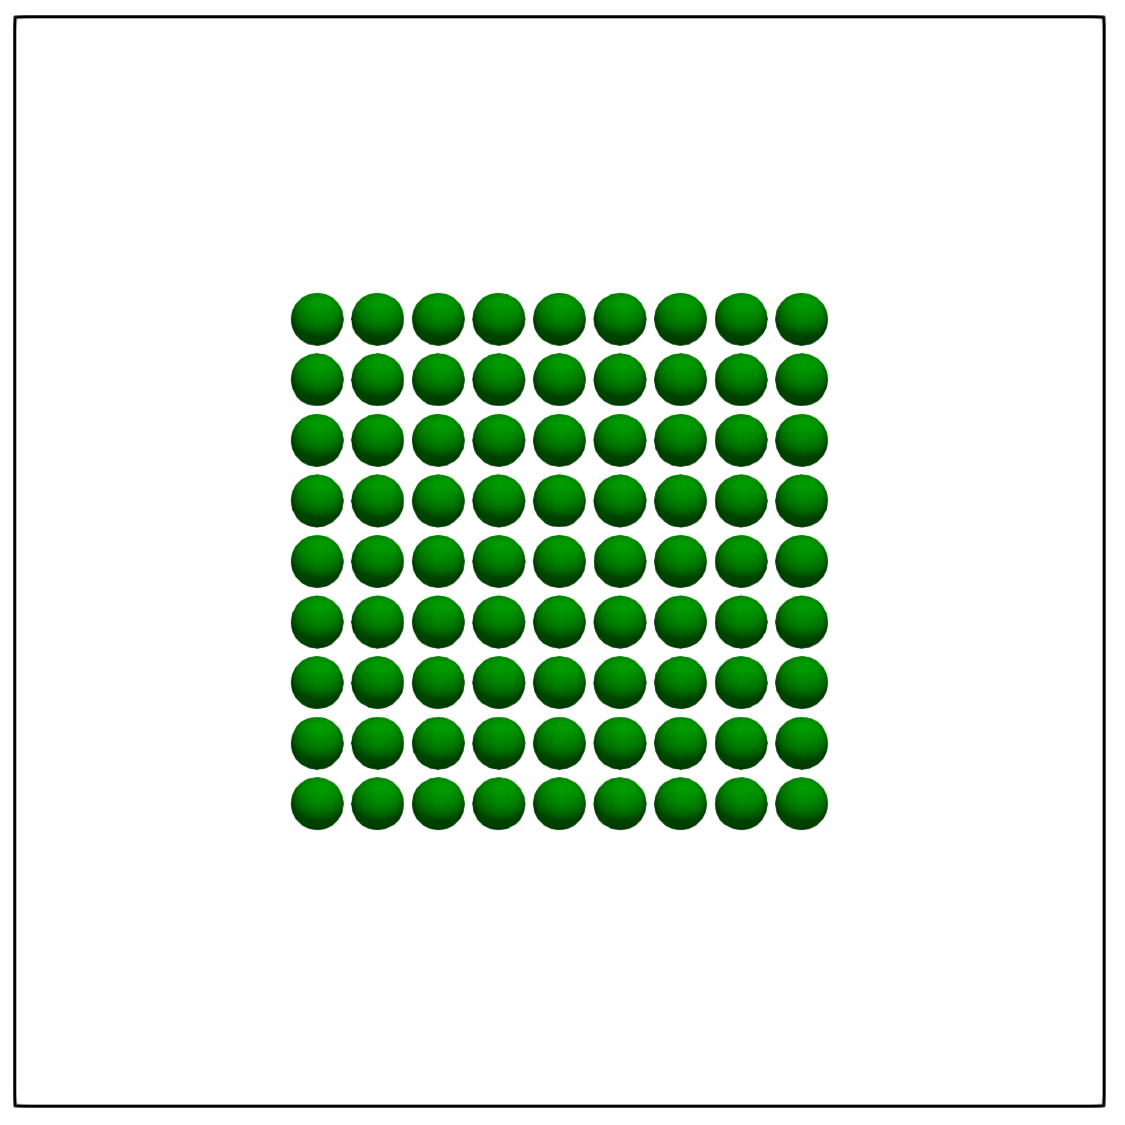
\includegraphics[scale=0.3]{md_ic.pdf}
  \centering
  \caption{Initial condition of the particle layout in the square domain.}
  \label{fig:MD_ic}
\end{figure}\vspace*{3pt}
The particle mass the radii $\sigma$ and the interaction magnitudes $\epsilon$ are considered to be one, and $r_{cut}=3$ m. According to the Lennard-Jones potential, the system of particles can be written as:
\begin{flalign}
\frac{dv_i}{dt}=-\sum_{j\neq i}{\frac{48\epsilon}{\vert\textbf{r}_{ji}\vert^2}\bigg(\bigg(\frac{\sigma}{\vert\textbf{r}_{ji}\vert}\bigg)^{12}-\frac{1}{2}\bigg(\frac{\sigma}{\vert\textbf{r}_{ji}\vert}\bigg)^6\bigg)\textbf{r}_{ji}},
\end{flalign}
which is in this case intergrated numerically using the velocity-Verlet scheme. The simple mathematical model can be built using the $md(\epsilon,\sigma,r_{cut})$ operator, hence the configuration file obtians the following form:
\begin{samepage}
\begin{example}{Lennard-Jones configuration file}{}
\lstset{basicstyle=\tiny}
\begin{lstlisting}[language=YAML]
simulation:
  case:
    workspace:
      constants:
        - Lx: 20
        - cell_size: 4
      variables:
        - dt: 0.01
      particle_system:
        domain:
          cell_size: cell_size|cell_size
          minimum: 0|0
          maximum: Lx/cell_size|Lx/cell_size
          boundary: symmetric|symmetric
        grid:
          gid: 0
          gpos: 5|5
          gsize: 10|10
          goffset: 0|0
          gip_dist: 1.1|1.1
      fields:
        - v: rand(-0.1,0.1)|rand(-0.1,0.1)
        - a: 0|0
    equations:
      - pos: r=verlet_r(r,v,a,dt)
      - acceleration: a=md(1,1,3)
      - vel: v=verlet_v(v,a,dt)
  parameter_space:
    simulated_time: 10
    print_interval: 0.1
    compile_case: true
\end{lstlisting}
\end{example}
\end{samepage}
As it can be seen, the initial velocity of the particles were chosen randomly in both $x$ and $y$ directions within the range $[-0.1,0.1]$. Finally, the particle positions after $10$ s is presented in Figure \ref{fig:MD_results}.
\begin{figure}[H]
  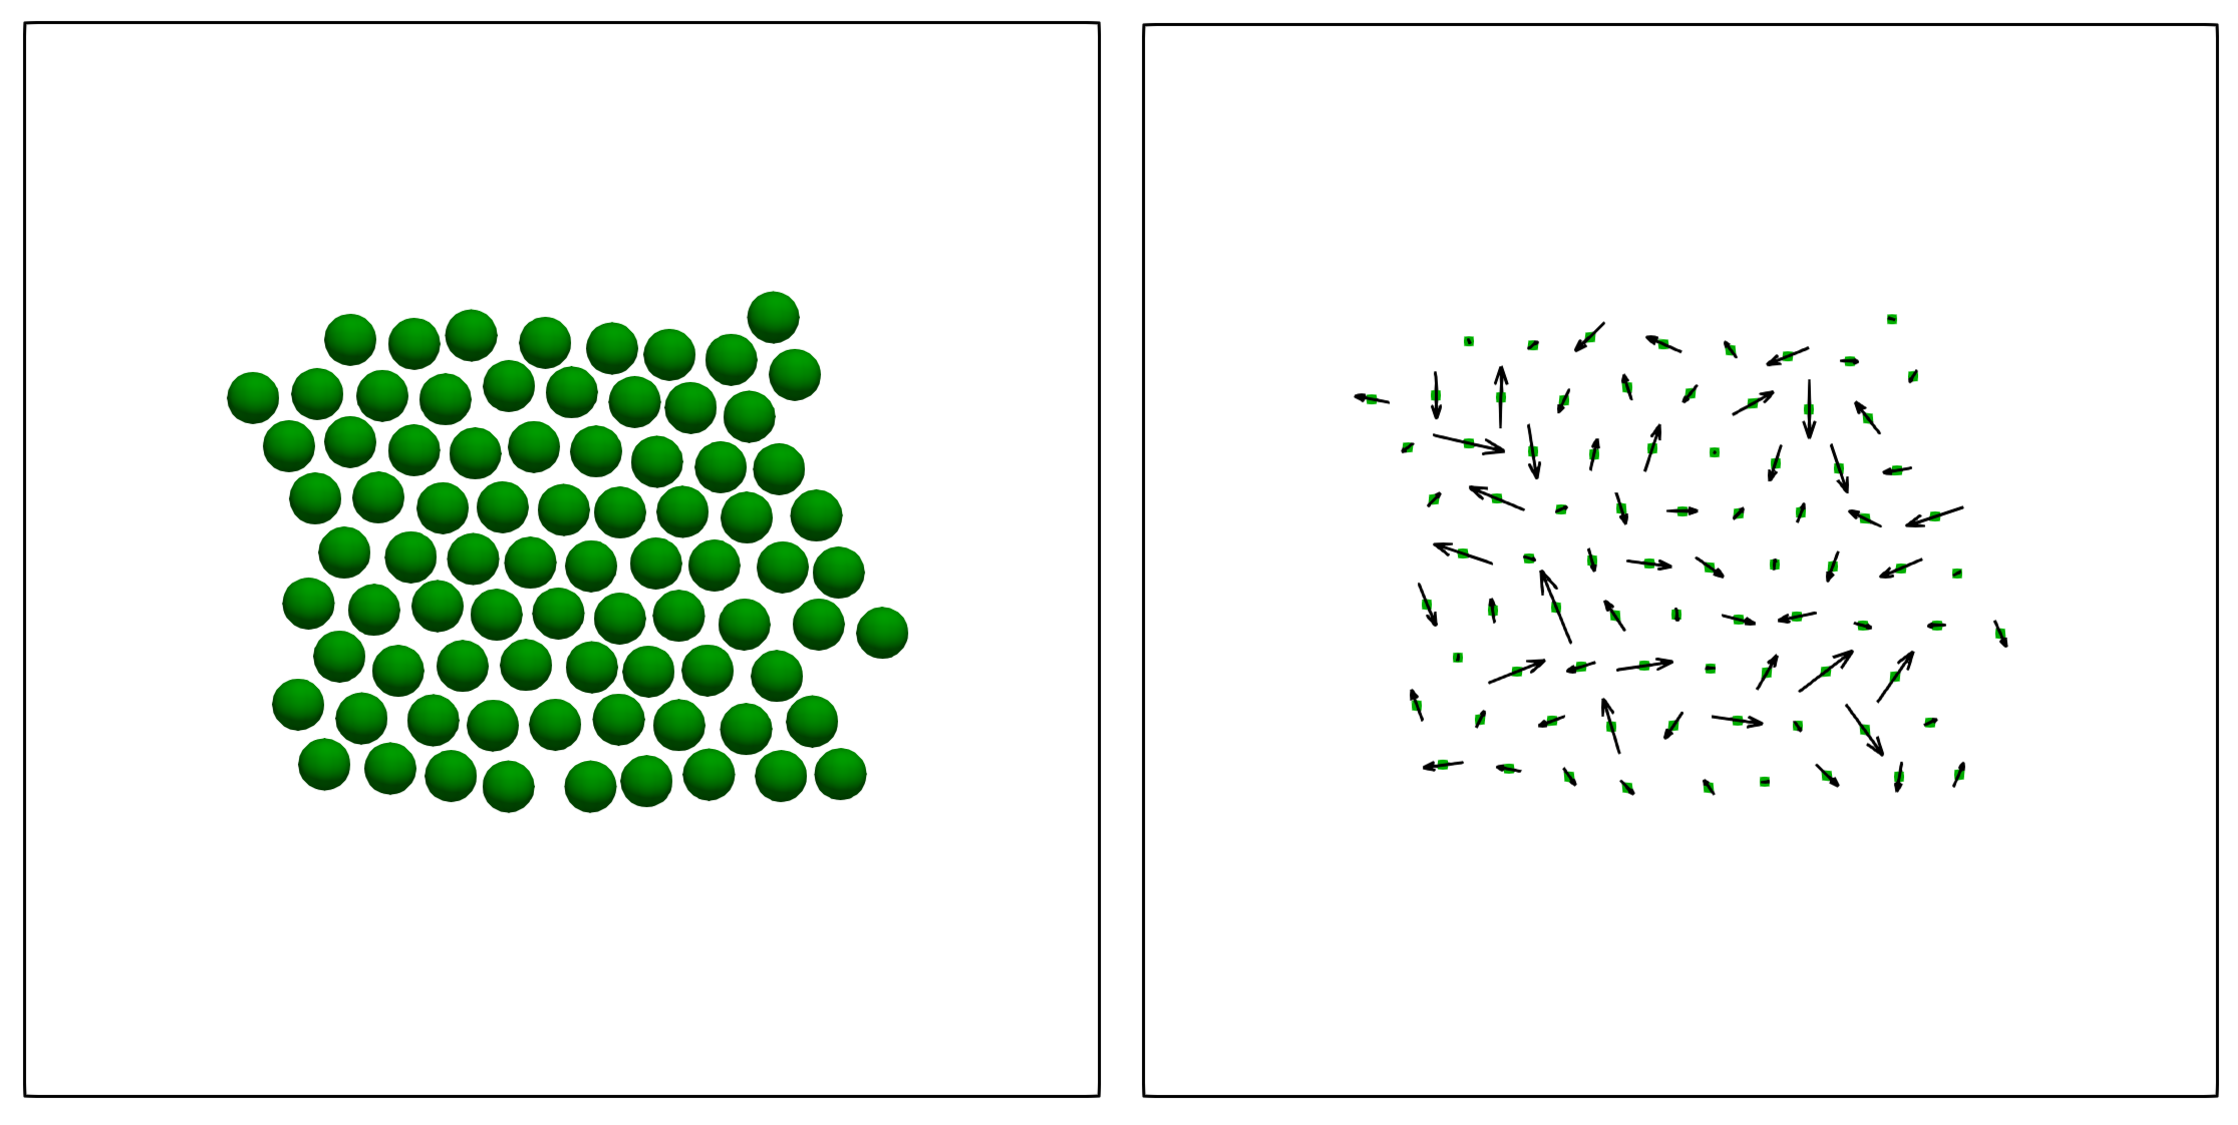
\includegraphics[scale=0.3]{md_results.pdf}
  \centering
  \caption{Particle positions (left) and velocities (right) at the time instant $t=10$ s.}
  \label{fig:MD_results}
\end{figure}\vspace*{3pt}
Since there is no dissipation in the simulation, the particles do not occupy stationary equilibrium states.

\section{The Nauticle open-source code}
This section comments the role of each source and header file of Nauticle. For better clarity, the explanation is divided into different groups marked by the subsequent sections.
\subsection{Nodes of the expression tree}

\textbf{pmExpression.h / pmExpression.cpp} \\
Declares / defines the main node in the expression tree (abstract class).

\textbf{pmSymbol.h / pmSymbol.cpp} \\
Declares / defines the symbol node in the expression tree (abstract class).

\textbf{pmSingle.h / pmSingle.cpp} \\
Declares / defines the single node in the expression tree (abstract class).

\textbf{pmConstant.h / pmConstant.cpp} \\
Declares / defines the constant node in the expression tree.

\textbf{pmVariable.h / pmVariable.cpp} \\
Declares / defines the variable node in the expression tree.

\textbf{pmField.h / pmField.cpp} \\
Declares / defines the field node in the expression tree.

\textbf{pmParticle\_system.h / pmParticle\_system.cpp} \\
Declares / defines the particle system node in the expression tree.

\textbf{pmOperator.h} \\
Declares / defines the operator node in the expression tree (abstract class).

\textbf{pmArithmetic\_function.h} \\
Declares / defines the class of arithmetic functions in the expression tree.

\textbf{pmArithmetic\_operator.h} \\
Declares / defines the class of arithmetic operators in the expression tree.


\subsubsection{Nodes of the interaction branch}

\textbf{pmInteraction.h} \\
Declares / defines the interaction node in the expression tree (abstract class).

\textbf{pmNeighbors.h / pmNeighbors.cpp} \\
Declares / defines the neighbor interaction node in the expression tree.

\textbf{pmNbody\_operator.h / pmNbody\_operator.cpp} \\
Declares / defines the gravitational interaction in the expression tree.

\textbf{pmDem\_operator.h} \\
Declares / defines the Discrete Element Method interaction in the expression tree.

\textbf{pmFilter.h} \\
Declares / defines the filter node in the expression (tree abstract class).

\textbf{pmDvm\_operator.h / pmDvm\_operator.cpp} \\
Declares / defines the Discrete Vortex Method interaction in the expression tree.

\textbf{pmSph\_operator.h} \\
Declares / defines the Smoothed Particle Hydrodynamics interaction in the expression tree.

\textbf{pmSfm\_operator.h / pmSfm\_operator.cpp} \\
Declares / defines the Social Force Model interaction in the expression tree.

\textbf{pmMd\_operator.h / pmMd\_operator.cpp} \\
Declares / defines the Molecular dynamics interaction in the expression tree.

\textbf{pmFmax.h / pmFmax.cpp} \\
Declares / defines the class that calculates the maximum of the given field.

\textbf{pmFmean.h / pmFmean.cpp} \\
Declares / defines the class that calculates the mean of the given field.

\textbf{pmFmin.h / pmFmin.cpp} \\
Declares / defines the class that calculates the minimum of the given field.

\textbf{pmFsearch.h / pmFsearch.cpp} \\
Declares / defines the class from which the minimum, maximum, mean, and sum interactions are inherited (abstract class).

\textbf{pmFsum.h / pmFsum.cpp} \\
Declares / defines the class that calculates the sum of the given field.

\textbf{pmKuramoto\_operator.h / pmKuramoto\_operator.cpp} \\
Declares / defines the class that calculates the Kuramoto synchronizer term of the given field.


\subsection{Input/Output files}

\textbf{pmVTK\_manager.h / pmVTK\_manager.cpp} \\
Declares / defines the parent class of VTK read and write classes (abstract class).

\textbf{pmVTK\_reader.h / pmVTK\_reader.cpp} \\
Declares / definesthe class for reading initial conditions from VTK files.

\textbf{pmVTK\_writer.h / pmVTK\_writer.cpp} \\
Declares / defines class for writing results to VTK files.

\textbf{pmYAML\_processor.h / pmYAML\_processor.cpp} \\
Declares / defines the class that reads the configuration file and generates the simulation case based on it.

\textbf{pmLog\_stream.h / pmLog\_stream.cpp} \\
Declares / defines the class for writing functions.


\subsection{Files of simulation case}

\textbf{pmBackground.h / pmBackground.cpp} \\
Declares / defines the class representing a field represented over an unstructured grid.

\textbf{pmCase.h / pmCase.cpp} \\
Declares / defines the case class representing simulation case.

\textbf{pmSimulation.h / pmSimulation.cpp} \\
Declares / defines the class for simulation management like solution of equations and writing results.

\textbf{pmCommand\_parser.h / pmCommand\_parser.cpp} \\
Declares / defines the class to parse runtime commands.

\textbf{pmDomain.h / pmDomain.cpp} \\
Declares / defines the class holding information about the simulation domain and its boundaries.

\textbf{pmEquation.h / pmEquation.cpp} \\
Declares / defines the class that holds a single user-defined equation.

\textbf{pmEquation\_parser.h / pmEquation\_parser.cpp} \\
Declares / defines the class of user-defined equation parsing.

\textbf{pmExpression\_parser.h / pmExpression\_parser.cpp} \\
Declares / defines the class to parse user-defined expressions.

\textbf{pmGrid.h / pmGrid.cpp} \\
Declares / defines the class that generates one-, two- or three-dimensional grids.

\textbf{pmGrid\_space.h / pmGrid\_space.cpp} \\
Declares / defines the class that stores the grids specified during the simulation.

\textbf{pmKernel\_includes.h / pmKernel\_includes.cpp} \\
Collects the implemented kernel functions for inclusion.

\textbf{pmKernel\_function.h / pmKernel\_function.cpp} \\
Declares / defines the base class of kernel functions.

\textbf{pmKernel.h / pmKernel.cpp} \\
Declares / defines the class for wrapping kernel functions.

\textbf{pmZeroth\_order\_kernel.h} \\
Declares / defines the class that implements the zeroth order kernel function.

\textbf{pmFirst\_order\_kernel.h} \\
Declares / defines the class that implements the first order kernel function.

\textbf{pmSecond\_order\_kernel.h} \\
Declares / defines the class that implements the second order kernel function.

\textbf{pmThird\_order\_kernel.h} \\
Declares / defines the class that implements the third order kernel function.

\textbf{pmFifth\_order\_kernel.h} \\
Declares / defines the class that implements the fifth order kernel function.

\textbf{pmGaussian\_kernel.h} \\
Declares / defines the class that implements the gaussian kernel function.

\textbf{pmMath\_parser.h / pmMath\_parser.cpp} \\
Declares / defines the class with math parsing methods (abstract class).

\textbf{pmMath\_test.h / pmMath\_test.cpp} \\
Declares / defines the class that checks if a name in the user-defined equation is a function name.

\textbf{pmNoncopyable.h} \\
Declares / defines the class that prevents to copy any of the object of its derived classes (abstract class).

\textbf{pmParameter\_space.h / pmParameter\_space.cpp} \\
Declares / defines the class that stores the parameters of the simulation.

\textbf{pmRandom.h / pmRandom.cpp} \\
Declares / defines functions for random number generation.

\textbf{pmSort.h} \\
Declares / defines the function to sort data.

\textbf{pmTensor.h / pmTensor.cpp} \\
Declares / defines the fundamental quantity tensor in the expression tree.

\textbf{pmTensor\_parser.h / pmTensor\_parser.cpp} \\
Declares / defines the class that performs the parsing of user-defined expressions.

\textbf{pmWorkspace.h / pmWorkspace.cpp} \\
Declares / defines the class for the workspace that keeps the simulation data defined by the user.

\subsubsection{Files of the precompilation and dynamic linking.}

\textbf{pmInterface.h} \\
Declares / defines the interface class for the dynamically linking.

\textbf{pmRuntime\_compiler.h / pmRuntime\_compiler.cpp} \\
Declares / defines the interface class for the dynamically linking.

\textbf{pmParticle\_modifier.h} \\
Declares / defines the base class for particle splitting and merging (abstract class).

\textbf{pmParticle\_merger.h / pmParticle\_merger.cpp} \\
Declares / defines the class performing particle merging.

\textbf{pmParticle\_splitter.h / pmParticle\_splitter.cpp} \\
Declares / defines the class performing particle splitting.

\subsection{Further files}

\textbf{main.cpp} \\
Contains the main function, handles runtime commands.

\textbf{Color\_define.h} \\
Defines default color for writing to terminal.

\textbf{Color\_undefine.h} \\
Undefines default color for writing to terminal.

\textbf{nauticle.h} \\
Collects necessary includes.

\textbf{nauticle\_constants.h} \\
Collection of required constants.

\textbf{pmVersion.h} \\
Defines the major and minor version numbers of Nauticle.

\textbf{pmCounter.h} \\
Declares / defines the class for counting objects of inherited types.

\textbf{pmSmallest.h} \\
Declares / defines the class to find the N smallest value of a set.

\section{Nauticle future}
The development of Nauticle is started around the second half of 2015. Initially, the code was built up using former particle-based algorithms written by the author. After the implementation of the solver core following the basic ideas aiming generality, the software became a useful simulation tool in several research areas. However, being a small and new project, further developments are required to extend the capabilities of the solver.

The following features are planned to be included in the next versions of Nauticle:
\begin{enumerate}
\item Extending runtime C++ code generation to massively parallel GPGPU devices.
\item Extend the environment for implicit meshless schemes.
\item Implementation of particle sources and sinks.
\item Quad-tree or kd-tree resolution of computational domain for more efficient neighbor search in simluations with varying particle sizes.
\end{enumerate}

\bibliographystyle{elsarticle-num}
\renewcommand{\bibname}{References}
\bibliography{references}

\newpage
\section{Licenses}
\subsection{BSD license}
VTK is an open-source toolkit licensed under the BSD license.\\
Copyright (c) 1993-2008 Ken Martin, Will Schroeder, Bill Lorensen \\
All rights reserved.\\
Redistribution and use in source and binary forms, with or without modification, are permitted provided that the following conditions are met: \\
- Redistributions of source code must retain the above copyright notice, this list of conditions and the following disclaimer. \\
- Redistributions in binary form must reproduce the above copyright notice, this list of conditions and the following disclaimer in the documentation and/or other materials provided with the distribution. \\
- Neither name of Ken Martin, Will Schroeder, or Bill Lorensen nor the names of any contributors may be used to endorse or promote products derived from this software without specific prior written permission.\\

THIS SOFTWARE IS PROVIDED BY THE COPYRIGHT HOLDERS AND CONTRIBUTORS “AS IS” AND ANY EXPRESS OR IMPLIED WARRANTIES, INCLUDING, BUT NOT LIMITED TO, THE IMPLIED WARRANTIES OF MERCHANTABILITY AND FITNESS FOR A PARTICULAR PURPOSE ARE DISCLAIMED. IN NO EVENT SHALL THE AUTHORS OR CONTRIBUTORS BE LIABLE FOR ANY DIRECT, INDIRECT, INCIDENTAL, SPECIAL, EXEMPLARY, OR CONSEQUENTIAL DAMAGES (INCLUDING, BUT NOT LIMITED TO, PROCUREMENT OF SUBSTITUTE GOODS OR SERVICES; LOSS OF USE, DATA, OR PROFITS; OR BUSINESS INTERRUPTION) HOWEVER CAUSED AND ON ANY THEORY OF LIABILITY, WHETHER IN CONTRACT, STRICT LIABILITY, OR TORT (INCLUDING NEGLIGENCE OR OTHERWISE) ARISING IN ANY WAY OUT OF THE USE OF THIS SOFTWARE, EVEN IF ADVISED OF THE POSSIBILITY OF SUCH DAMAGE.

\subsection{LGPL license}
\noindent
Copyright \textcopyright{} 2016-2019 Balazs Toth \\
\noindent
BME Budapest University of Technology and Economics, Department of Hydraulic and Water Resources Engineering.\\
All rights reserved. \\
Nauticle is free software: you can redistribute it and/or modify it under the terms of the GNU Lesser General Public License as published by the Free Software Foundation, either version 3 of the License, or (at your option) any later version Nauticle is distributed in the hope that it will be useful, but WITHOUT ANY WARRANTY; without even the implied warranty of MERCHANTABILITY or FITNESS FOR A PARTICULAR PURPOSE.  See the GNU Lesser General Public License for more details You should have received a copy of the GNU Lesser General Public License along with Nauticle.  If not, see \myhref{http://www.gnu.org/licenses/}{http://www.gnu.org/licenses/}\\
 For more information please visit: \myhref{https://bitbucket.org/Nauticleproject/}{https://bitbucket.org/Nauticleproject/}


\end{document}